%==============================================================================
% tento soubor pouzijte jako zaklad
% this file should be used as a base for the thesis
% Autoři / Authors: 2008 Michal Bidlo, 2019 Jaroslav Dytrych
% Kontakt pro dotazy a připomínky: sablona@fit.vutbr.cz
% Contact for questions and comments: sablona@fit.vutbr.cz
%==============================================================================
% kodovani: UTF-8 (zmena prikazem iconv, recode nebo cstocs)
% encoding: UTF-8 (you can change it by command iconv, recode or cstocs)
%------------------------------------------------------------------------------
% zpracování / processing: make, make pdf, make clean
%==============================================================================
% Soubory, které je nutné upravit nebo smazat: / Files which have to be edited or deleted:
%   projekt-20-literatura-bibliography.bib - literatura / bibliography
%   projekt-01-kapitoly-chapters.tex - obsah práce / the thesis content
%   projekt-01-kapitoly-chapters-en.tex - obsah práce v angličtině / the thesis content in English
%   projekt-30-prilohy-appendices.tex - přílohy / appendices
%   projekt-30-prilohy-appendices-en.tex - přílohy v angličtině / appendices in English
%==============================================================================
%\documentclass[]{fitthesis} % bez zadání - pro začátek práce, aby nebyl problém s překladem
%\documentclass[english]{fitthesis} % without assignment - for the work start to avoid compilation problem
\documentclass[zadani]{fitthesis} % odevzdani do wisu a/nebo tisk s barevnými odkazy - odkazy jsou barevné
%\documentclass[english,zadani]{fitthesis} % for submission to the IS FIT and/or print with color links - links are color
%\documentclass[zadani,print]{fitthesis} % pro černobílý tisk - odkazy jsou černé
%\documentclass[english,zadani,print]{fitthesis} % for the black and white print - links are black
%\documentclass[zadani,cprint]{fitthesis} % pro barevný tisk - odkazy jsou černé, znak VUT barevný
%\documentclass[english,zadani,cprint]{fitthesis} % for the print - links are black, logo is color
% * Je-li práce psaná v anglickém jazyce, je zapotřebí u třídy použít 
%   parametr english následovně:
%   If thesis is written in English, it is necessary to use 
%   parameter english as follows:
%      \documentclass[english]{fitthesis}
% * Je-li práce psaná ve slovenském jazyce, je zapotřebí u třídy použít 
%   parametr slovak následovně:
%   If the work is written in the Slovak language, it is necessary 
%   to use parameter slovak as follows:
%      \documentclass[slovak]{fitthesis}
% * Je-li práce psaná v anglickém jazyce se slovenským abstraktem apod., 
%   je zapotřebí u třídy použít parametry english a enslovak následovně:
%   If the work is written in English with the Slovak abstract, etc., 
%   it is necessary to use parameters english and enslovak as follows:
%      \documentclass[english,enslovak]{fitthesis}

% Základní balíčky jsou dole v souboru šablony fitthesis.cls
% Basic packages are at the bottom of template file fitthesis.cls
% zde můžeme vložit vlastní balíčky / you can place own packages here
%\usepackage{svg}
% Kompilace po částech (rychlejší, ale v náhledu nemusí být vše aktuální)
% Compilation piecewise (faster, but not all parts in preview will be up-to-date)
% \usepackage{subfiles}

% Nastavení cesty k obrázkům
% Setting of a path to the pictures
%\graphicspath{{obrazky-figures/}{./obrazky-figures/}}
%\graphicspath{{obrazky-figures/}{../obrazky-figures/}}

%---rm---------------
\renewcommand{\rmdefault}{lmr}%zavede Latin Modern Roman jako rm / set Latin Modern Roman as rm
%---sf---------------
\renewcommand{\sfdefault}{qhv}%zavede TeX Gyre Heros jako sf
%---tt------------
\renewcommand{\ttdefault}{lmtt}% zavede Latin Modern tt jako tt

% vypne funkci šablony, která automaticky nahrazuje uvozovky,
% aby nebyly prováděny nevhodné náhrady v popisech API apod.
% disables function of the template which replaces quotation marks
% to avoid unnecessary replacements in the API descriptions etc.
\csdoublequotesoff


\usepackage{multirow}
\usepackage{url}
\usepackage{bytefield}
\usepackage{caption}
\usepackage{subcaption}

% =======================================================================
% balíček "hyperref" vytváří klikací odkazy v pdf, pokud tedy použijeme pdflatex
% problém je, že balíček hyperref musí být uveden jako poslední, takže nemůže
% být v šabloně
% "hyperref" package create clickable links in pdf if you are using pdflatex.
% Problem is that this package have to be introduced as the last one so it 
% can not be placed in the template file.
\ifWis
\ifx\pdfoutput\undefined % nejedeme pod pdflatexem / we are not using pdflatex
\else
  \usepackage{color}
  \usepackage[unicode,colorlinks,hyperindex,plainpages=false,pdftex]{hyperref}
  \definecolor{hrcolor-ref}{RGB}{223,52,30}
  \definecolor{hrcolor-cite}{HTML}{2F8F00}
  \definecolor{hrcolor-urls}{HTML}{092EAB}
  \hypersetup{
	linkcolor=hrcolor-ref,
	citecolor=hrcolor-cite,
	filecolor=magenta,
	urlcolor=hrcolor-urls
  }
  \def\pdfBorderAttrs{/Border [0 0 0] }  % bez okrajů kolem odkazů / without margins around links
  \pdfcompresslevel=9
\fi
\else % pro tisk budou odkazy, na které se dá klikat, černé / for the print clickable links will be black
\ifx\pdfoutput\undefined % nejedeme pod pdflatexem / we are not using pdflatex
\else
  \usepackage{color}
  \usepackage[unicode,colorlinks,hyperindex,plainpages=false,pdftex,urlcolor=black,linkcolor=black,citecolor=black]{hyperref}
  \definecolor{links}{rgb}{0,0,0}
  \definecolor{anchors}{rgb}{0,0,0}
  \def\AnchorColor{anchors}
  \def\LinkColor{links}
  \def\pdfBorderAttrs{/Border [0 0 0] } % bez okrajů kolem odkazů / without margins around links
  \pdfcompresslevel=9
\fi
\fi
% Řešení problému, kdy klikací odkazy na obrázky vedou za obrázek
% This solves the problems with links which leads after the picture
\usepackage[all]{hypcap}

% Informace o práci/projektu / Information about the thesis
%---------------------------------------------------------------------------
\projectinfo{
  %Prace / Thesis
  project={BP},            %typ práce BP/SP/DP/DR  / thesis type (SP = term project)
  year={2020},             % rok odevzdání / year of submission
  date=\today,             % datum odevzdání / submission date
  %Nazev prace / thesis title
  title.cs={Zpracování velkých dat v oblasti\\Průmyslu~4.0},  % název práce v češtině či slovenštině (dle zadání) / thesis title in czech language (according to assignment)
  title.en={Big Data Processing in Industry 4.0}, % název práce v angličtině / thesis title in english
  %title.length={14.5cm}, % nastavení délky bloku s titulkem pro úpravu zalomení řádku (lze definovat zde nebo níže) / setting the length of a block with a thesis title for adjusting a line break (can be defined here or below)
  %sectitle.length={14.5cm}, % nastavení délky bloku s druhým titulkem pro úpravu zalomení řádku (lze definovat zde nebo níže) / setting the length of a block with a second thesis title for adjusting a line break (can be defined here or below)
  %Autor / Author
  author.name={Jakub},   % jméno autora / author name
  author.surname={Trubka},   % příjmení autora / author surname 
  %author.title.p={Bc.}, % titul před jménem (nepovinné) / title before the name (optional)
  %author.title.a={Ph.D.}, % titul za jménem (nepovinné) / title after the name (optional)
  %Ustav / Department
  department={UPGM}, % doplňte příslušnou zkratku dle ústavu na zadání: UPSY/UIFS/UITS/UPGM / fill in appropriate abbreviation of the department according to assignment: UPSY/UIFS/UITS/UPGM
  % Školitel / supervisor
  supervisor.name={Pavel},   % jméno školitele / supervisor name 
  supervisor.surname={Smrž},   % příjmení školitele / supervisor surname
  supervisor.title.p={doc. RNDr.},   %titul před jménem (nepovinné) / title before the name (optional)
  supervisor.title.a={Ph.D.},    %titul za jménem (nepovinné) / title after the name (optional)
  % Klíčová slova / keywords
  keywords.cs={Průmysl 4.0, velká data, časové databáze, Raspberry Pi, Linux, SPI, IoT, bash}, % klíčová slova v českém či slovenském jazyce / keywords in czech or slovak language
  keywords.en={Industry 4.0, big data, time-series databases, Raspberry Pi, Linux, SPI, IoT}, % klíčová slova v anglickém jazyce / keywords in english
  %keywords.en={Here, individual keywords separated by commas will be written in English.},
  % Abstrakt / Abstract
  abstract.cs={Cílem této bakalářské práce je vytvořit systém pro sběr, zpracování a uchovávání velkých dat získaných sledováním strojů v průmyslu. Výsledný systém klade důraz na snadnou škálovatelnost a rozšiřitelnost. V rámci teoretické části jsou popsána existující řešení a rozebrána problematika sběru a zpracování velkých dat. Velká pozornost je také věnována technologiím úložišť pro velká data. Praktická část se věnuje návrhu a implementaci celého systému a jeho jednotlivých částí, stejně jako následnému testování a konečnému vyhodnocení realizovaného řešení.}, % abstrakt v českém či slovenském jazyce / abstract in czech or slovak language
  abstract.en={This thesis deals with collecting, processing, and storing big data obtained from monitoring industry machines. The designed and implemented system focuses on extensibility and scalability attributes of the realised solution. The survey part of the text briefly describes existing solutions and discusses collecting and processing big industrial data. A special attention is also paid to the big data storage technology. The crucial part of the thesis then refers to the design and realisation of the system and its individual components, as well as its testing and final evaluation.}, % abstrakt v anglickém jazyce / abstract in english
  %abstract.en={An abstract of the work in English will be written in this paragraph.},
  % Prohlášení (u anglicky psané práce anglicky, u slovensky psané práce slovensky) / Declaration (for thesis in english should be in english)
  declaration={Prohlašuji, že jsem tuto bakalářskou práci vypracoval samostatně pod vedením pana doc. RNDr. Pavla Smrže, Ph.D.
Další informace mi poskytla partnerská firma 4dot mechatronic systems.
Uvedl jsem všechny literární prameny, publikace a další zdroje, ze kterých jsem čerpal.},
  %declaration={I hereby declare that this Bachelor's thesis was prepared as an original work by the author under the supervision of Mr. X
% The supplementary information was provided by Mr. Y
% I have listed all the literary sources, publications and other sources, which were used during the preparation of this thesis.},
  % Poděkování (nepovinné, nejlépe v jazyce práce) / Acknowledgement (optional, ideally in the language of the thesis)
  acknowledgment={Děkuji vedoucímu bakalářské práce doc. RNDr. Pavlovi Smržovi, Ph.D. za rady, trpělivost a ochotu při konzultacích. Poděkování patří také firmě 4dot Mechatronics Systems za poskytnutí prototypu jednotky pro měření dat.},
  %acknowledgment={Here it is possible to express thanks to the supervisor and to the people which provided professional help
%(external submitter, consultant, etc.).},
  % Rozšířený abstrakt (cca 3 normostrany) - lze definovat zde nebo níže / Extended abstract (approximately 3 standard pages) - can be defined here or below
  %extendedabstract={Do tohoto odstavce bude zapsán rozšířený výtah (abstrakt) práce v českém (slovenském) jazyce.},
  %faculty={FIT}, % FIT/FEKT/FSI/FA/FCH/FP/FAST/FAVU/USI/DEF
  faculty.cs={Fakulta informačních technologií}, % Fakulta v češtině - pro využití této položky výše zvolte fakultu DEF / Faculty in Czech - for use of this entry select DEF above
  faculty.en={Faculty of Information Technology}, % Fakulta v angličtině - pro využití této položky výše zvolte fakultu DEF / Faculty in English - for use of this entry select DEF above
  department.cs={Ústav matematiky}, % Ústav v češtině - pro využití této položky výše zvolte ústav DEF nebo jej zakomentujte / Department in Czech - for use of this entry select DEF above or comment it out
  department.en={Institute of Mathematics} % Ústav v angličtině - pro využití této položky výše zvolte ústav DEF nebo jej zakomentujte / Department in English - for use of this entry select DEF above or comment it out
}

% Rozšířený abstrakt (cca 3 normostrany) - lze definovat zde nebo výše / Extended abstract (approximately 3 standard pages) - can be defined here or above
%\extendedabstract{Do tohoto odstavce bude zapsán výtah (abstrakt) práce v českém (slovenském) jazyce.}

% nastavení délky bloku s titulkem pro úpravu zalomení řádku - lze definovat zde nebo výše / setting the length of a block with a thesis title for adjusting a line break - can be defined here or above
%\titlelength{14.5cm}
% nastavení délky bloku s druhým titulkem pro úpravu zalomení řádku - lze definovat zde nebo výše / setting the length of a block with a second thesis title for adjusting a line break - can be defined here or above
%\sectitlelength{14.5cm}

% řeší první/poslední řádek odstavce na předchozí/následující stránce
% solves first/last row of the paragraph on the previous/next page
\clubpenalty=10000
\widowpenalty=10000

% checklist
\newlist{checklist}{itemize}{1}
\setlist[checklist]{label=$\square$}

\begin{document}
  % Vysazeni titulnich stran / Typesetting of the title pages
  % ----------------------------------------------
  \maketitle
  % Obsah
  % ----------------------------------------------
  \setlength{\parskip}{0pt}

  {\hypersetup{hidelinks}\tableofcontents}
  
  % Seznam obrazku a tabulek (pokud prace obsahuje velke mnozstvi obrazku, tak se to hodi)
  % List of figures and list of tables (if the thesis contains a lot of pictures, it is good)
  \ifczech
    \renewcommand\listfigurename{Seznam obrázků}
  \fi
  \ifslovak
    \renewcommand\listfigurename{Zoznam obrázkov}
  \fi
  % {\hypersetup{hidelinks}\listoffigures}
  
  \ifczech
    \renewcommand\listtablename{Seznam tabulek}
  \fi
  \ifslovak
    \renewcommand\listtablename{Zoznam tabuliek}
  \fi
  % {\hypersetup{hidelinks}\listoftables}

  \ifODSAZ
    \setlength{\parskip}{0.5\bigskipamount}
  \else
    \setlength{\parskip}{0pt}
  \fi

  % vynechani stranky v oboustrannem rezimu
  % Skip the page in the two-sided mode
  \iftwoside
    \cleardoublepage
  \fi

  % Text prace / Thesis text
  % ----------------------------------------------
  \ifenglish
    \input{projekt-01-kapitoly-chapters-en}
  \else
    \chapter{Úvod}
%Průmysl 4.0
Žijeme v~době čtvrté průmyslové revoluce. Tato revoluce se projevuje rozšířenou automatizací a digitalizací továren. Továrny potenciálně generují obrovské množství různých dat, které stačí začít sbírat a zpracovávat. Tato data lze využít k~zefektivnění procesů výroby, a tím zvýšení zisků, což je pro podnikatelský sektor klíčové. Jedná se tedy o~jeden z~důvodů vzestupu Průmyslu 4.0 v~posledních letech. Jednou z~rozvíjejících se oblastí tohoto odvětví je také sledování strojů a jejich prediktivní údržba. Poruchy na klíčových zařízeních mohou způsobit několikadenní odstávky celé výrobní linky, a tím pádem znatelné finanční škody. Prediktivní údržba a monitorování strojů v~reálném čase může těmto situacím zabránit. Technologie umožňující prediktivní údržbu je založena na datech získaných ze senzorů umístěných na průmyslových strojích. Tyto senzory měří různé fyzikální veličiny, nejčastěji vibrace či teplotu. Pomocí matematických analýz lze následně vysledovat stav stroje, odhalit jeho nestandardní chování a faktory vedoucí k~poruše, a tím poruchu odhalit či jí předcházet. Tato metoda vyžaduje zpracování obrovského množství dat.

Systém navržený a implementovaný v~této bakalářské práci se opírá o~existující hardwarové řešení partnerské firmy zabývající se monitorováním, prediktivní analýzou a údržbou průmyslových strojů. Technologie firmy, včetně prototypu zařízení poskytnutého pro účely vypracování této bakalářské práce, jsou popsány dále v~textu. Na vývoji prototypu zařízení jsem se aktivně podílel. Hardware zařízení je navržen tak, aby cenově zpřístupnil možnost monitorování strojů a predikci poruch nejen pro velké, ale i pro menší firmy. Cílem této práce je navrhnout a implementovat software pro tuto jednotku a serverový software schopný s ní spolupracovat. Celý sytém umožňuje rozsáhlé nasazení monitorovacích zařízení v~krátkém časovém úseku. Klíčovým aspektem je proto snadná softwarová příprava měřících jednotek, jejich rychlé zavedení do systému a spuštění. Další důležitou součástí je možnost škálovatelnosti serverové části, zpracovávání velkého množství naměřených hodnot a integrace celého systému u~firem. 

V~kapitole \ref{kap:industry4.0} je diskutována nová generace průmyslu, důležitost využití velkých dat v~této oblasti a existující řešení pro monitorování průmyslových strojů. Informace týkající se sběru, zpracování a zobrazení velkých dat, které byla využita při návrhu systému, jsou shrnuty v~kapitole \ref{kap:bigData}. Možnost zápisu, uchování a přístupu k~obrovskému množství dat je jednou z~nejdůležitějších a nejkritičtějších částí práce s~velkými daty. Této tematice je proto věnována samostatná kapitola \ref{kap:storage}, popisující specifické požadavky na úložiště, základní principy často využívaných technologií a také příklady některých úložišť velkých dat. Základní požadavky a návrh celého systému obsahuje kapitola \ref{kap:design}. Implementace systému a zajímavé úseky softwarové části práce popisuje kapitola \ref{kap:implementation}. Testování jednotlivých částí systému je obsaženo v~kapitole \ref{kap:test}.

\chapter{Velká data v~Průmyslu 4.0}\label{kap:industry4.0}
Vize Průmyslu 4.0 spočívá v dokončení digitalizace a automatizace průmyslu a směřování k~autonomním továrnám. Dochází k~propojení počítačových systémů zavedených v~předchozí fázi třetí průmyslové revoluce a také všech součástí výrobního procesu včetně strojů. Právě průmyslové stroje jsou potenciálním zdrojem obrovského množství užitečných informací. U~strojů lze sledovat například kvalitu výstupních produktů, vibrace či teplotu jednotlivých částí. Tyto informace umožňují rychlou detekci a předpověď poruch v~reálném čase nebo zaznamenávání vytížení stroje v~konkrétních fázích výroby. Agregovaná data mohou posloužit k~vyhodnocení výrobních procesů, nalezení slabých míst a následnému zefektivnění jednotlivých procesů. 

V~poslední době jsou nasazovány takzvané chytré stroje, osazené různými senzory a výpočetními jednotkami pro sběr dat a komunikaci se zbytkem systému. Nejen nové stroje nabízí možnosti propojení s~celým systémem, mnoho firem se zaměřuje na osazování starých strojů senzory a výpočetními jednotkami, aby i tyto stroje mohly být monitorovány a propojeny se systémem. Příklady těchto firem a jejich produktů jsou popsány dále v~této kapitole.


%popsat průmysl 4.0 TODO
%https://www.systemonline.cz/rizeni-vyroby/uvod-do-problematiky-a-zakladni-modely-industry-4.0.htm
%https://www.forbes.com/sites/bernardmarr/2018/09/02/what-is-industry-4-0-heres-a-super-easy-explanation-for-anyone/#3f2f13779788
%https://link.springer.com/chapter/10.1007/978-3-030-14544-6_4
%https://www.researchgate.net/publication/315472746_Big_Data_for_Industry_40_A_Conceptual_Framework
%https://www.datanami.com/2019/04/25/big-data-challenges-of-industry-4-0/
%https://controlstation.com/what-are-the-differences-between-industry-4-0-big-data-and-the-iiot/


\section{Využití velkých dat v~průmyslu}
Faktické informace k využití velkých dat byly čerpány z \cite{bigDataUse}. Velká data mají v~dnešním průmyslu široké využití ve všech odvětvích. V~chemickém odvětví se využívají k~analýze vnějších vlivů, jako teploty či tlaku, na výsledný produkt. Umožňuje tak úpravu těchto vlivů, což přináší až pětinové snížení produkce odpadních látek či šestinovou úsporu energie. Stejným způsobem dochází ke zkoumání vlivu různých faktorů na produkci i v~průmyslu farmaceutickém, kde dochází až k~padesátiprocentnímu navýšení produkce díky analýze velkých dat. Další odvětví, kterému analýza velkých dat pomáhá, je automobilový průmysl. Data získaná a zpracovaná z~prototypů či již produkčních vozidel umožňují rychlé zjištění slabin či chyb ať už návrhové či produkční fázi vozidel. Následně je možné v~produkci tyto chyby rychleji odstranit a tím docílit menších nákladů při dodatečných opravách. Další využití nachází energetický průmysl. Například u~větrných elektráren se již dnes využívá analýza velkého množství dat ze senzorů pro ovládání větrných turbín a maximalizaci efektivity při výrobě energie. Historická data a data získávaná v~reálném čase následně slouží k~vytváření prediktivních modelů pro optimalizaci provozu nejen elektráren a pro ulehčení rozhodování vrcholového managementu a to ve všech průmyslových odvětvích. 


\section{Existující systémy}
Jak již bylo zmíněno, Průmysl 4.0 je velmi rychle se rozvíjející obor. Stejně rychle vznikají systémy pro sběr a zpracování velkých dat pro průmysl. Jednou z~vlastností průmyslu je jeho rozmanitost. Tím je myšleno obrovské množství specializovaných strojů a postupů, které se používají v~jednotlivých odvětvích. Tato variabilita způsobuje to, že je velice těžké, a nákladné vytvořit univerzální systém. Právě z~toho důvodu je velká část jak hardwarových, tak i softwarových řešení, specializovaných. Zároveň existuje nepřeberné množství parametrů, které lze sledovat -- od teploty vzduchu v~provozu až po výkonnost zaměstnanců. Tato sekce se zabývá existujícími hardwarovými a softwarovými řešeními pro sledování stavu průmyslových strojů (teploty, vibrací, otáček a podobně).

%\subsection{Apache Hadoop}\label{apache-hadoop}
%Apache Hadoop je volně dostupný framework, umožňující distribuované zpracování velkého množství dat %napříč větším množstvím výpočetních uzlů. 

\subsection{Hardwarové řešení}
Zařízení pro sběr velkých dat se dají rozdělit na jednoúčelová a víceúčelová. Jednou ze zahraničních firem věnujících se vývoji jednotek pro sběr a zpracování dat je National Instruments. Firma se zabývá vývojem automatizovaného testovacího vybavení a nabízí celý ekosystém výrobků, mimo jiné i pro sběr dat ze senzorů a zpracování signálu. Pro sběr a zpracování dat nabízí jednotku cRIO zobrazenou na obrázku \ref{pic:rio}. Toto zařízení je víceúčelové. Velkou výhodou je, že zařízení obsahuje kromě procesoru i programovatelné hradlové pole neboli FPGA, umožňující optimalizovat některé výpočty přímo na jednotce. Další výhodou je možnost připojení velkého množství rozšiřujících modulů pro různé vstupy, od bezpečnostních modulů přes zvukové moduly až po drivery motorů. Velkou nevýhodou je cena. Plně vybavené zařízení s~potřebnými rozšiřujícími moduly a softwarem pro programování může vyjít na statisíce korun za kus \cite{rio}.

Příkladem jednoúčelových zařízení může být jednotka partnerské firmy zvaná Chipmunk. Jednotka je zobrazena na obrázku \ref{pic:4dotchip}. Zařízení obsahuje pouze procesor bez hradlového pole a není rozšiřitelné o~moduly. Zařízení má pevně dané čtyři vstupy pro senzory vibrací se snímáním o~vzorkovací frekvenci až 128 kHz \cite{4dotchipmunk}. Kromě této firmy existují nejen ve světě, ale i v~České republice, desítky firem vyvíjející podobné jednotky, určené ke sledování nepřeberného množství různých parametrů strojů. Jednoúčelové jednotky sice nabízí oproti víceúčelovým mnohem užší spektrum využití, zato jsou dostupné za řádově nižší cenu a jsou vhodnější pro masové nasazení.

\begin{figure}[h]
  \centering
  \begin{minipage}[b]{0.45\textwidth}
    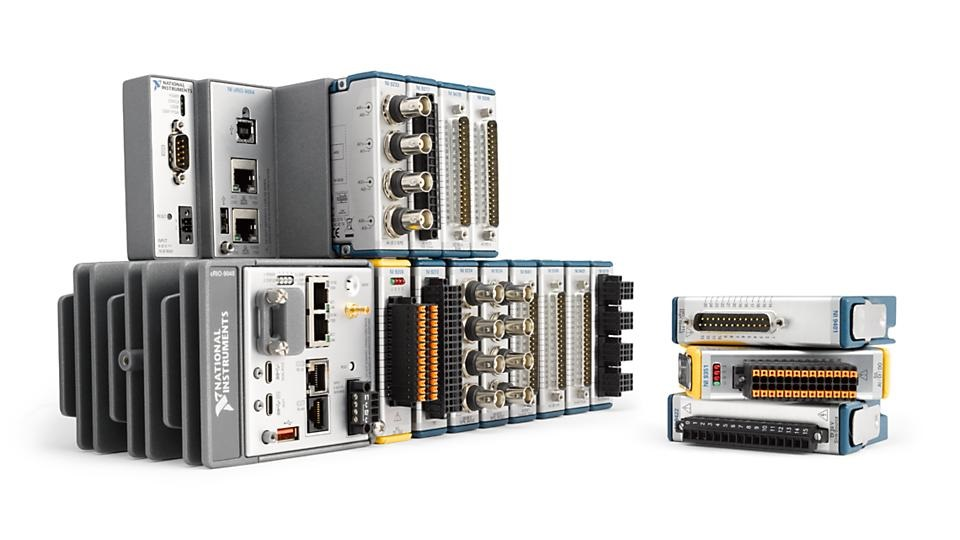
\includegraphics[width=\textwidth]{obrazky-figures/rio.jpg}
    \caption{Jednotka cRIO s~rozšiřujícími moduly \cite{rio}.}
    \label{pic:rio}
  \end{minipage}
  \hfill
  \begin{minipage}[b]{0.45\textwidth}
    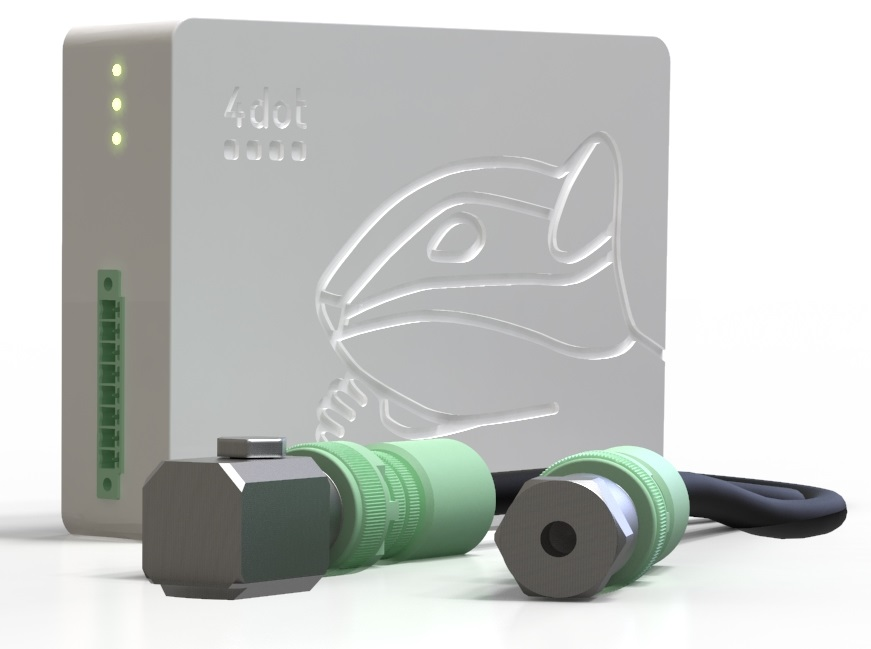
\includegraphics[width=\textwidth]{obrazky-figures/chipmunk.jpg}
    \caption{Jednotka Chipmunk se senzory vibrací \cite{4dotchipmunk}.}
    \label{pic:4dotchip}
  \end{minipage}
\end{figure}


\subsection{Softwarové řešení}
Softwarové řešení pro sběr a zpracování dat má dvě základní části. První částí je softwarové vybavení, kterým jsou vybaveny jednotky. Ty data sbírají, a v~omezené míře i zpracovávají. Druhou částí řešení jsou centralizované serverové aplikace sbírající a zpracovávající data od jednotek. Tyto aplikace se starají také o~přístup k~výsledným informacím a jejich vyhodnocení. 
Existují i lokální řešení, která jsou omezena pouze na jednotku poskytující informace přímo u~monitorovaného stroje (například na monitor). Tyto jednotky dále nekomunikují s~jinými zařízeními. Takovým systémům se však tato podsekce nevěnuje, protože nesplňují cíl Průmyslu 4.0 -- úplné propojení všech částí do jednoho celku.

Software obsažený v~jednotkách je často vytvořen přímo firmou, která vyvinula dané zařízení. Se systémem komunikuje pomocí řady standardizovaných protokolů určených pro průmysl. Příkladem může být jednotka pro monitorování vibrací společnosti ifm\footnote{https://www.ifm.com/gb/en/category/070/070\_010/070\_010\_015\#!/S/BD/DM/1/D/0/F/0/T/24} s~možností výběru komunikačního rozhraní jako je PROFINET IO, Modbus, EtherCAT. Jinou cestou se vydala již zmíněná americká společnost National Instruments, která prodává jednotky bez softwarového vybavení. Programy pro tyto jednotky se vytváří v~programu zvaném LabView\footnote{https://www.ni.com/cs-cz/shop/labview.html} a opět lze volit různá komunikační rozhraní. Více informací ke komunikačním protokolům je obsaženo v~sekci \ref{sec:networkComm}.

\begin{figure}[h]
  \centering
  \scalebox{0.29}{
        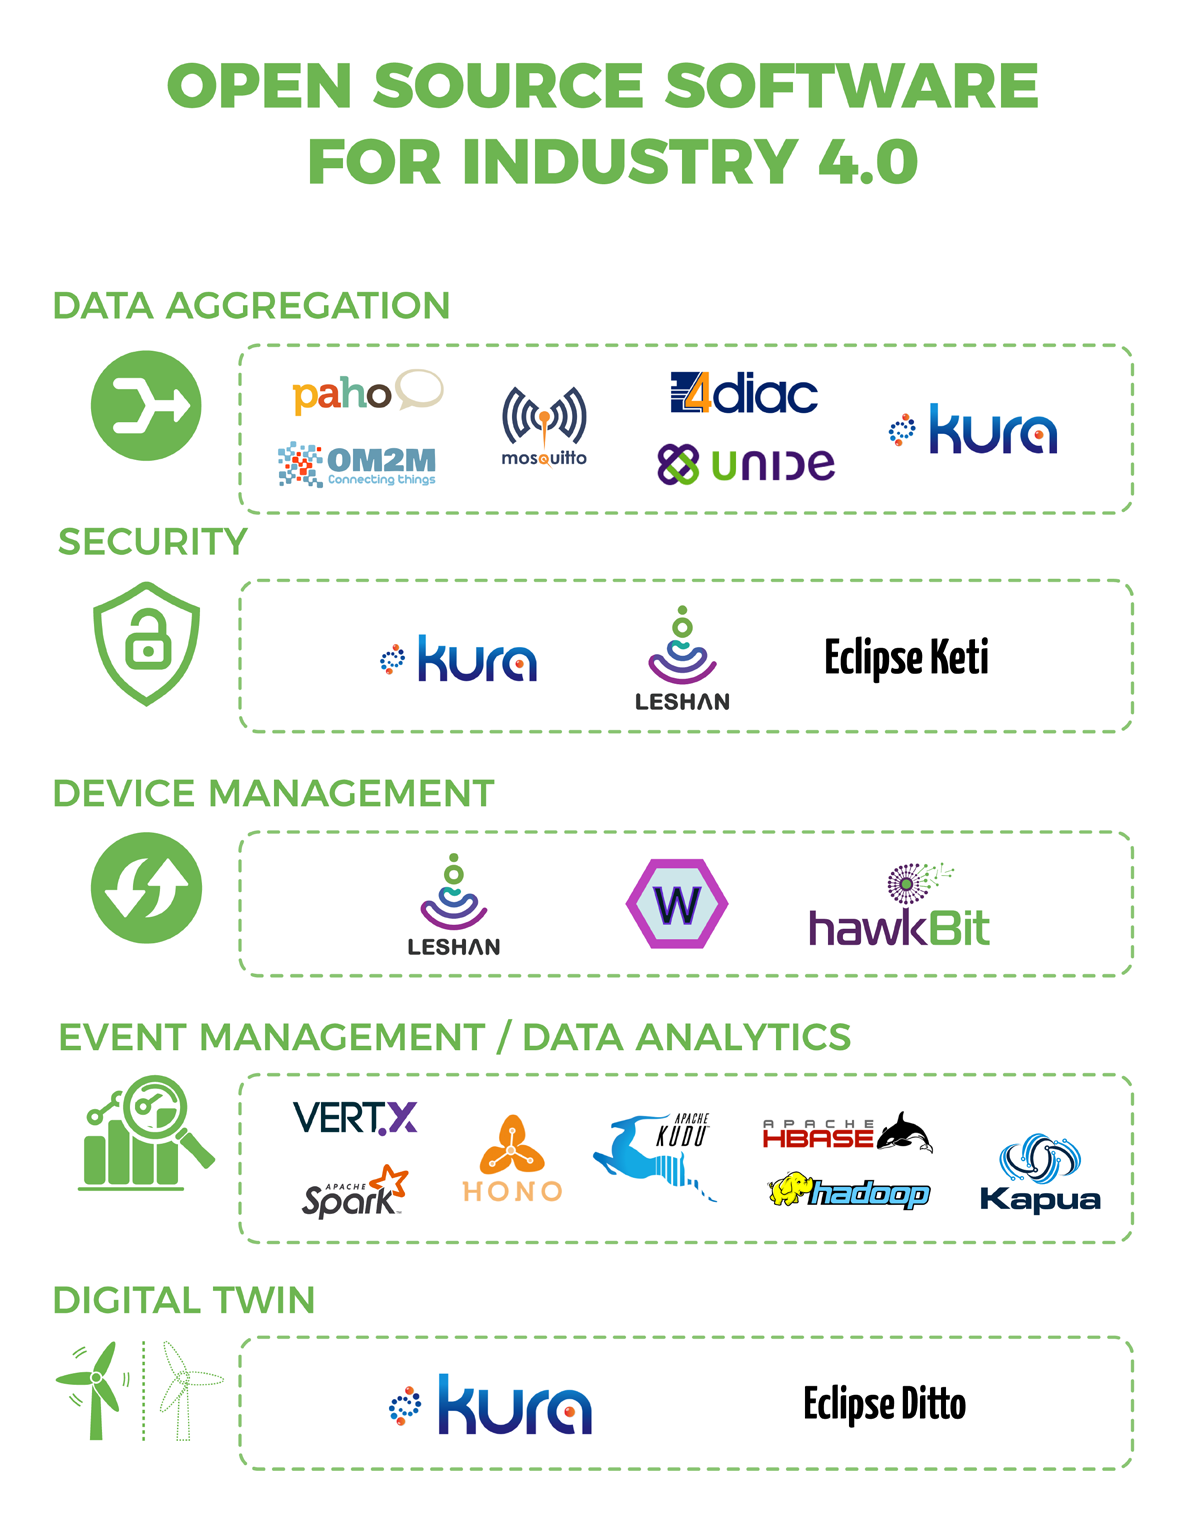
\includegraphics{obrazky-figures/open_source_iot.png}
    }
  \caption{Kategorie komponent systému pro Průmysl 4.0 a jejich zástupci \cite{eclipse}.}\label{pic:eclipseIOT}
\end{figure}

Serverová část systému slouží k~příjmu dat od jednotek, jejich zpracování a uložení. Tyto systémy mohou mít mnoho funkcí a řadu různých komponent. Komponenty se mohou dělit podle funkce do několika kategorií: příjem dat a agregace, zabezpečení, správa zařízení, správa událostí, datové analýzy, datová úložiště a další. Existuje velké množství implementací jednotlivých komponent a to nejen placené, ale i volně dostupné pod open-source licencemi. Příklady zástupců jednotlivých kategorií jsou zobrazeni na obrázku \ref{pic:eclipseIOT}.

Implementaci některých komponent nabízí společnost Eclipse. Příkladem může Eclipse Paho a Eclipse Mosquitto implementující protokol MQTT  (Message Queuing Telemetry Transport). Velká sada softwarových komponent vhodných pro Průmysl 4.0 spadá pod Apache Software Foundation, která obsahuje mimo jiné i nástroje pro distribuované zpracování dat a výpočty či distribuovaná úložiště \cite{eclipse}.

Serverové řešení jako takové tedy není omezeno na jednu určitou implementaci jako u~jednotek, ale je možné vybírat z~různých volně dostupných či placených komponent a postavit systém na míru podle potřeby a využití.

%Například Apache Hadoop je nástroj sloužící pro distribuci zpracovávání velkého množství dat na více výpočetních uzlů s důrazem na snadnou škálovatelnost





%\chapter{Sběr a zpracování velkých dat}\label{kap:bigData}
\chapter{Zpracování velkých dat}\label{kap:bigData}
Získaná data je potřeba zpracovat a vytěžit z~nich co největší množství důležitých informací. Při menším objemu dat se nejedná o~větší problém, ale pokud se bavíme o~velkých datech, u~kterých je potřeba zpracovávat i několik milionů hodnot za vteřinu, nastávají potíže. Programy pro zpracovávání velkých dat jsou obvykle součástí celých systémů pro práci s~velkými daty včetně úložišť, vizualizačních programů a často jsou právě s~úložišti pevně spjaté. Takovým příkladem je Kapacitor, který je součástí platformy Tick, jejíž schéma je vidět na obrázku \ref{pic:tick}. Způsob zpracování také závisí na povaze dat. Nejzákladnějším rozdělením zpracování velkých dat je proudově a blokově orientované.

\section{Proudově orientované zpracování}
Informace o~proudově orientovaném zpracování dat pochází z~\cite{BigDataPlatforms}. Jedná se o~zpracování toku dat v~reálném čase, data jsou tudíž zpracovávána okamžitě při příchodu a ukládají se až po zpracování. V~některých aplikacích data po zpracování ukládána ani nejsou, a to z~důvodu jejich obrovské velikosti. Tento přístup se využívá v~případech, kdy je vyžadována nízká odezva mezi příchodem dat a jejich efektem. Efektem může být výstup v~podobě upozornění pro uživatele. Tato podmínka je kritická pro všechny typy monitorování. Ať už jde o~kontrolu síťového provozu, protipožární ochranu či detekci poruch na průmyslových strojích. Nízká odezva je extrémně důležitá pro rychlé reakce v~případech nenadálých událostí. Tuto podmínku nemůže splnit zpracování po blocích. 

Proudově orientované zpracování musí zajišťovat vysokou dostupnost, aby veškeré události byly ihned zpracovány. Toho se dosahuje pomocí:
\begin{itemize}
    \item distribuce zpracování na několik uzlů a možnosti další škálovatelnosti,
    \item replikace zpracování, při poruše jednoho uzlu lze zachytit událost na jiném uzlu a nedochází ke ztrátě dat,
    \item zpracování ve vnitřní paměti pro dosažení co nejmenší odezvy po příchodu dat a jejich zpracováním, 
    \item paralelního zpracování proudu.
\end{itemize}

Jedním z~příkladů frameworku implementujícího zpracování v~reálném čase je Kapacitor či Apache Spark. Apache Spark poskytuje rozhraní pro psaní programů a jejich distribuci na výpočetních uzlech. Spark zajišťuje toleranci chyb a škálovatelnost stejně jako model MapReduce a může zapisovat do všech databází využívající tento model. Knihovna Spark Streaming poskytuje rozšíření o~možnost zpracovávání dat v~reálném čase s~vysokou propustností. Spark mimo jiné také poskytuje možnost integrace s~nástroji z~Apache hadoop, které jsou původně zaměřené na blokové zpracování dat. 

\section{Blokově orientované zpracování}
Tato metoda zpracovává data po blocích, které již byly shromážděny v~paměti. Nevýhodou tedy je zpoždění získání výsledků analýz z~přijatých dat. Využívá se v~oblastech, kde není potřeba rychlé zpracování hodnot. Například při periodických výpočtech maxim, minim či středních hodnot z~dat uložených v~časových databázích. Jedním z~programů, který poskytuje zpracování po blocích dat čtených z~časové databáze InfluxDB, je Kapacitor. Kapacitor tedy nabízí obě možnosti zpracování dat, je proto vhodný jak pro sledování událostí v~reálném čase, tak pro generování zpráv za delší časové období \cite{batchProcessing}.

\subsection*{MapReduce}
Zdrojem této podsekce je \cite{MapReduce}. Mimo později vyvinutý Apache Spark zmíněný výše je Apache Hadoop primárně zaměřený na zpracovávání dat po blocích. K~tomu využívá framework MapReduce. Jedná se o~programovací model pro zpracování velkého množství dat po blocích pomocí paralelizace a je implementován v~mnoha programovacích jazycích. Celý proces probíhá ve 4 fázích -- rozdělení, mapování, míchání a redukování. Celý postup zpracování jednoho požadavku na výpočet počtu jednotlivých slov ve větě je vidět na obrázku \ref{pic:MapReduce}. Vstupem jednotlivých fází je dvojice klíč-hodnota. Vstup se zpracovává uživatelem definovanou mapovací a redukční funkcí. Jednotlivé fáze provádí:
\begin{itemize}
    \item v~rozdělovací fázi dochází k~rozdělení vstupních dat na formát, který zpracovává mapovací funkce,
    \item mapovací fáze vytvoří výsledek pomocí mapovací funkce, v~našem případě se jedná o~dvojici obsahující slovo a počet výskytů toho slova,
    \item následně při míchání dochází k~setřídění výsledků,
    \item a v~poslední fázi redukce dojde k~agregaci a odeslání výsledku uživateli.
\end{itemize}

\begin{figure}[h]
  \centering
  \scalebox{0.39}{
        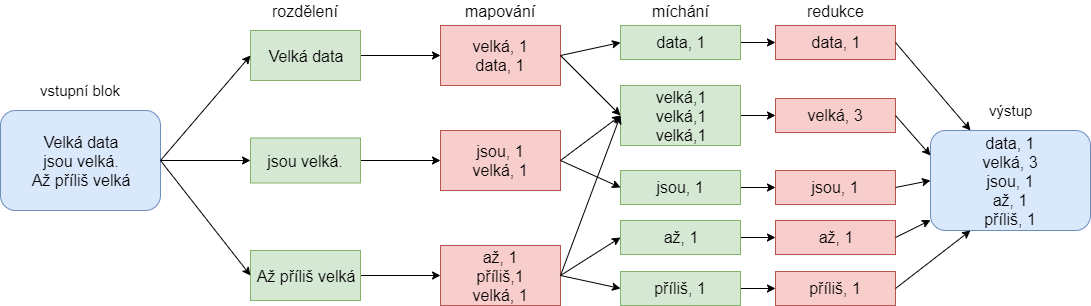
\includegraphics{obrazky-figures/mapReduce.png}
    }
  \caption{Příklad MapReduce modelu pro počítání výskytu jednotlivých slov \cite{MapReduce}.}\label{pic:MapReduce}
\end{figure}

V~praxi je framework MapReduce distribuovaný, tudíž obsahuje více uzlů. Jeden ze serverů přijme požadavek a rozešle úkoly na provedení Map a Reduce funkcí na ostatní uzly. Kvůli zamezení výpadku může provádět i duplicitní výpočet na více uzlech. Po získání výsledků provede dotázaný server zahození duplicitních mezivýsledků a odešle odpověď klientovi.

\section{Zpracování dat ze senzorů vibrací}\label{sec:vibrationAggregation}
%Root mean square, delta treshold, FIR a IIR filtr
Tato sekce čerpá z~\cite{vibrationData}. Pro data z~vibrací je důležitá funkce kvadratického průměru. Kvadratický průměr neboli RMS (Root Mean Square) se vztahuje k~energii vibrací a je důležitým faktorem pro monitorování stavu strojů. Vzorec kvadratického průměru pro blok hodnot je: 
\begin{eqnarray}\label{eq:root_mean_square}
  x_{rms} & = & \sqrt{\frac{\sum_{i=1}^{n} x_i^2}{n}}
\end{eqnarray}
kde $n$ je počet vzorků v~bloku, a $x_n$ je hodnota n-tého vzorku. Dále je pro data z~vibrací důležitá maximální amplituda signálu a Rychlá Furierova Transformace. Rychlá Furierova Transformace se používá pro frekvenční analýzu vibrací která dokáže odhalit abnormální vibrace stroje způsobené poškozením určité součástky.

\section{Komprese dat}\label{sec:compression}
Velká data mohou nabývat velikosti petabajtů nebo i více a je neefektivní je udržovat v~nekomprimované podobě. Ať už jde o~omezení síťové komunikace, či udržování dat na úložišti, je vhodné do určité míry omezit jejich velikost. Zároveň je nutné myslet na budoucí využití komprimovaných dat. Pokud mají být data rychle k~dispozici pro provádění analýz nebo vizualizaci, musí být dekomprimace dat rychlá. Tato sekce se zaměřuje na popis metod využitelných pro body obsahující kombinaci celočíselné časové značky a naměřené desetinné hodnoty. Komprese tohoto formátu je potřebná při čtení a zpracování dat ze senzorů při monitorování strojů, na což je tato práce zaměřená.

\subsection{Delta encoding}\label{sec:delta}
Komprese pomocí metody delta encoding je vhodná pro pravidelně či málo se měnící hodnoty celých čísel, jako je unixová časová značka. Metoda je založená na výpočtu rozdílu sousedních hodnot, vzorec pro výpočet je následující \cite{smith2003digital}:
\begin{eqnarray}\label{eq:delta}
  \Delta_t & = & t_n-t_{n-1}
\end{eqnarray}
Touto metodou může dojít ke snížení rozsahu hodnoty nutné k~uložení čísla. V~případě unixové 32bitové časové značky, která je zaznamenávána při pravidelném měření, může dojít k~citelné kompresi dat. Příklad je možné vidět v~tabulce \ref{tab:delta}. První sloupec tabulky obsahuje nekomprimované časové značky o~velikosti 32 bitů. V~druhém sloupci se nachází $\Delta t$ těchto hodnot. První bod se pouze přesune z~důvodu zachování počátečního bodu a nedojde tedy k~jeho kompresi. K~uložení rozdílů, které v~tomto případě nabývají pouze kladných hodnot, postačí 6 bitů poskytujících rozsah $0\textup{--}127$. Čím výraznější změna mezi hodnotami nastává, tím horších výsledků je dosaženo. Tato metoda tedy nemá smysl pro kompresi například řetězce ASCII znaků. Jak lze vidět na sloupci $\Delta ASCII$, výsledky nabývají i záporných hodnot. K~zakódování jednoho znaku bychom potřebovali 8 bitů. Jelikož je ASCII znak reprezentován 8bitovou hodnotou, nebylo by dosaženo žádného zlepšení \cite{smith2003digital}.

Časová databáze Gorilla (viz \ref{sec:gorilla}) využívá pro kompresi časových značek pozměněnou verzi této metody založenou na podmínce, že měření se opakuje v~pravidelných intervalech. Vzorec \ref{eq:deltadelta} tedy odečítá deltu předchozích hodnot od delty aktuálních hodnot. Hodnoty jsou ukládané po dvouhodinových blocích. Hlavička obsahuje časovou značku zarovnanou na začátek daného dvouhodinového bloku a první delta využívá původní vzorec \ref{eq:delta}, kde $t_{n-1}$ je časová značka z~hlavičky. Hodnoty jsou následně ukládány s~proměnlivou délkou\cite{gorilla}. 
\begin{eqnarray}\label{eq:deltadelta}
  D & = & (t_n-t_{n-1})-(t_{n-1}-t_{n-2})
\end{eqnarray}
Možnost využití této úpravy je viditelná i na vzorových datech v~tabulce \ref{tab:delta}, kde měření probíhá zhruba jednou za minutu. Jak je vidět ve sloupci $\Delta\Delta t$ (počáteční hodnota zarovnaná na začátek dvouhodinového intervalu činí 1577664000), oproti předchozí verzi metody došlo ke kompresi první hodnoty z~32 na 5 bitů a zbylé hodnoty je možné uložit na 4 bitech.

\begin{table}[h]
    \begin{center}
        \begin{tabular}{|c|c|c||c|c|c|}
        \hline
             časová značka & $\Delta t$ & $\Delta\Delta t$ & znak & ASCII hodnota & $\Delta ASCII$ \\ \hline
             1577664060 & 1577664060 & 60 & B & 66 & 66 \\
             1577664120 & 60 & 0 & i & 105 & 39 \\
             1577664178 & 58 & -2 & g & 103 & -2 \\
             1577664239 & 61 & 3 & D & 68 & -35 \\
             1577664302 & 63 & 2 & a & 97 & 29 \\
             1577664361 & 59 & -4 & t & 116 & 19 \\
             1577664425 & 64 & 5 & a & 97 & -19 \\ \hline
        \end{tabular}
        \caption{Příklad výpočtu komprimovaných hodnot Delta encoding pro pravidelné časové značky a řetězec znaků.} \label{tab:delta}
    \end{center}
\end{table}
\subsection{XOR encoding}\label{sec:xor}
Teoretické informace této podsekce pochází z~\cite{gorilla}. Metodu využívá časová databáze Gorilla (viz \ref{sec:gorilla}) pro kompresi desetinných čísel s~dvojitou přesností. XOR encoding funguje na podobném principu delta komprese - ukládá rozdíl sousedních hodnot. Základem metody je operace $\oplus$ (XOR) mezi dvěma po sobě jdoucími čísly. Hodnoty jsou ukládány podle následujících pravidel:

\begin{enumerate}
    \item první hodnota je uložena bez komprese,
    \item pokud je výsledek operace $\oplus$ 0 (hodnoty jsou totožné), uloží se pouze jeden nulový bit,
    \item pokud je výsledek operace $\oplus$ nenulový (hodnoty se liší) a zároveň počet nulových bitů na začátku a konci výsledku \textbf{je} stejný nebo vyšší než u~předchozího výsledku, jako první se uloží kontrolní bity $10$ následované nenulovou částí výsledku operace,
    \item pokud je výsledek operace $\oplus$ nenulový (hodnoty se liší) a zároveň počet nulových bitů na začátku a konci výsledku \textbf{není} stejný nebo vyšší než u~předchozího výsledku, jako první se uloží kontrolní bity $11$, následuje 5 bitů obsahující počet počátečních nul, 6 bitů obsahující délku nenulových bitů a samotné nenulové bity výsledku.
\end{enumerate}

Příklad reprezentace všech tří možností uložení v~paměti je možné vidět v~tabulce \ref{tab:xor}. První hodnota v~paměti je opsána podle pravidla číslo jedna. U~druhé hodnoty nedošlo ke změně, a proto je uložen pouze jeden bit prefixu (prefixy jsou označeny červeně) obsahující nulu podle druhého pravidla. U~třetí hodnoty došlo ke změně, a jelikož je počet nul před a po nenulových bitech nižší (předchozí hodnota má všechny bity nulové), je použito čtvrté pravidlo. První dva bity určují prefix, následujících 5 bitů vyznačených modře označuje počet nulových bitů před hodnotou, 6 bitů označených zeleně obsahuje délku výsledku a poslední je samotný výsledek operace. Čtvrté číslo je uloženo v~paměti pomocí třetího pravidla, protože počet nul před výsledkem je totožný jako u~předchozího a počet nul za výsledkem je o~jednu vyšší. První dva bity opět označují prefix a zbytek obsahuje výsledek.

\begin{table}[h]
 \footnotesize
 \begin{center}
    \begin{tabular}{|c|c|c|c|c|}
        \hline
         dec & hex & $\oplus$ s~předchozí & uloženo v~paměti & velikost [b] \\ \hline
         $19.0625$ & 0x4033100000000000 & - & 0x4033100000000000 & 64 \\
         $19.0625$ & 0x4033100000000000 & 0x0 & $0b$\textcolor{red}{0} & 1 \\
         $41.25$ & 0x4044A00000000000 & 0x0077B00000000000 & 0b\textcolor{red}{11}\textcolor{blue}{01001}\textcolor{green}{001010}11101111011 & 24 \\
         $25.5$ & 0x4039800000000000 & 0x007D200000000000 & 0b\textcolor{red}{10}11111010010 & $13$ \\ \hline
        \end{tabular}
    \caption{Příklad výpočtu komprimovaných hodnot pro XOR encoding.} \label{tab:xor}
    \end{center}
\end{table}

Hlavní výhodou metody je nutnost pouze jednoho bitu k~uložení nezměněné hodnoty a při menších změnách dosahuje několikanásobné komprese. Metoda je tedy vhodná například pro data pořízená z~měření teploty, u~kterých nedochází k~velkým výkyvům. 

\section{Síťová komunikace a zabezpečení} \label{sec:networkComm}
 Mnoho zařízení pro monitorování vzniklých před nebo v~počátcích čtvrté průmyslové revoluce disponuje proprietárními komunikačními protokoly. Tyto protokoly jsou neveřejné a výrazně omezují větší změny v~systému, jako je nákup zařízení od jiných výrobců či napojení na novější systémy. Postupem času začaly vznikat otevřené standardy jako je MODBUS TCP či EtherCAT pro lokální komunikaci. Upuštění od proprietárních komunikačních protokolů tedy značně usnadňuje vytvoření a propojení systémů IIoT (Industrial internet of things) od různých výrobců do jednoho celku.

MODBUS je bitově orientovaný asynchronní komunikační protokol využívající TCP, určený pro výměnu informací mezi vestavěnými systémy a průmyslovými aplikacemi. Protokol využívá takzvaný \textit{pooling} neboli aktivní dotazování metodou dotaz-odpověď. Pomocí dotazu si lze vyžádat data či provést příkaz. Odpověď obsahuje potvrzení provedení vyžadovaného příkazu či vyžádaná data. Další protokol, který se využívá, je MQTT. Jedná se opět o~TCP protokol, je oproti protokolu MODBUS synchronní a využívá model \textit{publisher–subscriber} (vydavatel-odběratel). O~výměnu zpráv se stará jeden centrální bod zvaný MQTT broker. Ten zprávy přijímá od vydavatelů, třídí do takzvaných témat a rozesílá všem odběratelům, kteří jsou k~danému tématu přihlášeni \cite{iotComm}. 

Standardizované protokoly nejsou vhodné pro každé využití. Jsou určeny spíše pro informování o~změně stavu v~lokální síti a ne pro zasílání velkého množství dat pro zpracování přes internet. Protokoly vyžadují výměnu mnoha zpráv, takzvaných \textit{handshake} zpráv, před zasláním samotné zprávy s~informacemi, a nejsou zabezpečeny. Pro zasílání většího množství zpráv přes internet je vhodnější využít vlastních zjednodušených a zabezpečených UDP či TCP protokolů. Komunikaci přes TCP lze zabezpečit pomocí SSL (Secure Sockets Layer) certifikátu, který vytváří šifrované spojení.
%https://sites.google.com/site/amitsciscozone/home/security/ssl-connection-setup
UDP pakety lze zabezpečit například pomocí DTLS (Datagram Transport Layer
Security) či jednoduchou bitovou operací XOR.
%https://tools.ietf.org/html/rfc6347


%https://www.researchgate.net/publication/331588782_Communication_Protocols_of_an_Industrial_Internet_of_Things_Environment_A_Comparative_Study

\section{Vizualizace a vyhodnocení velkých dat ze senzorů}
Vizualizace dat ze senzorů při využití existujících řešení často úzce souvisí se zvoleným úložištěm. Téměř každé úložiště velkých dat je možné propojit s~nějakou vizualizační aplikací. Jednou z~nejrozšířenějších vizualizačních aplikací je Grafana a slouží i k~analýze dat. Grafana je volně dostupná a jedná se o~aplikaci s~webovým rozhraním, schopnou pracovat s~daty z~několika různých databází. Grafana podporuje mimo jiné i časové databáze, jako je InfluxDB či Graphite \cite{grafana}. Vzhled aplikace je na obrázku \ref{pic:grafana}. 

Časová databáze InfluxDB, která je součástí ekosystému TICK, nabízí i vlastní grafické rozhraní Chronograf včetně analytického nástroje Kapacitor. Chronograf zobrazený na obrázku \ref{pic:installsdf} nabízí podobné uživatelské rozhraní jako Grafana. V~těchto rozhraních je možné využívat veškeré databázové dotazy, včetně importování či exportování hodnot. Lze vytvářet nástěnky s~uloženými dotazy, sledovat hodnoty přicházející do databáze v~reálném čase či sledovat vytížení samotné databáze. Analyzační nástroj Kapacitor oproti tomu slouží k~detekci nastavených událostí, jako je například překročení limitu \cite{Influx}. Podobné nástroje jsou dostupné pro téměř každé úložiště velkých dat v~rámci jejich ekosystémů.



\begin{figure}[h]
  \centering
  \scalebox{0.70}{
        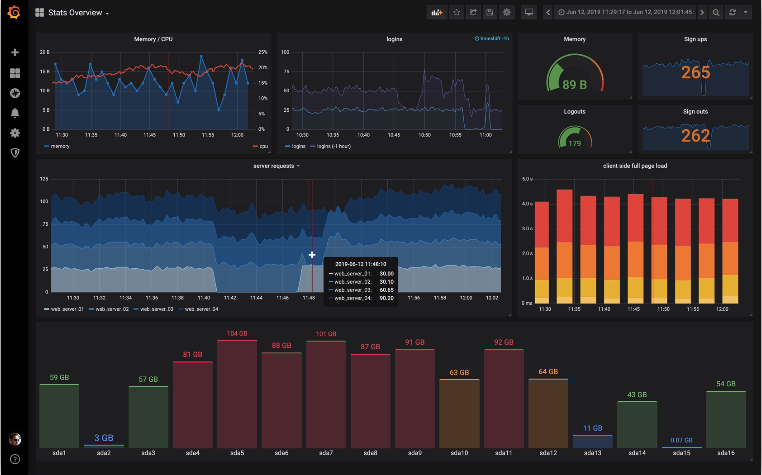
\includegraphics{obrazky-figures/grafana.png}
    }
  \caption{Webové rozhraní aplikace Grafana \cite{grafana}.}\label{pic:grafana}
\end{figure}

%v článku big data processing jsou tři postupy, analytický, matematický, data mining
%Kromě základního přístupu k datům v podobě konzolového rozhraní které nabízí většina databází i

%api rest, ale zmínit přímo napojení na data pomocí SQL-on-Hadoop
%příklad jak to funguje? vkládání a tak?


\chapter{Úložiště velkých dat}\label{kap:storage}
S~přibývajícím množstvím moderních technologií a odvětví (například IoT -- Internet of Things) vznikají nové problémy s~množstvím dat, které generují. Ať už jde o~záznamy o~uživatelích sociálních sítí, souřadnice polohy osob či vozidel sbíraných chytrými telefony, historii nákupů na internetovém obchodě nebo měření ze senzorů, je potřeba tyto informace  uchovávat a zároveň musí být rychle a snadno dostupné pro zpracování. Jelikož se může jednat o~obrovské množství dat, nároky na tyto systémy jsou velmi vysoké. Pro představu o~jaké množství dat může jít si vezměme například službu Timeline od společnosti Google. Při povolení této služby chytrý mobilní telefon snímá polohu přístroje a vlastník připojeného účtu má zpětně přehled o~svém pohybu a činnostech. Během dne může být takto vygenerováno od pár desítek po několik tisíc záznamů, které je potřeba uložit a v~případě potřeby zpřístupnit. Samo o~sobě se nejedná o~velké množství dat, ale když vezmeme v~úvahu množství lidí využívající chytrý telefon, mluvíme zde o~sta milionech záznamů denně. 

K~ukládání takového objemu dat se využívají mimo jiné distribuované souborové systémy, cloudové nástroje či specializované databázové systémy. Tato kapitola je věnována různým typům úložišť pro tato data a je zaměřena na řešení určené pro ukládání hodnot získaných během měření různých senzorů. U~tohoto typu dat je nejdůležitějším údajem každého záznamu kombinace času měření a naměřené hodnoty. Kapitola má tedy za cíl seznámit čtenáře s~technologiemi, které se často využívají pro ukládání velkých dat a s~vysvětlením jejich principů.

\section{NoSQL}
Jedná se o~nerelační datový model podporující distribuovanou architekturu a umožňující zpracování velkého množství dat - až petabajty dat za den. Oproti relačnímu modelu obětuje přílišnou komplexnost způsobující striktní zajištění pravidel ACID (Atomicity, Consistency, Isolation, Durability) tzn. atomičnost transakcí, konzistenci dat, neovlivnění souběžných transakcí a ochrana proti ztrátě transakcí. Tato ztráta komplexnosti sice umožňuje inkonzistenci a nepřesnost, to ale kompenzuje vysokou propustností a škálovatelností. Tento model je proto vhodný pro data, u~kterých nejsou drobné nepřesnosti problematické a je potřeba jich zpracovávat obrovské množství, jako například u~sledování dat ze senzorů či monitorování sítě a podobně. Tento model je proto naprosto nevhodný k~uchování dat vyžadující konzistenci (například bankovní transakce), kde i ztráta jednoho záznamu může znamenat katastrofu. Ztráta záznamu ale není velkým problémem třeba u~monitorování síťového vytížení, kde se stejně agreguje obrovské množství hodnot a nedojde proto k~velkému ovlivnění výsledku. Možnost nezajistit konzistenci proto dovoluje právě povaha dat, pro která jsou úložiště využívající tento model určena \cite{NoSQL}.

\section{Hadoop Distributed File System} \label{HDFS}
Hadoop Distributed File System (dále jen HDFS) je součástí volně dostupného projektu Apache Hadoop. Jedná se o~distribuovaný souborový systém poskytující vysokou propustnost dat a toleranci poruch. V~této sekci a jejích podsekcích byly informace čerpány z~dokumentace projektu HDFS\cite{HDFSDoku}.

\subsection{Architektura HDFS}
HDFS využívá architekturu master/slave a je distribuovaný, tudíž využívá více datových uzlů. Samotné blokové schéma systému je zobrazena na obrázku \ref{pic:hdfs_architecture}. Datové uzly se starají o~samotné úložiště. Většinou je umístěn právě jeden datový uzel na fyzickém serveru. Umístění více instancí uzlu na jeden fyzický server nepřidává žádné výhody. HDFS umožňuje uživateli ukládat data do souborů, které jsou následně rozděleny na bloky a ty jsou distribuovány mezi několik datových uzlů. Datové uzly se také starají o~veškeré operace s~bloky - vytváření, mazání, replikace, čtení a zápis.

\begin{figure}[h]
  \centering
  \scalebox{0.50}{
        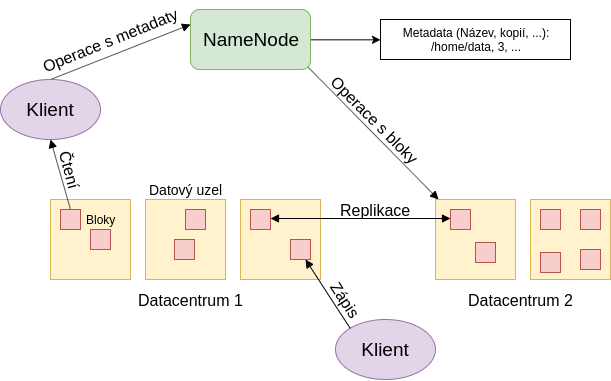
\includegraphics{obrazky-figures/HDFSarchitecture.png}
    }
  \caption{Schéma architektury HDFS \cite{HDFSDoku}.}\label{pic:hdfs_architecture}
\end{figure}

Všechny bloky souboru mají stejnou velikost - vyjma posledního. Jednotlivé bloky jsou replikovány napříč uzly a tím se dosahuje tolerance poruch uzlů. Velikost bloků a počty jejich kopií (replikační faktor) jsou nastavitelné pro každý soubor zvlášť a tyto hodnoty jsou udržované v~metadatech. Soubor v~HDFS lze zapsat pouze jednou a jedním uživatelem. 

Datové uzly spravuje \textit{NameNode}. Jedná se o hlavní server, který se stará o~hierarchii souborového systému, metadata a upravuje přístup klientům. Jakoukoliv změnu umístění či vlastností (například replikační faktor, název, id) zaznamenává do logu a mění v~metadatech. \textit{NameNode} se stará o~veškerá rozhodnutí týkající se replikace bloků. Od každého datového uzlu periodicky dostává upozornění indikující správnou funkčnost (takzvaný \textit{Heartbeat}) a seznam jednotlivých uložených bloků. 


\subsection{HBase} \label{Hbase}
HBase je taktéž součást Apache Hadoop a jedná se o~sloupcově orientovaný nerelační databázový systém operující nad HDFS (viz \ref{HDFS}). HBase je nástroj vhodný pro zpracovávání dat v~reálném čase, náhodný přístup k~velkému množství dat a je lineárně škálovatelný. Nepodporuje strukturované dotazy jako SQL. Systém lze lineárně škálovat. Každá tabulka musí obsahovat primární klíč a k~uloženým datům lze přistupovat pouze přes tento primární klíč \cite{HBase}.

\section{Google BigTable}\label{sec:bigtable}
Jedná se o~distribuovaný systém využívaný pro ukládání dat a je navržen tak, aby byl schopný pracovat s~ohromným množstvím dat na velkém počtu serverů. V~této sekci čerpám informace z~\cite{BigTable}.

BigTable je multidimenzionální tříděná mapa. Základní jednotkou je netypovaný řetězec znaků, který je interně uložený v~blocích ve tříděných tabulkách řetězců znaků zvaných SSTable. Tyto bloky jsou dostatečně malé na to, aby je bylo možné nahrát do operační paměti (typicky 64 kB). Na konci každé tabulky je uložen index, který je nahrán do paměti při otevření tabulky. BigTable indexuje podle řetězce znaků, přesněji podle řádku, sloupce a verze (většinou se jedná o~časovou značku). Záznamy mají lexikografické uspořádání. Tabulky jsou ukládány po blocích zvaných \textit{tablet} podle rozsahu a pokud tento blok překročí určitou velikost, je rozdělen na dva tablety (bloky jsou typicky 100-200 MB velké). Schéma tabletu je možné vidět na obrázku číslo \ref{pic:tablet}. Každý záznam obsahuje verzi, která je záznamům přidělována automaticky jako časová značka aktuálního času při zápisu, tím se předchází možným kolizím hodnot. Verzi lze přidělovat i z~klientské aplikace, která BigTable využívá, ale potom je na klientské aplikaci, aby zajistila unikátnost záznamů. Verze záznamu je využívána pro mazání starých a neaktuálních hodnot. Klient může specifikovat kolik záznamů nebo jaký časový úsek do minulosti má být uchováván.

Samotný systém obsahuje dva typy serverů - master a tablet server. Master server je puštěn pouze v~jedné instanci a stará se o~rozdělení tabletů tablet serverům, detekci expirace tablet serverů, vyvažování zatížení, zálohy a změny schémat systému. Tablet servery se starají o~tablety, zápis, čtení a rozdělení tabletů při překonání určité velikosti. Klientské aplikace komunikují přímo s~tablet servery. Ke správě záloh se využívá služba zvaná \textit{Chubby}. Pro zjištění polohy uložených dat slouží tříúrovňový B-strom, obsahující metadata o~tabletech. 

\begin{figure}[h]
  \centering
  \scalebox{0.43}{
        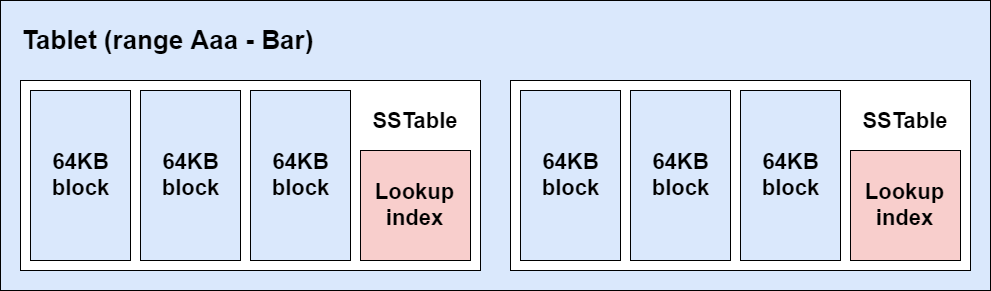
\includegraphics{obrazky-figures/bigtable_tablet.png}
    }
  \caption{Schéma tabletu \cite{BigTableTablet}.}\label{pic:tablet}
\end{figure}

\section{Time-series databáze}
Časová databáze (lépe známé pod anglickým názvem \textit{time-series database}) je speciálním typem databáze určené a optimalizované pro zaznamenávání měření obsahující časovou značku. Tyto databáze se využívají ve finančním sektoru (historie stavu akcií pro predikce jejich budoucího vývoje), telekomunikacích (informace o~stavu a využití sítí), nebo při monitoringu datových center (monitorování teploty, využití procesorů, poruch) či průmyslových strojů.

Jak už tedy název napovídá, pracují s~časovou značkou, která se vyskytuje u~každého záznamu, a je vždy primárním klíčem nebo alespoň jeho součástí. Časová databáze typicky obsahuje datové body, které představují měření v~daném čase.  Oproti relačním databázím se téměř nepočítá s~využitím funkcí pro aktualizaci (UPDATE) či mazání (DELETE) hodnot a dotazy (SELECT) jsou velmi specifické. Složité složené dotazy plné podmínek nejsou časté pro data tohoto typu a nejčastějším typem dotazů je získání určitého časového okna měřených dat, a to co nejefektivněji. Právě na tyto dotazy jsou časové databáze optimalizovány\cite{time-series-paper}. 

Časové databáze jsou obvykle postaveny nad distribuovanými souborovými systémy, jako jsou HDFS či Bigtable popsané dříve v~této kapitole, a s~jejich pomocí dosahují vysoké rychlosti čtení a zápisu hodnot a škálovatelnosti systému.

Kromě času obsahují časové databáze jako OpenTSDB nebo InfluxDB dva další typy hodnot - značky (\textit{tag}) a datová políčka (\textit{field}). Databáze následně zajišťuje unikátnost záznamu pomocí primárního klíče složeného z~kombinace času, značek a měřené hodnoty. Záznamy jsou následně ukládány v~balících podle značek a v~těchto balících jsou seřazeny podle času. Tento přístup zrychluje možnost agregace uložených hodnot \cite{time-series-book}.

\subsection{Řádkově/sloupcově orientované ukládání}
Databáze využívají k~ukládání dat dva způsoby - jsou sloupcově nebo řádkově orientované. Řádkově orientovaná metoda je používaná relačními databázemi. Ukládá a získává data po řádcích. Tento způsob uložení není efektivní pro agregaci a analýzu většího množství hodnot a dosahuje horší úrovně komprese dat než ukládání po sloupcích. Čtení a zápis je ale snazší. Sloupcově orientované databáze oproti tomu ukládají a získávají data po sloupcích. Příkladem je HBase, která je základem některých časových databází. Touto metodou lze dosáhnout rychlé agregace velkého množstvím hodnot a umožňuje vysokou úroveň komprese díky podobnosti hodnot, které jsou za sebou uložené. Přestože sloupcově orientované databáze dominují úložištím velkých dat, lze nalézt i databáze které kombinují oba způsoby, jako je TimescaleDB \cite{rowColumn}.

\subsection{Zástupci}
S~rostoucí potřebou zpracování a uložení dat z~měření se v~posledních letech rozšířil počet různých časových databází. Nejedná se již jen o~obecné implementace jak tomu bylo dříve, ale i o~databáze určené ke specifickým účelům, na míru vyvinutým potřebám firem, jako je Facebook či Google. Nejznámější a nejpoužívanější time-series databáze jsou následující:

\subsubsection*{OpenTSDB}
Jedná se o~škálovatelnou volně dostupnou časovou databázi pracující nad HBase (popsanou v~\ref{Hbase}) či Google Bigtable (popsaný v~sekci \ref{sec:bigtable}). OpenTSDB nabízí rozhraní pro zápis a čtení a stará se o~veškeré operace související se správou HBase. Data lze získat v~grafické formě či ve formě souboru ve formátu json.

Jak je vidět na obrázku \ref{pic:OpenTSDB}, OpenTSDB je vlastně několik samostatných TSD instancí, které zastřešují přístup k~úložišti a starají se o~veškerou komunikaci. Uživatel tedy přistupuje k~datům pouze s~pomocí poskytnutého rozhraní. Databáze je optimalizovaná pro rychlou agregaci hodnot. Čas je uložen ve formě unixové časové značky a hodnoty jsou 64bitová celá či desetinná čísla. Přístup k~datům je možný pomocí vestavěného grafického rozhraní či přes HTTP rozhraní \cite{TSDBdoku}.

\begin{figure}[!tbp]
  \centering
  \begin{minipage}[b]{0.45\textwidth}
    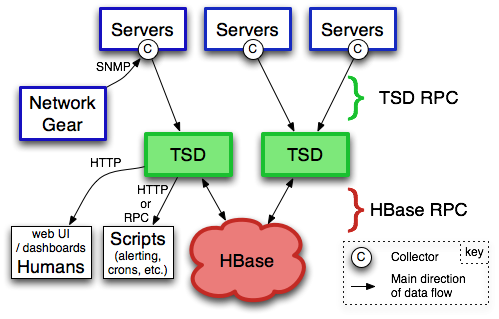
\includegraphics[width=\textwidth]{obrazky-figures/tsdb-architecture.png}
    \caption{Architektura OpenTSDB \cite{TSDBdoku}.}
    \label{pic:OpenTSDB}
  \end{minipage}
  \hfill
  \begin{minipage}[b]{0.45\textwidth}
    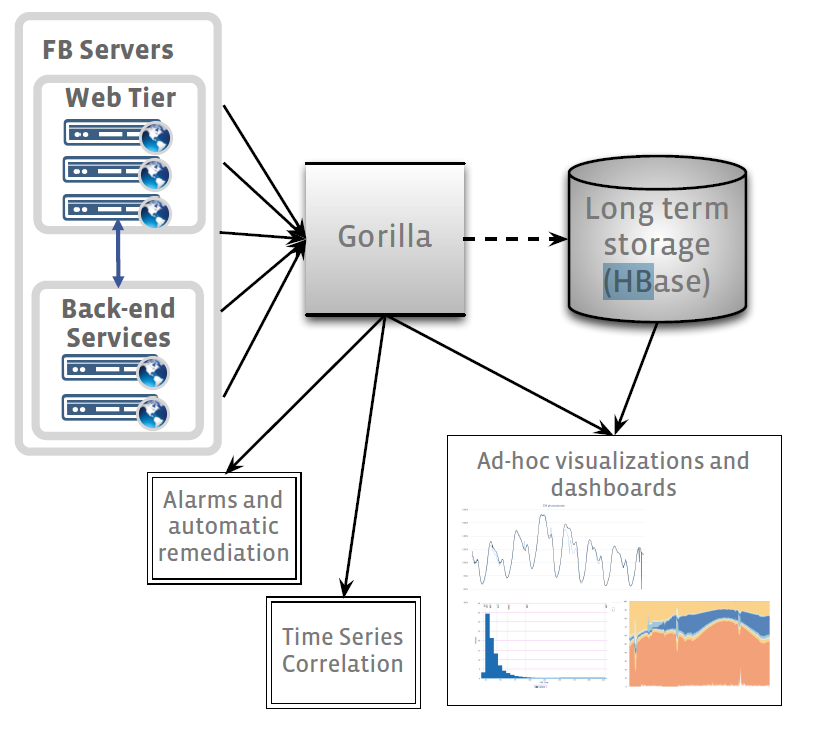
\includegraphics[width=\textwidth]{obrazky-figures/gorilla.PNG}
    \caption{Schéma využití databáze Gorilla \cite{gorilla}.}
    \label{pic:gorilla}
  \end{minipage}
\end{figure}

\subsubsection*{InfluxDB}
Informace o~InfluxDB byly čerpány z~\cite{Influx}. Databáze InfluxDB byla vytvořena již od základu jako časová a je k~dispozici volně dostupná i v~komerční verzi. Jedná se o~NoSQL databázi implementovanou v~jazyce Go. Komerční verze nabízí dodatečnou funkcionalitu nutnou pro nasazení ve větším měřítku - například možnost využití instancí na více serverech či pokročilé monitorování. Jedná se o~nejpopulárnější časovou databázi. InfluxDB se skládá z databází, které obsahují jednotlivé hodnoty uspořádané podle měření (\textit{Measurement}). Měření se dá přirovnat k~tabulkám. Záznam obsahuje název měření, set tagů podle kterých se indexuje, set hodnot podle kterých se neindexuje a časovou značku v~přesnosti na nanosekundy. Počet tagů není omezený na rozdíl od OpenTSDB. InfluxDB poskytuje jazyk pro dotazy podobný SQL dotazům. Pro každé měření lze nastavit jak dlouho a v~kolika kopiích mají být hodnoty uchovány. InfluxDB využívá svůj vlastní úložný engine zvaný TSMT (Time Structured Merge Tree). Databáze ukládá data po blocích zvaných \textit{shard}, které jsou organizovány podle nastavení životnosti dat do časových úseků. Základní časový úsek pro životnost dat kratší než dva dny je jedna hodina, a pro životnost delší než 6 měsíců je časový úsek jednoho bloku 7 dní.

\begin{figure}%[h]
  \centering
  \scalebox{0.43}{
        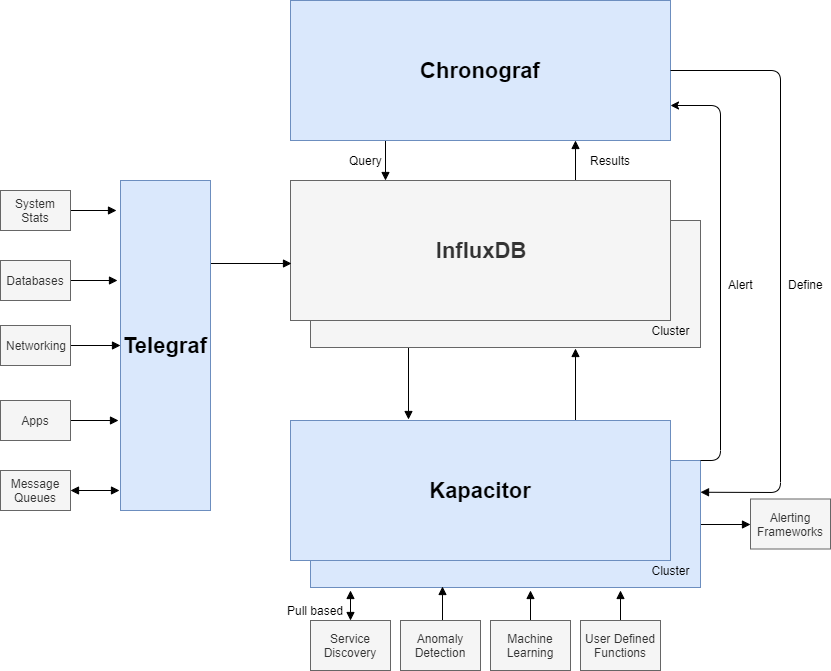
\includegraphics{obrazky-figures/influx.png}
    }
  \caption{Schéma platformy Tick \cite{Influx}.}\label{pic:tick}
\end{figure}

K~datům lze přistupovat přes HTTP a UDP komunikační rozhraní, přes konzoli podobně jako u~MySQL či přes webovou aplikaci Chronograf. InfluxDB a Chronograf jsou součástí platformy TICK. Součástí této platformy je i modul Telegraf, který slouží k~monitorování serverů, na kterých je spuštěn InfluxDB, a engine pro zpracovávání dat v~reálném čase Kapacitor. 
Na obrázku číslo \ref{pic:tick} je znázorněno schéma platformy TICK s~databází InfluxDB ve svém jádru.

\subsubsection*{Gorilla} \label{sec:gorilla}
Technické informace této části pochází z~\cite{gorilla}. Gorilla je \textit{in-memory} databáze (data jsou uložena v operační paměti) vytvořená firmou Facebook, která slouží pro monitorování dat zapisovaných do HBase databáze. Vizualizované využití této databáze je možné vidět na obrázku \ref{pic:gorilla}. Bod uložený v~databázi obsahuje klíč ve formě posloupnosti znaků, 64bitové časové značky a desetinného čísla obsahujícího hodnotu. Jelikož se jedná o~\textit{in-memory} databázi, která funguje jako mezipaměť pro dlouhodobější uchování dat na discích, jsou hodnoty udržovány po omezenou dobu. Množství bodů je ale natolik velké, že požadavky na paměť by byly v~řádech desítek terabajtů, proto databáze využívá kompresních algoritmů popsaných v~\ref{sec:delta} a \ref{sec:xor}. Tento algoritmus umožňuje průměrnou kompresi 16 bajtů na 1,37 bajtu. Gorilla se také od ostatních časových databází odlišuje svou úzkou specializací na monitorování systémů v~reálném čase. Databáze má za cíl co nejrychleji odhalovat chyby v~interních systémech. Databáze musí být schopná bez výpadku přijímat a zapisovat velké množství bodů i za cenu dočasné nedostupnosti pro čtení nebo ztráty starších bodů. Proto není kladen důraz na jednotlivé body, ale na agregované analýzy. Gorilla je distribuovaná mezi několik regionů bez zajištění konzistence a dotazy jsou směrovány na nejbližší datová centra. To umožňuje tolerovat výpadek celého regionu.

Hodnoty jsou uloženy ve formě \textit{TSMap}. Ta je složena z~vektorů sdílených ukazatelů na časové série a mapy obsahující dvojice název série a ukazatel na její umístění v~paměti. Při smazání série nejsou data smazána, ale paměť je pouze označena pro znovupoužití. Výlučný přístup k~datům zajišťuje zámek na \textit{TSmap} a 1-bajtový zámek s~aktivním čekáním na každé časové sérii.

\subsubsection*{TimescaleDB}
Zdrojem informací o~architektuře TimescaleDB je \cite{TimescaleDoku}. Oproti výše zmíněným databázím je TimescaleDB založená na relačním databázovém modelu využívající PostgreSQL. TimescaleDB je zaměřená na lepší paralelní zpracování a škálování nejen na více uzlů, ale i na jednom samotném uzlu. Je ale nutno zmínit, že v~době psaní této práce bylo škálování na více uzlů stále ve fázi vývoje. Oproti databázím, jako je InfluxDB, nerozděluje data do bloků o~jedné dimenzi (v~případě zmíněné databáze InfluxDB podle času), které lze následně ukládat na různých uzlech, ale do bloků o~více dimenzích, ke kterým uživatel přistupuje přes struktury zvané \textit{hypertable}. Data jsou rozdělena primárně podle času a dále podle klíče, kterým může být například identifikátor. Právě toto rozdělení umožňuje škálovat databázi i na jednom uzlu. \textit{Hypertable} je abstrakce tabulky, jak je známá například z~MySQL. Dotazy či jiné interakce s~databází se provádí nad těmito tabulkami. Jedná se tedy virtuálně o~standardní schéma obsahující sloupce. Minimálně jeden sloupec musí obsahovat časovou značku. Další sloupce obsahující klíče, podle kterých se provádí rozdělení dat, jsou volitelné. Jednotlivé bloky jsou implementovány pomocí PostgreSQL tabulek a obsahují určitý časový a prostorový interval, který závisí na schématu. Data se nepřekrývají a to snižuje počet přístupů k~jednotlivým fyzickým tabulkám. Data jsou v~databázi uložena jak v~řádkovém, tak ve sloupcovém formátu. Jakmile jsou data dostatečně stará, jsou komprimovaná z~řádkového formátu do sloupcového. Tato architektura umožňuje TimescaleDB mnohem vyšší propustnost bodů pro zápis na jednom uzlu, než konkurenční InfluxDB. Porovnání mezi InfluxDB a TimescaleDB v~počtu zapsaných bodů na jednom uzlu za vteřinu je možné vidět na obrázku \ref{pic:timescaleComparisson}.

\begin{figure}[h]
  \centering
  \scalebox{0.40}{
        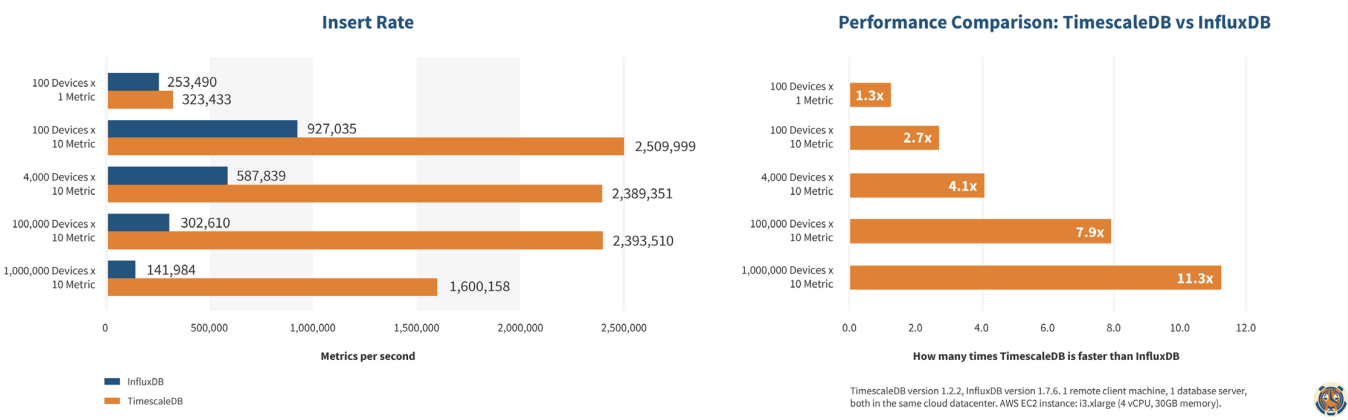
\includegraphics{obrazky-figures/db_comparisson.PNG}
    }
  \caption{Porovnání InfluxDB a TimescaleDB v~počtu vložených bodů za vteřinu na jednom uzlu \cite{InfluxVsTimescale}.}\label{pic:timescaleComparisson}
\end{figure}

%\section{Rozhraní pro komunikaci s úložišti}

\chapter{Návrh systému}\label{kap:design}
V~této kapitole je popsán návrh systému pro sběr, zpracování, vyhodnocení a zobrazení dat z~různých senzorů umístěných na průmyslových strojích.

Hlavními požadavky na systém je jeho snadná škálovatelnost, rychlost a modularita. Požadavky vychází ze zkušeností partnerské firmy s~jejich vlastním systémem. Škálovatelností je myšlena možnost rychlého nasazení nových jednotek se senzory a možnost jednoduchého rozšíření výpočetní síly serverové části, aby byla schopná efektivně zpracovávat data od různého množství jednotek. Modularitou systému je míněna možnost snadné výměny jednotlivých částí bez hlubších zásahů do programové části. Například změna úložiště dat, možnosti nasazení různých implementací jednotek, změna komunikačních protokolů a podobně. Systém by také měl být schopný zpracovávat data v~reálném čase a dostupnost uložených dat by měla být okamžitá.

\begin{figure}[h]
  \centering
  \scalebox{0.40}{
        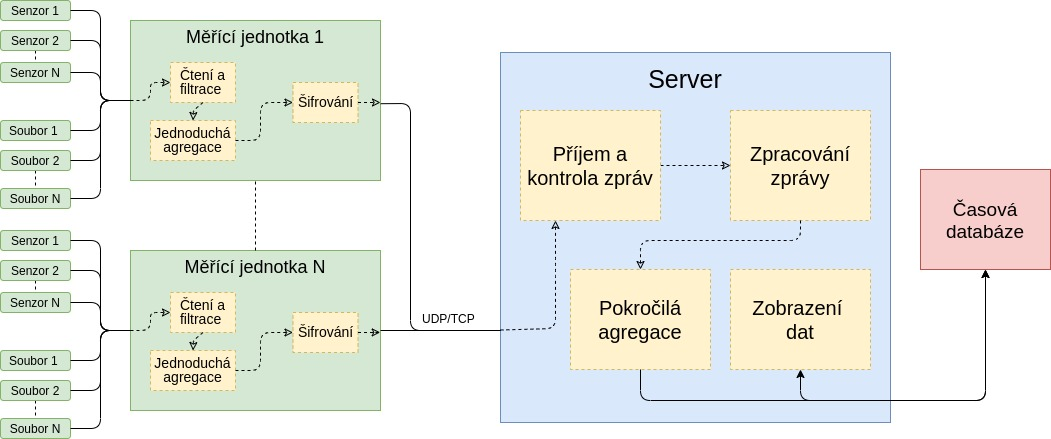
\includegraphics{obrazky-figures/Scalable_platform.jpg}
    }
  \caption{Zjednodušené schéma systému pro sběr, zpracování, vyhodnocení a zobrazení dat.}\label{pic:basic_design}
\end{figure}

Na obrázku \ref{pic:basic_design} je zobrazeno jednoduché schéma navrženého systému. Systém obsahuje měřící jednotky, které čtou data o~pevně nastavené vzorkovací frekvenci z~připojených senzorů, nebo v~případě testování ze souborů. Měřící jednotka kromě čtení provádí filtrování vstupních dat (například snížení vzorkovací frekvence). Vyfiltrovaná data jsou následně agregována jednoduchými, rychlými algoritmy. Po dokončení agregace jsou data zašifrována a pomocí protokolu UDP odesílána na server. Měřící jednotka je též schopná posílat na server neupravené bloky hodnot obsahující důležité úseky měření pro pokročilejší zpracování dat na serveru. Tato data jsou odesílána přes protokol TCP. Data agregovaná na jednotce slouží pro detekci fatálních poruch a sledování vytížení strojů. Tyto hodnoty mohou být využity pro spouštění odesílání nezpracovaných dat. Neagregovaná data zpracovávána serverovou částí neslouží k~detekci poruch, ale jejich predikci. Partnerská firma k~vypracování této práce poskytla software pro zpracování těchto hodnot a prototyp zařízení pro sběr dat ze senzorů vibrací a teploty. Návrh programové části pro měřící jednotku je ovlivněn vlastnostmi tohoto prototypu.

Zprávy přijímá serverová část. O~příjem se starají dva programy -- jeden pro zpracování UDP zpráv obsahující filtrovaná, agregovaná data a druhý pro příjem TCP zpráv s~neupravenými hodnotami. Programy zprávy dešifrují a provedou jejich kontrolu. Bloky neupravených dat jsou ukládány ve formátu TDMS\footnote{tdms -- Technical Data Management Streaming File} na úložiště pro pokročilé zpracování. Soubory slouží i jako záloha. Více informací k~formátu TDMS a účelu těchto dat se nalézá v~sekci \ref{subsec:tcp_server_design}. Hodnoty z~UDP zpráv, které jsou již předzpracované procházejí pokročilou agregací (pokud je to nutné). Následně jsou zapsány do časové databáze. Pokud tyto hodnoty překročí určitou hodnotu je uživatel či správce notifikován.

%popsat tdms soubory a jejich funkci do sekce k tcp serveru

\section{Měřící jednotka}
Měřící jednotka partnerské firmy na které byl vyvíjen software pro sběr a zpracování dat se skládá z~mini počítače Raspberry Pi verze 3b (dále jen RPi) a rozšiřující desky. Partnerskou firmou vyvinutá deska je k~RPi připojena přes GPIO (General-Purpose Input/Output) piny. Deska obsahuje ve starší verzi čtyři vstupy pro senzory vibrací a v~novější verzi i tři konektory pro snímání teploty. Návrh softwaru pro jednotku, jehož schéma je možné vidět na obrázku \ref{pic:unit_design}, je určen právě pro počítač RPi a je ovlivněn jeho parametry. Návrh také počítá s~připojením starší verze desky s~možností připojení čtyř senzorů vibrací, protože novější verze desky nebyla k~dispozici pro testování. Měřící jednotka běží na operačním systému Raspbian, který je linuxovou distribucí speciálně upravenou pro RPi.

RPi bylo zvoleno z~důvodu snadné dostupnosti, nízké ceny, výkonu a hlavně kvůli jeho rozšířenosti a velké komunitě. Pro RPi a linuxovou distribuci Raspbian existuje mnoho knihoven, které usnadňují implementaci komunikace s~připojenými periferiemi přes výstupní piny. 


\subsection{Čtení a filtrování dat}
Hlavní částí návrhu jednotky je program \textit{RawDataParser}, který se skládá ze dvou částí -- procesu pro čtení dat (\textit{Reader}) a procesu pro filtrování dat (\textit{Filter}). Hodnoty ze senzorů vibrací poskytuje analogově digitální převodník ADS131A04 od výrobce Texas Instruments. AD převodník je umístěný na rozšiřující desce a s~RPi komunikuje přes sériové periferní rozhraní (dále jen SPI). Proto program pro čtení dat podporuje komunikaci přes SPI, a z~důvodu testování má i podporu čtení dat ze souboru. AD převodník na desce vzorkuje data ze senzorů o~frekvenci až 128 kHz a proto software \textit{Reader} teoreticky zvládá číst až 512~000 hodnot za vteřinu (128 000 hodnot za vteřinu ze čtyř senzorů). Velikost jedné hodnoty je 24 b. Rozšiřující deska notifikuje RPi o~připravenost dat pro čtení pomocí sestupné hrany signálu pojmenovaném \textit{data ready} na nastaveném pinu. Čtení ze souboru nabízí stejnou možnost získávání dat o~nastavené vzorkovací frekvenci jako přes SPI.

Přečtená data jsou po časových úsecích zapisována do bloků sdílené paměti, ze které je čte filtrovací proces. Bloky jsou dva a vždy dochází k~zápisu do jednoho z~nich a čtení z~druhého. Takto navržené sdílení dat umožní, aby čtecí proces nečekal na uvolnění bloku sdílené paměti a tím nedocházelo ke ztrátě vzorků. Jakmile je časový úsek přečten filtrovacím procesem dojde ke snížení vzorkovací frekvence pomocí filtrů a takto zpracovaná data jsou umístěna do třetího bloku sdílené paměti pro agregační program. Neupravený časový úsek o~původní vzorkovací frekvenci je v~případě potřeby odesílána pomocí protokolu TCP na server pro účely výpočetně náročnějšího zpracování.

Jednotlivé procesy programu \textit{RawDataParser} jsou umístěny na izolovaných jádrech procesoru. Toto rozhodnutí bylo učiněno z~důvodu zvolené platformy a operačního systému. Nejedná se totiž o~\textit{real-time} operační systém. Z~toho důvodu není možné zajistit běh programu v~reálném čase, pokud jsou programy umístěny na jádrech s~více puštěnými procesy. Více k~této problematice se nachází v~\ref{sec:readAndFilter}.
 
\begin{figure}[h]
  \centering
  \scalebox{0.35}{
        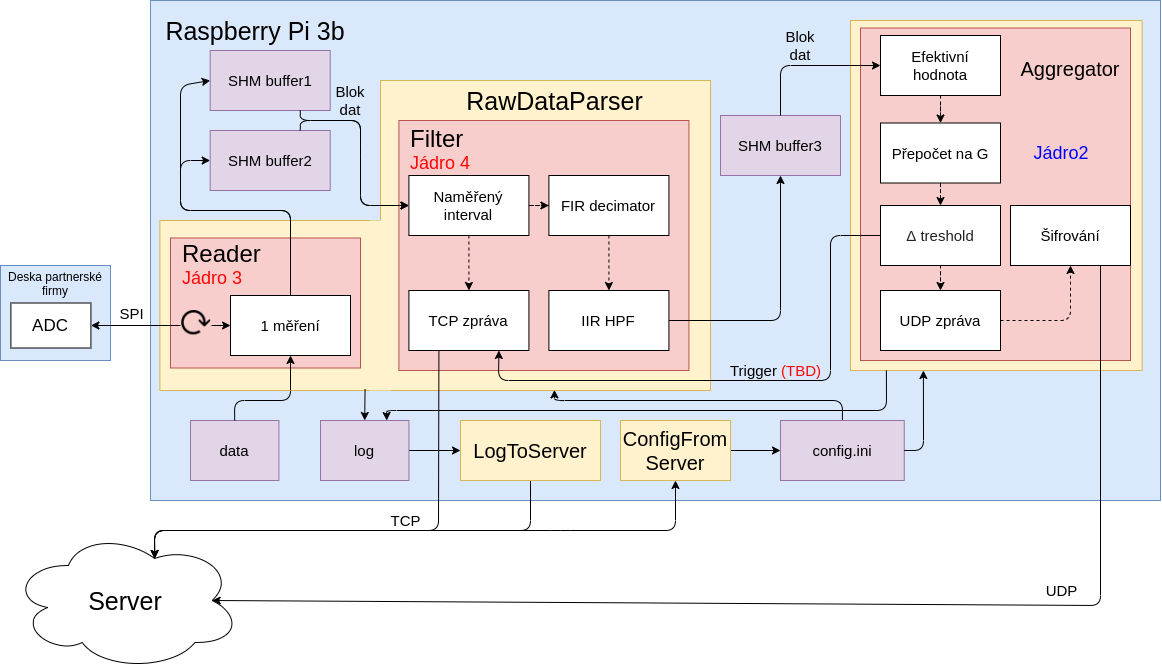
\includegraphics{obrazky-figures/unit.png}
    }
  \caption{Schéma softwaru měřící jednotky.}\label{pic:unit_design}
\end{figure}

\subsection{Agregace dat}
Jak již bylo zmíněno na začátku kapitoly, data agregovaná jednotkou slouží pro zobrazení vytížení stroje a případně i jako indikátor pro odesílání nezpracovaných dat na server. Návrh proto počítá s~triggerem, který upozorňuje filtrovací proces při překročení určité hodnoty. Tato hranice může být nastavena například na zapnutí stroje. Filtrovací proces po upozornění začne odesílat nezpracované bloky dat na server pomocí komunikačního protokolu přes TCP. Funkcionalita triggeru není kritická, ale slouží ke snížení síťové komunikace a potřebné výpočetní síly na serveru. V~případě kdy je sledovaný stroj vypnutý, nebude docházet ke zbytečnému odesílání dat k~pokročilému zpracovávání. Tato funkce ale může být překážkou pro stabilní zpracovávání dat není proto součástí výsledného systému. Nezpracovaná data jsou tedy vždy odesílána na server v~pravidelných intervalech nehledě na stav stroje.

Cílem agregačního programu je redukce dat se sníženou vzorkovací frekvencí předávaných přes sdílenou paměť programem pro čtení a filtrování na zhruba 1-100 vzorků za vteřinu. Toto rozpětí bylo vybráno proto, aby bylo možné zachovat nejdůležitější informace při velkých změnách v~měření. Díky tomu by při běžné činnosti nemělo docházet k~přílišnému zatěžování serverové strany obrovským množstvím hodnot. Za zvážení také stojí omezení zasílání agregovaných dat pokud je stroj nečinný. Neodesílání dat ve vypnutém stavu ale může zamezit sledování stroje v~reálném čase, protože aktualizace hodnot probíhá po delším časovém intervalu.

V~prvním kroku jsou data redukována na 100 vzorků za vteřinu. Tato redukce probíhá pomocí výpočtu kvadratického průměru popsaného v~sekci \ref{sec:vibrationAggregation}. V~dalším kroku dochází k~přepočtu hodnoty na zrychlení $g$ podle vzorce:
\begin{eqnarray}\label{eq:gravity}
  g & = & \frac{x_{out} - x_{rest}}{sensitivity}
\end{eqnarray}
kde $x_{out}$ je výstupní hodnota v~$mV$, $x_{rest}$ je klidová hodnota akcelerometru v~$mV$ a $sensitivity$ je citlivost senzoru v~$mV/g$. Citlivost je dohledatelná v~technické dokumentaci senzorů \cite{accelerationEq}. Po přepočtu na $g$ dochází v~dalším kroku k~zahození hodnot pomocí prahovací funkce hodnoty a času. Ponechány jsou pouze hodnoty, které se liší o~nastavený rozdíl či došlo k~překonání určeného časového intervalu od poslední uložené hodnoty. Po dokončení agregace je z~hodnot poskládána UDP zpráva. Zpráva je zašifrována a odeslána na server. Tato implementace zpracovává data ze senzorů vibrací. Konfigurační soubor ovšem obsahuje položku typ senzoru a v~případě připojení jiných typů senzorů je možné snadno doimplementovat jiný typ přepočtu na fyzikální veličiny či agregace.

%vypocet voltu http://www.ti.com/lit/ds/symlink/ads131a04.pdf


\subsection{Další programy a funkce}
Nejdůležitějším programem jednotky je \textit{RawDataParser} věnující se zpracováním dat. Kromě tohoto programu ovšem jednotka obsahuje i jiné podpůrné programy, skripty a soubory.

\subsubsection*{Instalační skripty}
V~rámci zjednodušení nasazení velkého počtu jednotek za co nejkratší možnou dobu je součástí návrhu sada instalačních skriptů, která automaticky při prvním zapojení inicializuje jednotku. Cílem sady skriptů je, aby pomocí spuštění jednoho skriptu na počítači s~připojenou SD kartou určenou pro RPi došlo k~vytvoření obrazu systému na kartě. Na kartu jsou nakopírovány všechny zbylé instalační skripty a potřebné soubory. Po vložení takto nachystané karty dojde ke kompletní instalaci a inicializaci všech částí softwaru jednotky, a to včetně určení unikátního ID, stáhnutí konfiguračního souboru ze serveru a spuštění samotného měření. Tato inicializace jednotky probíhá automatizovaně bez jakéhokoliv zásahu zvenčí.

\subsubsection*{Konfigurační soubor}
Konfigurační soubor poskytuje možnost jednoduchého nastavení jednotky. Obsahuje veškeré důležité informace pro běh programů a to je:
\begin{itemize}
    \item identifikátor jednotky obsahující unikátní sériové číslo procesoru RPi,
    \item zapnutí zápisu logů, cestu k~souborům s~logy, nastavení odesílání logů na server
    \item zdroj čtení, rychlost čtení, nastavení pinů, cesta k~zálohám a podobně,
    \item parametry pro agregaci hodnot,
    \item nastavení senzorů, jejich piny, zapnutí, citlivost a typ,
    \item IP adresy a porty k~serverům pro odesílání dat.
\end{itemize}
Konfigurační soubor je automaticky stahovaný ze serveru. Informace určené k~časté změně jsou na serveru uložené v~relační databázi jejíž návrh je popsán v~podsekci \ref{subsec:relation_db}. Upravovat pomocí databáze je možné nastavení agregace či parametry senzorů. Nastavení jako cesty k~zálohám či IP adresy serverů je možné změnit jen v~serverové aplikaci pro generování konfiguračního souboru. Jednotka periodicky zjišťuje, zda došlo ke změně konfiguračního souboru. Při změně dochází ke stažení nové konfigurace a restartu jednotky. Aktivní dotazování bylo zvoleno z~toho důvodu, že může nastat situace, kdy jednotku není možné notifikovat z~vnější sítě o~změně parametrů. Soubor má formát .ini. Formát .ini se člení na sekce záznamů a každý záznam obsahuje dvojici klíč, hodnota. Příklad obsahu souboru vypadá takto: 
\lstdefinelanguage{Ini}
{
    basicstyle=\ttfamily\small,
    columns=fullflexible,
    tag=[s]{[]},
    tagstyle=\color{blue}\bfseries,
    usekeywordsintag=true,
    morecomment=[l]{;},
    commentstyle=\color{gray}\ttfamily,
    alsoletter={=},
    ndkeywords={=},
    ndkeywordstyle=\color{green}\bfseries
}[html]
 \begin{lstlisting}[language={Ini}]
    ;aggreagation parameters
    [aggregation]
    delta = 10.2
    average = 80

    #server parameters
    [server]
    udp_ip: 255.255.255.255
    udp_port: 42
    \end{lstlisting}

\subsubsection*{Logování}
Chybové výstupy všech programů jsou ukládány do logovacích souborů. Logovací soubory jsou odesílány na server. Záznamy jsou ukládány v~následujícím formátu: \textit{[<časová značka>] [<název programu>] [<stav>] <zpráva>} Příkladem takového záznamu je: \textit{[2020-01-29 14:58:21.227] [Reader] [error] Unable to parse config file: missing frequency value}
%\subsection{Shrnutí návrhu jednotky a požadavky}
%ANO NEBO NE?

\section{Komunikační protokoly}\label{sec:comm_protocol}
UDP protokol je určený ke sledování dat s~co nejmenším možným zpožděním. To znamená časté zasílání menšího množství již agregovaných dat připravených k~přímému zápisu do databáze. Ztráta paketu nemá vliv na systém. Komunikační protokol je zobrazen na obrázku číslo \ref{pic:udp_protocol}. Protokol obsahuje verzi, unikátní identifikátor jednotky, časovou značku začátku měření a počet senzorů v~datové části. Hlavička senzoru je dlouhá 32 bitů. ID senzoru číslované od $0$ označuje index připojeného senzoru. Typ dat označuje jakým způsobem byla data zpracována a určuje do jaké databáze jsou vložena. Velikost označuje počet bajtů za hlavičkou senzoru obsahující hodnoty. Verze protokolu vyjadřuje v~jakém formátu jsou hodnoty odesílány. Maximální délka paketu byla zvolena 512 bajtů, což je minimální délka \textbf{datového bloku} paketu, kterou musí umět každé síťové zařízení zpracovat \cite{rfc791}. 

\begin{figure}[h]
\centering
\begin{subfigure}{.5\textwidth}
  \centering
    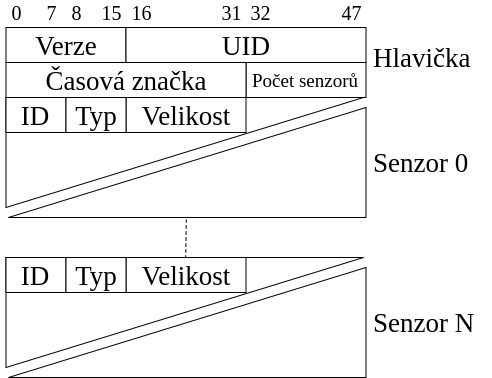
\includegraphics[width=.9\linewidth]{obrazky-figures/udp_paket.png}
    \caption{Schéma UDP paketu.}
  \label{pic:udp_protocol}
\end{subfigure}
\begin{subfigure}{.5\textwidth}
  \centering
    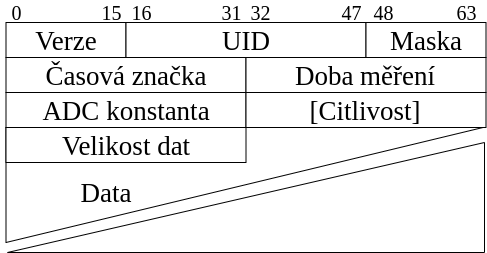
\includegraphics[width=.9\linewidth]{obrazky-figures/tcp_paket.png}
    \caption{Schéma TCP paketu.}
  \label{pic:tcp_protocol}
\end{subfigure}
\caption{Komunikační protokoly.}
\label{fig:test}
\end{figure}

Komunikační protokol založený na TCP slouží k~odeslání časového úseku nezpracovaných dat na pokročilé zpracování. Paket obsahuje oproti UDP zprávě navíc dobu měření ve vteřinách, ADC konstantu pro přepočet hodnot a pole citlivostí jednotlivých senzorů obsažených ve zprávě.



\section{Návrh serveru}
Serverová část systému je navržena tak, aby mohla fungovat pouze z~jednoho fyzického zařízení. V~případě potřeby je ovšem možné jednotlivé programy distribuovat na více serverů. Blokové schéma se nachází na obrázku \ref{pic:server_design}. Návrh obsahuje:
\begin{itemize}
    \item aplikace UDP a TCP serveru,
    \item relační databázi pro správu informací o~jednotkách,
    \item časovou databázi pro ukládání zpracovaných naměřených hodnot,
    \item datové úložiště pro zálohování nezpracovaných úseků měření ve formě TDMS souborů
    \item algoritmy partnerské firmy pro pokročilé zpracování TDMS souborů
    \item webovou aplikaci pro zobrazení grafů z~časové databáze
    \item program pro generování konfiguračních souborů z~databáze
    \item program pro přesměrování datového toku mezi více serverů.
\end{itemize}
Jednotlivé části návrhu jsou detailněji popsány v~následujících podsekcích. 

\begin{figure}[h]
  \centering
  \scalebox{0.44}{
        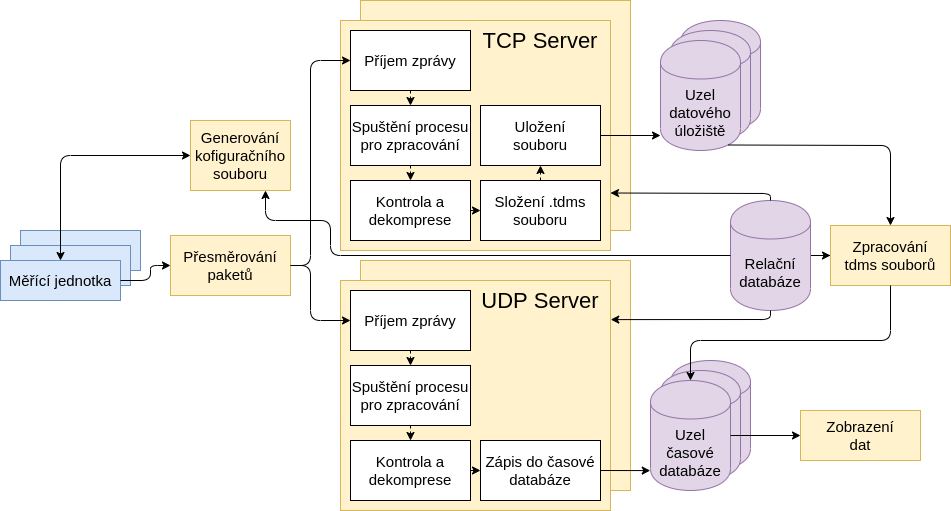
\includegraphics{obrazky-figures/server_design.png}
    }
  \caption{Schéma návrhu serverových aplikací a úložišť.}\label{pic:server_design}
\end{figure}

\subsection{UDP server}
Aplikace slouží pro příjem UDP zpráv obsahující zpracovaná data určená k~zápisu do časové databáze. Při příchodu zprávy dochází k~načtení verze protokolu a UID jednotky. Po načtení informací dochází k~dešifrování obsahu zprávy a k~zápisu hodnot do příslušných sérií v~časové databázi. Aplikace musí být schopna zpracovávat velké množství zpráv v~krátkém časovém úseku, po přijetí každé zprávy proto dochází ke spuštění nového procesu či vlákna, jehož účelem je zpracování zprávy.

\subsection{TCP server}\label{subsec:tcp_server_design}
Zasílání neupravených dat se děje z~důvodu, že RPi nemá dostatečný výkon pro aplikování pokročilých analýz nad daty o~vysoké vzorkovací frekvenci. Data agregovaná na jednotce jsou schopna detekovat poruchu při velké změně hodnot, ale právě agregací se ztrácí informace, které mohou indikovat blížící se poruchu. TCP server slouží k~přijímání bloků těchto dat a jejich zapsání do souborů ve formátu TDMS a uložení na datové úložiště. Formát byl zvolen z~důvodu využití aplikace partnerské firmy pro pokročilé zpracování dat. Tato aplikace je vytvořena v~programu LabView a vstupem jsou právě soubory ve formátu TDMS.

\subsection{Relační databáze}\label{subsec:relation_db}
Jednoduchá relační databáze slouží pro správu a nastavení jednotek, senzorů a přehled monitorovaných strojů. Schéma databáze je vidět na obrázku \ref{pic:relation_design}. Databáze obsahuje tabulky se společnostmi, jimi vlastněnými stroji a komponenty jednotlivých strojů. Senzory jsou připojené ke komponentům a tabulka senzorů obsahuje informaci o~citlivosti a zda je senzor zapojen. Senzory přísluší k~měřící jednotce, tabulka jednotky obsahuje zbylé informace potřebné pro vygenerování konfiguračního souboru.

\begin{figure}[h]
  \centering
  \scalebox{0.53}{
        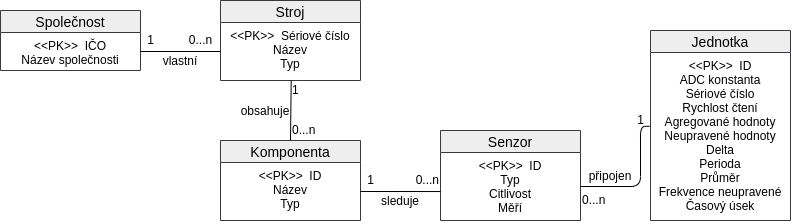
\includegraphics{obrazky-figures/Database.png}
    }
  \caption{Schéma návrhu relační databáze.}\label{pic:relation_design}
\end{figure}

\subsection{Časová databáze}
Tento typ úložiště slouží k~ukládání naměřených zpracovaných dat. Schéma na obrázku \ref{pic:time_series_design} obsahuje jednu databázi pro každou jednotku, jejíž název je unikátní ID jednotky. Jednotlivé databáze obsahují samotné časové série. Jméno časové série je odvozeno podle čísla senzoru, kterým byly hodnoty naměřeny, a podle způsobu, kterým byly zpracovány. Záznam je kombinací hodnoty a času. Pro zobrazování hodnot je využito grafické rozhraní zvolené databáze.

\begin{figure}[h]
  \centering
  \scalebox{0.60}{
        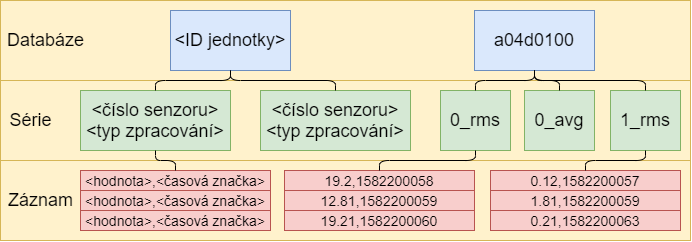
\includegraphics{obrazky-figures/time_series_design.png}
    }
  \caption{Schéma rozložení dat v~časové databázi.}\label{pic:time_series_design}
\end{figure}

\subsection{Ostatní programy a funkcionalita}
Součástí návrhu je program pro přesměrování paketů. Tento program umožňuje připojení více instancí TCP a UDP serverů. Pro tuto funkcionalitu je zvoleno již existující volně dostupné řešení a jeho využití v~systému je řešeno v~rámci testování. 

Další součástí je generování konfiguračního souboru. Program při zadání identifikátoru jednotky provede vygenerování konfigurace do souboru v~místě spuštění. Konfigurace jsou následně jednotkami staženy přes HTTP dotaz.


\chapter{Implementace}\label{kap:implementation}
Tato kapitola popisuje implementaci jednotlivých programů, popsaných v~návrhu. Kromě popisu implementace kódové části a ukázky nejzajímavějších částí kódu, se kapitola věnuje i postupu instalace a přípravy jednotlivých částí a návodům. Návody jsou umístěny v~přílohách.

\section{Server}
Jako operační systém pro server byla zvolena linuxová distribuci Ubuntu, respektive Ubuntu server. Zvolena byla z~důvodu její rozšířenosti, podpory a dostupnosti použitých knihoven. Některé příkazy použité při instalaci a přípravu serveru jsou v~umístěny v~příloze \ref{att:server_install}. 

\subsection{Příprava serveru}
Po instalaci operačního systému je vhodné povolit vzdálený přístup přes SSH (Secure Shel) pro možnost vzdálené správy. Zároveň je vhodné změnit port služby, aby bylo možné přistupovat k~více zařízení v~jedné síti přes SSH z~internetu a z~bezpečnostních důvodů deaktivovat účet \textit{root}. Port je potřeba povolit a pro přístup z~vnější sítě je nutné nastavit na routeru přesměrování portu na daný server. Jednotlivé příkazy jsou vypsány v~\ref{att:ssh}. Veškeré použité knihovny a příkazy k~jejich instalaci jsou v~příloze \ref{att:server_libs}.

\subsection{Časová databáze}
Při instalaci a nastavení časové databáze IfluxDB a webového rozhraní Chronograf bylo postupováno podle oficiální dokumentace\footnote{https://docs.influxdata.com/}. Po instalaci je vhodné upravit nastavení v~konfiguračním souboru \textit{/etc/influxdb/influxdb.conf}. V~souboru je nutné nastavit IP adresu, port a zapnout HTTP API s~autorizací. V~konfiguračním souboru lze nastavit i zálohování, dobu uchovávání dat a podobně. InfluxDB ukládá a čte data z~velkého množství souborů a proto je nezbytné zvýšit limit otevřených souborů pro proces. Pokud se neprovede zvýšení limitu, tak se databáze po vložení určitého množství dat stane nespustitelnou. Nespustitelnou zůstane až do navýšení limitu, protože nedokáže otevřít veškeré požadované soubory. Pro zvýšení limitu je potřeba v~souboru \textit{/etc/systemd/system/influxd.service} upravit nebo přidat řádek \textit{LimitNOFILE=infinity}. Dále je nezbytné v~souboru \textit{/etc/security/limits.conf} upravit limity pro uživatele a do terminálu zadat příkaz \textit{sudo sysctl -w fs.file-max=65000} a následně restartovat počítač.  Zvýšení limitu lze zkontrolovat příkazem \textit{grep files /proc/<influxdb pid>/limits}. Pokud se zvýšení provedlo, je hodnota limitu vyšší než jeden milion.

V~dalším kroku je potřeba vytvořit účty a tím zamezit přístupu k~databázi bez hesla. Do časové databáze se v~terminálu připojuje příkazem \textit{influx -username <username> -password <password>}, pokud není vytvořen žádný účet není nutné použít parametry účtu a hesla. Administrátorský účet se vytváří pomocí příkazu \textit{CREATE USER <username> WITH PASSWORD '<password>' WITH ALL PRIVILEGES}. Jednotlivé aplikace přistupující k~databázi mají své vlastní účty s~nezbytnými právy. 

Pro zobrazování dat z~databáze je využita webová aplikace Chronograf dostupná s~databází Influx. Aplikace je určena pouze pro lokální zobrazování dat a přístup do Chronografu nelze omezit pomocí přihlašovacích údajů. Přihlašovací údaje k~databázi má uloženy globálně pro všechna připojení. Z~důvodu testování je vytvořen pro aplikaci účet s~právy pro čtení, aby bylo umožněno k~zobrazení dat přistupovat i mimo lokální síť. Při každém vytvoření nové databáze je potřeba jednotlivým uživatelským účtům (mimo administrátorké účty) přiřadit práva k~nové databázi. Z~toho důvodu byl vytvořen skript \textit{privileges.sh}, který automaticky jednotlivým účtům přidá určená práva k~datovým databázím s~názvem ve formátu \textit{dat\_<UID>}, a tím usnadní přidávání nových databází. Skript je umístěn na přiloženém médiu. Chronograf je po spuštění dostupný pomocí lokálních webových stránek na portu $8888$. Pro zobrazení dat je nutné se připojit pomocí účtu vytvořeném v~InfluxDB. Pro přístup k~Chronografu mimo lokální síť, je nezbytné na routeru nastavit přesměrování portu $8888$ na zařízení s~databází.

\subsection{Relační databáze}
Pro relační databázi byla zvolena MariaDB s~webovým rozhraním Adminer. Pro snadnější instalaci je na přiloženém médiu skript \textit{mariadb.sh}, který provede kompletní instalaci obou aplikací. Skript nainstaluje mariaDB, PHP, curl a webový server nginx. Dále vytvoří složku \textit{/var/www/html/sql} pro webové rozhraní Adminer. Do složky je stažena aplikace Adminer, dojde k~přidání informací o~webovém serveru do konfiguračního souboru \textit{/etc/nginx/sites-enabled/default} a \textit{/etc/hosts} a k~dalším nutným úpravám konfiguračních souborů nginx a PHP pro zprovoznění webové aplikace Adminer. Po instalaci mariaDB je přidán administrátorský účet (přihlašovací údaje lze nalézt ve skriptu) a služby jsou spuštěny. Webové rozhraní pro správu databáze je dostupné na portu $9999$. Databáze vytvořená podle návrhu \ref{pic:relation_design} je v~exportované podobě bez hodnot uložená na přiloženém médiu v~soubor \textit{bp\_mariadb.sql}.

\subsection{TCPServer}
Program se spouští s~argumenty \textit{-p <port>} pro nastavení portu na kterém má TCP server naslouchat a \textit{-v} pro výpis logů do konzole. Program nevyužívá žádný konfigurační soubor. Pro logování je využita knihovna spdlog\footnote{https://github.com/gabime/spdlog}. Knihovna se skládá pouze z~hlavičkových souborů a není proto nutná její instalace. Ukládání logů rozdělených na informační a chybové se provádí do několika rotujících souborů o~maximální velikosti 5 MB. Po spuštění provede program inicializaci soketu a čeká na připojení. Při navázání spojení od klienta dojde k~vytvoření nového procesu. Původní proces čeká na připojení dalšího klienta a nově vzniklý proces provede příjem a zpracování zprávy. Při příjmu dojde nejdříve k~uložení hlavičky paketu do struktury \ref{list:tcp_header}. Po načtení hlavičky se provede alokace ukazatele dat \textit{data} na velikost \textit{dataSize} a k~příjmu naměřených hodnot. 
\begin{lstlisting}[style=c++, caption={Struktura pro příjem TCP zprávy.}, label={list:tcp_header}]
#define NUMBER_OF_CHANNELS

#pragma pack(push, 1)
struct TCPMessage{
    /* Header */
    uint16_t version;
    uint32_t uid;
    uint16_t channelMask;
    uint32_t timestamp;
    uint32_t duration;
    float adcConstant;
    float sensitivity[NUMBER_OF_CHANNELS];
    /* Data */
    uint32_t dataSize;
    uint8_t *data;
};
#pragma pack(pop)
\end{lstlisting}
Data TCP zprávy ve formě struktury jsou zpracována třídou \textit{Message}. Třída z~políčka \textit{channelMask} vyčte, které kanály jsou obsaženy ve zprávě a zkontroluje velikost dat a informace v~hlavičce. Pokud je zpráva poškozená, dojde k~zaznamenání chyby a zahození zprávy. Po zpracování je instance třídy \textit{Message} zastřešující přijatá data předána třídě \textit{TDMSFile}, která vytváří strukturu souboru ve formátu \textit{tdms}. Formát souboru se skládá ze tří částí: 
\begin{itemize}
    \item hlavička zvaná \textit{Lead In} obsahující informace o~verzi, velikosti dat a podobně,
    \item sekce \textit{Meta Data} s~informacemi o~jednotlivých kanálech a
    \item část \textit{Raw Data} s~daty z~kanálů uložených po blocích \cite{tdmsFileFormat}.
\end{itemize}
V~době psaní této práce nebyla k~dispozici žádná knihovna pro operační systém Linux a programovací jazyk C++, která by tvorbu těchto souborů umožňovala. Vytvořená třída \textit{TDMSFile}, starající se o~tvorbu souboru, neobsahuje plnou funkcionalitu pro práci se soubory, je totiž určena pouze k~vytvoření souboru s~pevně danou strukturou. Tato vlastnost umožnila třídu velice zjednodušit. Příkladem zjednodušení je tvorba hlavičky, která má pevnou délku a jediné části, u~kterých dochází ke změně je velikost a offset dat. Funkce pro zápis hlavičky do souboru vypadá následovně:
\begin{lstlisting}[style=c++, caption={Funkce pro zápis hlavičky tdms souboru.}]
#define TOC_MASK 0x0000000e
#define TDMS_VERSION 0x00001269

void TDMSFile::writeLeadIn() {
    uint32_t tocMask = TOC_MASK;
    uint32_t versionNumber = TDMS_VERSION;
    //first 4 bytes is TDSm tag
    fwrite("TDSm", sizeof(uint8_t), 4, tdmsFile);
    //4 bytes ToC mask
    fwrite(&tocMask, sizeof(uint32_t), 1, tdmsFile);
    //4 bytes version number
    fwrite(&versionNumber, sizeof(uint32_t), 1, tdmsFile);
    //8 bytes content length without lead in length
    fwrite(&dataLen, sizeof(uint64_t), 1, tdmsFile);
    //8 bytes raw data offset without lead in length
    fwrite(&rawDataOffset, sizeof(uint64_t), 1, tdmsFile);
}
\end{lstlisting}

\textit{Meta Data} obsahují informace o~kanálech nezbytné ke zpracování dat jako citlivost, konstanta AD převodníku a podobně. Některé údaje této části jsou opět neměnné. Naměřené hodnoty jsou do souboru zapsané po blocích ve formě 32b celočíselných hodnot. Název souboru obsahuje identifikátor jednotky a časovou značku počátku měření hodnot. Po vytvoření souboru dojde k~ukončení procesu pro zpracování. Součástí programu je i knihovna \textit{libzip} pro komprimaci souborů.

Zdrojový kód programu psaného v~C++ je umístěn na přiloženém médiu ve složce \textit{ServerSW/RawServer/}. Příkazy použité k~přeložení programu jsou v~příloze v~sekci \ref{att:compile}.
 
\subsection{UDPServer}
Program se opět spouští s~argumenty \textit{-p <port>} a \textit{-v} a je implementovaný v~jazyce C++. Součástí je i konfigurační soubor obsahující přihlašovací údaje do časové databáze. Program po spuštění zpracuje konfigurační soubor a vytvoří soket na daném portu. Při příjmu zprávy od jednotky uloží přijatá data do pole o~velikosti 512 bajtů, vytvoří instanci třídy \textit{Message}, která má na starosti zpracování zprávy a spustí nové vlákno pro zápis dat do databáze. Server je omezen v~počtu vláken které může spustit v~jeden okamžik, tato hodnota se nastavuje změnou makro konstanty \textit{NUM\_OF\_THREADS}. Hodnota by měla být nastavena podle výkonu zařízení na kterém je aplikace spuštěna. Nově spuštěné vlákno provede zpracování zprávy. Při zpracování zprávy je postupně plněna struktura \ref{code:udp} navržena podle komunikačního protokolu.
\begin{lstlisting}[style=c++, caption={Struktura dat zpracovaných z~UDP zprávy.}, label={code:udp}]
struct SensorData{
    uint32_t offset = 0;
    float value = 0;
};

struct Sensor{
    uint8_t sensorId = 0;
    uint8_t dataType = 0;
    uint16_t dataSize = 0;
    SensorData *data = nullptr;
};

struct UDPMessage{
    uint16_t version = 0;
    uint32_t uid = 0;
    uint32_t timestamp = 0;
    uint16_t numberOfSensors = 0;
    Sensor *sensor = nullptr;
};
\end{lstlisting}
Pro zápis dat do časové databáze Influx je využito HTTP komunikační rozhraní a knihovna curlpp. Vkládání hodnot probíhá přes HTTP požadavek obsahující přihlašovací údaje, upřesňující parametry a databázový příkaz. Metodou GET jsou předávány příkazy (\textit{write/read}) a parametry. Nezbytné parametry jsou: název cílové databáze \textit{db}, uživatelský účet \textit{u} a heslo \textit{p}. Příkaz může obsahovat i pokročilejší parametry jako \textit{precision}, který udává přesnost časové značky. Výchozí přesnost je v~nanosekundách. Databázový dotaz je předáván metodou \textit{POST}, je možné zapisovat několik hodnot najednou. Hodnoty jsou odděleny ukončením řádku a obsahují název časové série, hodnoty tagů a polí, naměřená data a časovou značku. Metoda pro zápis dat iteruje podle počtu senzorů a hodnot obsažených ve struktuře zprávy. Veškeré body zapíše do řetězce znaků a všechny body obsažené v~jedné UDP zprávě zapíše v~jednom dotazu. Příklad přidání jednoho bodu do SQL dotazu může vypadat následovně:
\begin{lstlisting}[style=c++, breaklines, caption={Přidání jednoho bodu do databázového dotazu}, label={code:httpapi}]
writeQuery += "sensor_" + sensorIndex + "_" + "rms_delta" + " value=" + data.value) + " " + data.timestamp"\n";
\end{lstlisting}
Pokud jde o~nultý senzor s~hodnotou 10.0 a časovou značkou 555555 nově přidaný řádek obsahuje \textit{sensor\_0\_rms\_delta value=10.0 555555}.

Zdrojový kód programu psaného v~C++ je umístěn na přiloženém médiu ve složce \textit{ServerSW/AggregationServer/}. Příkazy použité k~přeložení programu jsou v~příloze v~sekci \ref{att:compile}. Ke správnému fungování je potřeba dodat konfigurační soubor s~přihlašovacími údaji do časové databáze.

\subsection{Generování konfiguračního souboru}
Pro generování konfiguračního souboru ve formátu .ini slouží program \textit{ConfigGenerator}, umístěný na na přiloženém médiu ve složce \textit{ServerSW/ConfigGenerator/}. Program je vytvořený v~jazyce C++ a vyžaduje konfigurační soubor s~přihlašovacími údaji do relační databáze. Logování chyb opět probíhá pomocí knihovny spdlog. Program vyžaduje při spuštění argument obsahující identifikační číslo jednotky. Po spuštění se vygeneruje konfigurační soubor do aktuální složky. Ke komunikaci s~relační databází je využita knihovna \textit{mysqlcppconn}. Program obsahuje třídu \textit{ConfigGenerator}, která se stará o~generování konfiguračního souboru. Třída obsahuje tři veřejné metody:
\begin{itemize}
    \item \textit{void generateConfig();} získá všechny informace o~jednotce z~databáze, přesněji z~tabulek \textit{Unit} a \textit{Sensor},
    \item \textit{std::string getConfigString();} vrací řetězec znaků obsahující konfigurační soubor,
    \item \textit{void saveConfig(std::string path);} uloží konfigurační soubor, parametr \textit{path} udává cestu k~souboru.
\end{itemize}
Tato třída a její veřejné metody umožňují připojení k~například TCP serveru, který by na dotaz žádost jednotky odeslal konfigurační soubor. V~této práci je získání konfiguračního souboru řešeno přes HTTP dotaz a proto tento program pouze ukládá konfigurační soubor.

%zobrazeni csv a tdms pomoci python skriptu
%instalacni skript
%Struktura souboru je rozdělena do tří úrovní, nejvyšší úroveˇ
%cteni dat
%cteni ze souboru, popis pinu u rpi, vyvedeni data ready

%agregace

%sifrovani

\section{Jednotka}
Jak již bylo zmíněno, jednotka disponuje operačním systémem Raspbian. Jednotku není potřebné nijak připravovat, jediné co je třeba udělat pro její zprovoznění je vytvořit obraz systému na SD kartu pomocí instalačního skriptu. Jednotka obsahuje program pro čtení a filtrování, agregaci, stahování konfiguračního souboru a nahrávání logů na server.

\subsection{Instalační skripty}
Jedná se o~sadu skriptů a souborů sloužících k~téměř bezzásahovému zprovoznění jednotky. skripty jsou uloženy na přiloženém médiu ve složce \textit{ServerSW/SDCardInit/}. Jediný skript, se kterým pracuje uživatel je \textit{DiskCreator.sh}. Tento skript slouží k~překopírování všech potřebných souborů a ostatních souborů na SD kartu. Ve skriptu je potřeba upravit řádek \textit{mount /dev/sdd2 /mnt/sdcard} podle zařízení, na kterém je SD karta připojena. Skript kromě kopírování provede na kartě změnu inicializačního skriptu \textit{/etc/rc.local}. Tento skript se vykoná při každém spuštění. Do souboru přidá řádek spouštějící první instalační skript. Po prvním zapnutí jednotky s~nachystanou SD kartou je vykonán skript \textit{RTPatch.sh}, který ze souboru \textit{/proc/cpuinfo} zjistí verzi procesoru, podle ní zjistí verzi RPi a podle zjištěné verze aplikuje jeden z~předkompilovaných real-time patchů dostupných pro verze 3b, 3b+ a 4b. Po aplikaci patche je nutný restart, po kterém se spustí skript \textit{init.sh}. Další skript provede postupně:
\begin{itemize}
    \item spuštění SSH,
    \item instalaci knihoven,
    \item inicializaci watchdogu,
    \item stažení a překlad programů z~git repozitáře,
    \item nastavení programů jaky systémové služby,
    \item přidání skriptů do služby crontab pro jejich periodické spouštění,
    \item smazání nepotřebných zdrojových souborů a
    \item a finální restart jednotky.
\end{itemize}
Po finálním restartování je stažen konfigurační soubor a jednotka začíná měřit a odesílat data.

Skript pro kopírování souborů se spouští příkazem \textit{sudo bash ./DiskCreator.sh}. Na SD kartě musí již být vytvořen obraz operačního systému. Obraz operačního systému Raspbian Buster Lite\footnote{https://www.raspberrypi.org/downloads/raspbian/} lze vytvořit například pomocí aplikace balenaEtcher\footnote{https://www.balena.io/etcher/}. Následně stačí jednotku připojit k~internetu, vložit SD kartu a jednotka do pár minut začne měřit a odesílat data na server. 

\subsection{Čtení a filtrování dat} \label{sec:readAndFilter}
Čtení a filtrování dat provádí jeden program spouštějící dva procesy. Každý proces má alokované jedno fyzické jádro procesoru, které není k~dispozici operačnímu systému. Problémem zvolené platformy je, že systém neběží v~reálném čase a uživatel nemá plnou kontrolu nad vykonáváním programů. To by mohlo způsobit vynechávání velkého množství vzorků při čtení dat o~vysoké vzorkovací frekvenci. Alokace jader a instalace preemptivního real-time patche\footnote{https://wiki.linuxfoundation.org/realtime/start} pro kernel z~velké části řeší problém zvolené platformy. Alokace jader se provádí při inicializaci jednotky a to přidáním parametru \textit{rootwait/isolcpus=2,3 rootwait} souboru \textit{/boot/cmdline.txt}. Při pouštění programu je potřeba říci systému, na jakých jádrech a s~jakou prioritou má program spustit. Příklad spuštění vypadá následovně:
\begin{lstlisting}[language=bash, breaklines]
 $ sudo taskset -c 2,3 chrt -f 99 nice -n 20 <program> <program arguments>
\end{lstlisting}
Příkaz \textit{taskset -c 2,3} zbůsobí spuštění programu na jádrech $2$ a $3$, příkaz \textit{chrt -f 99} nastaví plánování procesu FIFO (First In First Out) a na nejvyšší prioritu (hodnota $99$). Příkaz \textit{nice -20} opět nastavuje nejvyšší možnou prioritu procesu.

Po spuštění programu dojde k~načtení konfiguračního souboru ve formátu .ini do struktury \textit{Config}. K~zjednodušení parsování konfiguračního souboru je využita knihovna \textit{INIReader.h}\footnote{https://github.com/benhoyt/inih}. Po načtení konfiguračního souboru je inicializována statická třída pro logování využívající stejnou knihovnu spdlog jako serverové aplikace a provede se vytvoření nového procesu. 

Původní proces se stará o~čtení dat z~nastaveného rozhraní. Proces si vytvoří instanci třídy pro čtení. Třídy pro čtení jsou vytvořené dvě, jedna pro čtení ze souboru a druhá pro čtení z~SPI. Obě třídy implementují stejné rozhraní a je tedy možné měnit jejich instance. K~naslouchání signálu \textit{data ready} a komunikaci přes piny pomocí SPI ve stejnojmenné třídě je využita knihovna bcm2835 psaná v~jazyce C a je využitelná na všechny verzi RPi. Knihovna poskytuje přístup k~pinům a dalším vstupně-výstupním zařízením a službám jako je SPI nebo I$^2$C. Třída obsahuje dvě veřejné metody, jednu pro inicializaci spojení a druhou pro nekonečné čtení z~rozhraní. Tyto dvě metody jsou zděděny z~rozhraní \textit{InterfaceReader}. Při inicializaci dochází k~nastavení SPI a převodníku ADS131A04 podle dokumentace\footnote{http://www.ti.com/lit/ds/symlink/ads131a04.pdf} a vytvoření pojmenované sdílené paměti. Sdílená paměť a semafory zajišťující výlučný přístup ke sdílené paměti jsou realizovány knihovnou boost. Vytvořená sdílená paměť má velikost bloku dat určitého časového intervalu upřesněného v~konfiguračním souboru.

Vyčítání a odesílání dat provádí funkce \textit{void bcm2835\_spi\_transfernb(char *tbuf, char *rbuf, uint32\_t len)}. Hexadecimální hodnoty registrů použité pro nastavení převodníku jsou umístěny ve zdrojovém souboru \textit{Spi.h}. Hodnoty jsou připravené k~přenosu při klesající hraně signálu \textit{data ready}, a proto je využita z~knihovny funkce \textit{bcm2835\_gpio\_afen(int pin\_number)}, která při padající hraně signálu na daném pinu nastaví událost (nastaví bit v~registru). Získání dat probíhá aktivním čekáním na událost pomocí funkce \textit{bool bcm2835\_gpio\_eds(int pin)}. Po nastání události jsou data přenesena a zapsána do jedné ze dvou sdílených pamětí. Jakmile je sdílená paměť naplněna, provede se odemčení semaforu dané paměti a tím se povolí čtení filtrovacím procesem. Následně dojde k~uzamčení semaforu druhé paměti pro čtení a začne zápis do druhé sdílené paměti. Díky této implementaci je vždy dostupný jeden blok sdílené paměti jak pro zápis tak i čtení.

V~případě čtení ze souboru je dosaženo vzorkování na požadované frekvenci vyvedením hodinového signálu na volný pin. Tento pin je potřeba fyzicky propojit s~pinem nastaveným jako \textit{data ready}. Vyvedení hodinového signálu je provedeno za použití knihovny \textit{pigpio} funkcí \textit{void gpioHardwareClock(int pin\_number, int frequency)}. Naslouchání signálu a přenos hodnot probíhá stejně jako v~případě třídy SPI.

Filtrovací proces po uvolnění semaforu zkopíruje obsah paměti do bufferu a uloží čas měření. Data z jednotlivých senzorů jsou zpracována decimačním filtrem, a tím je snížena vzorkovací frekvence na 8000 Hz. Data se sníženou vzorkovací frekvencí jsou následně zapsána do jednoho ze dvou bloků sdílené paměti, který slouží pro výměnu dat mezi filtrovacím procesem a agregačním programem. Následně je zkontrolováno, zda přijatý blok měření má být odeslán ve formě TCP zprávy a pokud ano, jsou původní nefiltrovaná data odeslána přes TCP spojení. 


\subsection{Agregace dat}
Agregaci hodnot provádí program \textit{Reader} psaný v~C++. Program je umístěn na přiloženém médiu ve složce \textit{/UnitSW/Aggregation} a spouští se s~parametrem \textit{-p <path>} s~cestou ke konfiguračnímu souboru. Program pro logování využívá knihovnu spdlog.

Program po spuštění načte z~konfiguračního souboru do struktury veškeré informace. Po načtení konfigurace dojde k~vytvoření instance třídy \textit{Aggregation}, inicializuje ji a spustí agregaci. Při inicializaci je otevřena sdílená paměť pro čtení, semafory a je alokována paměť pro zpracovávaná data. Sdílená paměť musí být vytvořena již před spuštěním tohoto programu. Program data zpracovává po časových úsecích, jejichž velikost je daná v~konfiguračním souboru. Po získání bloku dat pro zpracování je zavolána metoda \textit{void calculateRMS();}, která přijatá data převede na zrychlení a z~bloku hodnot o~snížené vzorkovací frekvenci spočítá kvadratický průměr, jehož vzorec je v~\ref{eq:root_mean_square}. Metoda je zobrazená na \ref{code:rms}. Metoda v~každém kroku hlavní smyčky spočítá jednu hodnotu kvadratického průměru pro každý senzor. Počet vzorků, které jsou průměrovány do jedné hodnoty, je nastaveno v~konfiguračním souboru. Metoda vypočítané hodnoty ukládá do dvourozměrného pole bodů rozděleného podle senzorů. Počet bodů pro průměrování je ve výchozím stavu nastaven tak, aby po přepočtení na kvadratický průměr zbývalo 100 bodů měření z~každého senzoru. Po výpočtu kvadratického průměru je aplikován algoritmus $\Delta treshold$. První bod každého bloku je vždy uložen pro odeslání. Ostatní body ponechány pro odeslání v~případě, že rozdíl jejich hodnoty a hodnoty posledního uloženého bodu překračuje v~konfiguraci nastavený práh, nebo pokud bylo od posledního uloženého bodu zahozeno příliš bodů (časový práh opět nastavený v~konfiguračním souboru). Body pro odeslání jsou uloženy do jednorozměrného pole struktur \textit{DataPoint}. Struktura vypadá takto:
\begin{lstlisting}[style=c++, breaklines]
struct DataPoint{
    float value;
    uint32_t time;
    uint32_t timeOffset;
    uint8_t sensorNumber;
};
\end{lstlisting}
a obsahuje hodnotu bodu, unixovou časovou značku času, kdy byl bod naměřen ve vteřinách, časový ofset v~nanosekundách a index senzoru. Po zpracování celého bloku hodnot je pole ponechaných bodů předáno třídě \textit{UDPClient}, která z~bodů poskládá zprávu odpovídající protokolu \ref{pic:udp_protocol} a zprávu odešle na server. Po odeslání zprávy program čeká na další blok dat.

\begin{lstlisting}[style=c++, caption={Výpočet kvadratického průměru z~bloku dat několika senzorů.}, label={code:rms}]
void Aggregation::calculateRMS() {
    int rmsIndex = 0;
    for(int dataIndex = 0; dataIndex < valuesPerChannel; dataIndex += config.average){
        float valueSum[NUMBER_OF_SENSORS] = {0};
        for(int blockOffset = 0; blockOffset < config.average; blockOffset++){
            for(int channelIndex = 0; channelIndex < NUMBER_OF_SENSORS; channelIndex++){
                float valueInG = buffer[dataIndex + blockOffset + channelIndex*valuesPerChannel];
                valueInG *= config.adcConstant;
                valueInG *= config.sensorSensitivity[channelIndex];
                valueSum[channelIndex] += valueInG*valueInG;
            }
        }
        for(int sensorIndex = 0; sensorIndex < NUMBER_OF_SENSORS; sensorIndex++){
            rms[sensorIndex][rmsIndex] = sqrtf(valueSum[sensorIndex]/config.average);
        }
        rmsIndex++;
    }
}
\end{lstlisting}

\subsection{Ostatní programy a funkcionalita}
K~získání konfiguračního souboru ze serveru slouží skript \textit{getconfig.sh} umístěný na přiloženém médiu ve složce \textit{UnitSW/}. Konfigurační soubory jsou ze serveru získávány pomocí HTTP dotazu na portu $9999$. Skript si udržuje hlavičku HTTP dotazu získanou při předchozím stažení souboru obsahující informaci o~poslední změně souboru. Skript periodicky získává ze serveru nové informace o~souboru a pokud dojde na ke změně souboru na serveru (indikující změna políčka \textit{Last-Modified}), stáhne se nový soubor a restartuje se měření s~novými parametry. Hlavička HTTP odpovědi, ze které skript získává informace vypadá následovně:
\begin{lstlisting}[language=bash, breaklines]
HTTP/1.1 200 OK
Server: nginx/1.16.1 (Ubuntu)
Date: Thu, 19 Mar 2020 09:44:44 GMT
Content-Type: application/octet-stream
Content-Length: 832
Last-Modified: Thu, 19 Mar 2020 09:31:21 GMT
Connection: keep-alive
ETag: "5e733be9-340"
Accept-Ranges: bytes
\end{lstlisting}


\chapter{Testování}\label{kap:test}
Tato kapitola se věnuje testování nejen systému jako celku, ale i testování jednotlivých komponent. Kromě testování funkčnosti systému, je kapitola též zaměřena na zátěžové testy serverových aplikací. Do zátěžových testů patří například zjištění, do kolika jednotek jsou jednotlivé aplikace schopné zpracovávat data bez zahlcení. Další částí jsou testy programu pro balancování zatížení serverových aplikací. Ten umožňuje spuštění několika instancí TCP a UDP serveru na více zařízeních, a tím navýšit limit zpracovávaných zpráv. Kapitola je také věnovaná testování zabezpečení síťové komunikace mezi jednotkou a serverovými aplikacemi a komprimace odesílaných dat.

\section{Test instalačních skriptů a kompletní funkce systému}
Cílem tohoto testu je vyzkoušet správnou funkčnost instalačních skriptů. Při správném fungování by po přípravě microSD karty a databáze měla jednotka během pár minut bez jakéhokoliv zásahu začít měřit a naměřená data odesílat na server.

Tento test byl prováděn s~rozšiřující deskou ve verzi 1.0. Desky ve verzi 1.0 a 1.1 nedisponují unikátním identifikátorem a z~toho důvodu bylo zvoleno jako ID kombinace MAC adresy RPi a typu jednotky. Před inicializací jednotky je nutné jednotku v~databázi vytvořit a k~tomu je potřeba znát ID. Pro zjištění identifikátoru byla do RPi vložena karta s~neupravenou instalací operačního systému Raspian a spuštěn příkaz:
\begin{lstlisting}[language=bash, breaklines, label={code:uid}]
$ echo "c0$(cat /sys/class/net/eth0/address | tr -d ':' | tail -c 7)"
\end{lstlisting}
Tento příkaz na standardní výstup vypíše dvě hodnoty pro námi zvolený typ jednotky ($c0$) a posledních šest hodnot MAC adresy jednotky. V~případě testované jednotky to je $d2bdb4$. Do databáze je tedy přidána jednotka s~tímto ID. Následně jsou v~databázi vytvořeny čtyři senzory s~potřebnými parametry a pomocí programu \textit{ConfigGenerator} je vygenerován konfigurační soubor \textit{config}, jehož obsah je možné vidět na přiloženém médiu v~kořenovém adresáři. Před přidáním nové jednotky do systému musí být vytvořena i příslušná databáze v~časové databázi a uživatelským účtům musí být přidělena práva pomocí skriptu \textit{privileges.sh}. Po provedení těchto kroků je již serverová část připravena na provoz nové jednotky. Dalším krokem pro zprovoznění nové jednotky je vytvoření obrazu operačního systému Raspbian na kartě a spuštění skriptu \textit{SDCardInit.sh}. Jednotka s~připravenou kartou musí být před spuštěním připojena k~internetu pomocí ethernetového kabelu, jinak nedojde ke stažení knihoven a softwaru. Tímto je dokončena příprava na instalaci.

Jednotka s~připravenou kartou byla spuštěna v~11:48:21 a instalace byla dokončena v~12:15:15. Jednotka má nastavené dvouminutové zpoždění pro spuštění čtecích programů (zamezení restartovací smyčky způsobené možnou nestabilitou čtecího programu) a první agregované hodnoty byly tedy do databáze zapsány o~zhruba dvě až tři minuty později, viz obrázek \ref{pic:installsdf}. Na obrázku je možné vidět, že byly přijaty agregované hodnoty ze čtyř senzorů. K~jednotce nebyl připojen senzor, jedná se tedy pouze o~šum na analogovém vstupu.
\begin{figure}
  \centering
  \scalebox{0.21}{
        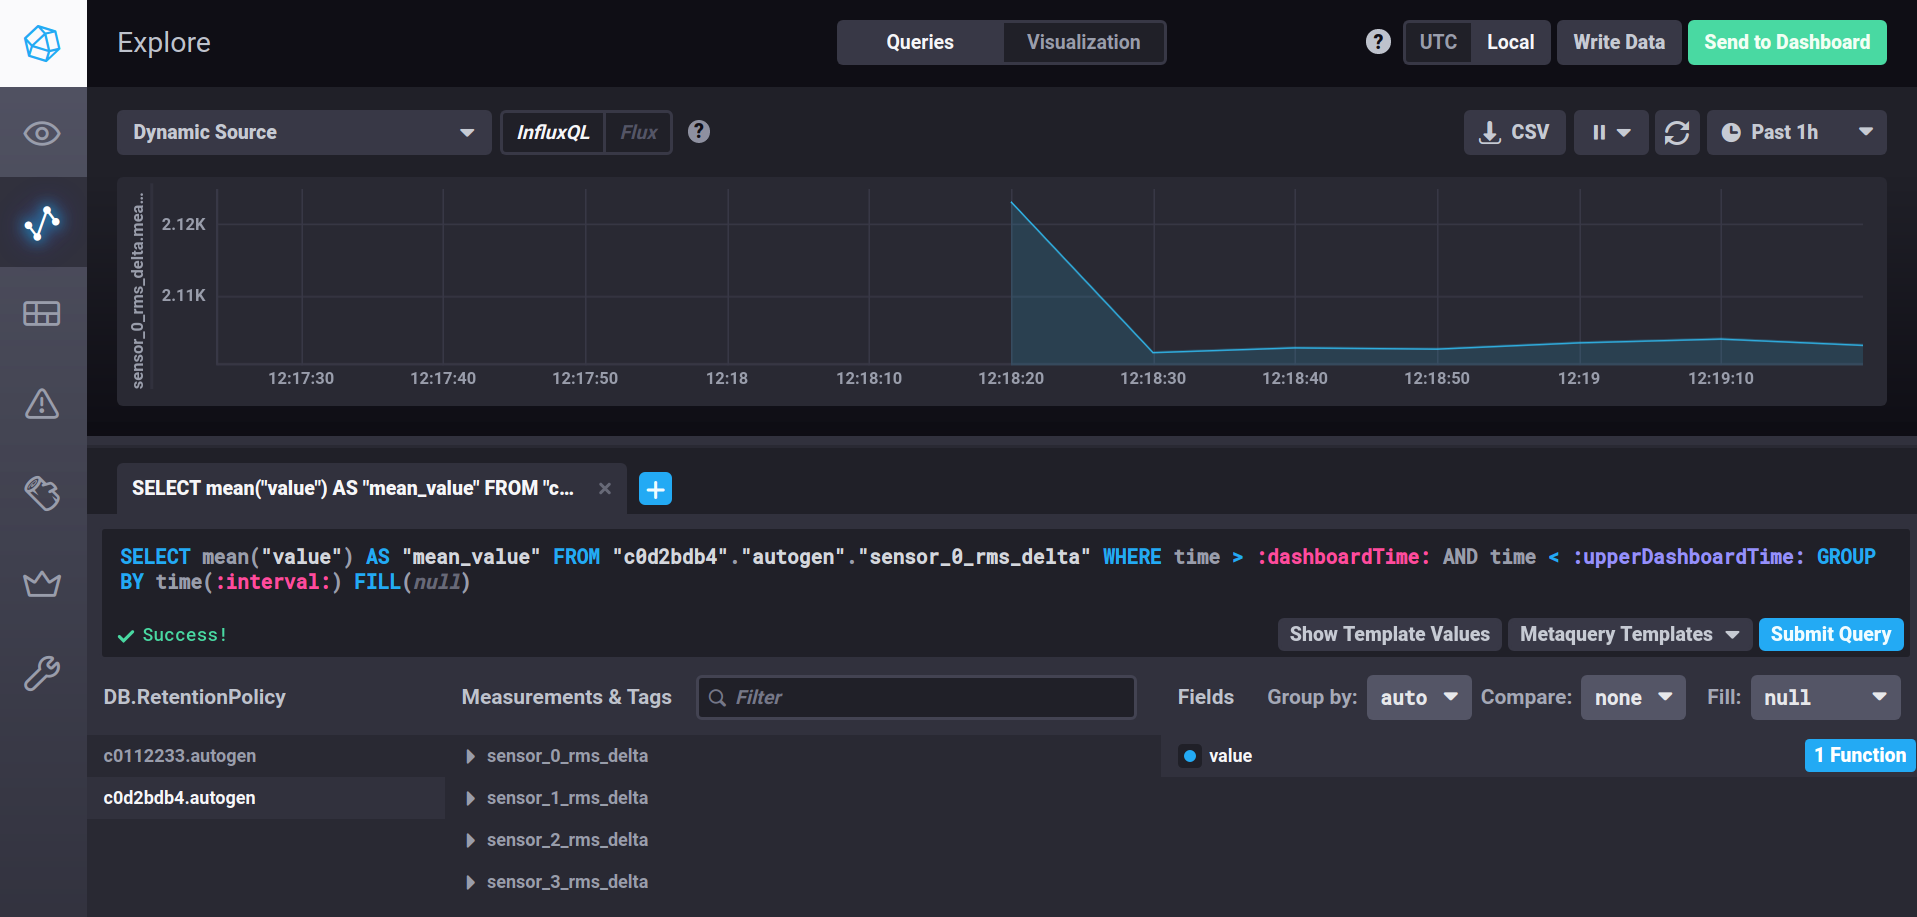
\includegraphics{obrazky-figures/influx_instal_data.png}
    }
  \caption{První přijatá data po dokončení instalace.}\label{pic:installsdf}
\end{figure}
Konfigurační soubor byl před spuštěním úspěšně stažen ze serveru. Na obrázku \ref{pic:htop} je vidět rozložení procesů na jednotlivých jádrech. Z~obrázku je patrné, že program \textit{Reader} využívá dvě procesorová jádra, která pro něj byla alokována. Proces využívající třetí jádro provádí čtení dat z~nastaveného rozhraní. Stoprocentní využití jádra způsobuje aktivní čekání na signál \textit{data ready}. Proces spuštěný na čtvrtém jádře aplikuje filtry na bloky dat získaných od čtecího procesu a využívá jádro průměrně na $50 \%$. Oba procesy mají RT prioritu. Agregační program je spuštěn na zbývajících jádrech společně se systémem.
\begin{figure}
  \centering
  \scalebox{0.30}{
        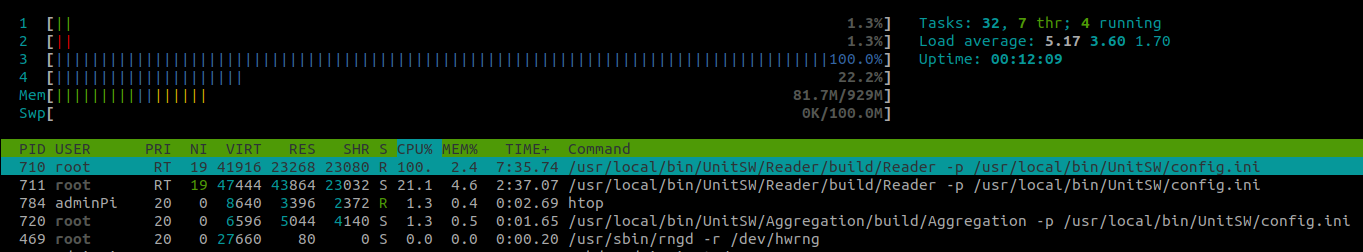
\includegraphics{obrazky-figures/htop.png}
    }
  \caption{Využití procesoru při čtení a rozložení procesů na jednotlivých jádrech.}\label{pic:htop}
\end{figure}
Soubory s~logy byly vytvořeny správně na nastavené cestě a obsahovaly informaci o~neúspěšném pokusu o~navázání TCP spojení. Při kontrole konfiguračního souboru byla objevena chyba v~IP adrese pro TCP server. IP adresa byla opravena na serveru a opravený soubor byl jednotkou během následujících pěti minut stažen a došlo k~restartování čtení a byla navázána i TCP komunikace viz obrázek \ref{pic:tcpinstall}. 
\begin{figure}
  \centering
  \scalebox{0.34}{
        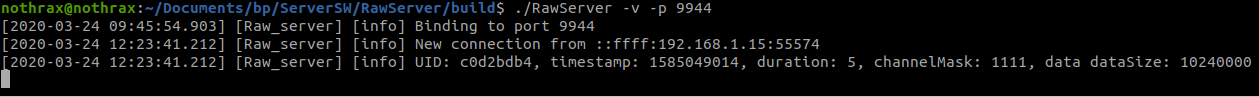
\includegraphics{obrazky-figures/raw_connection.png}
    }
  \caption{Informace o~příchozí zprávě na TCP server.}\label{pic:tcpinstall}
\end{figure}
Výstup instalačního skriptu je směřován do souboru \textit{install\_log.txt}. Tato vlastnost je důležitá pro kontrolu instalace. Pokud dojde při instalaci k~jakékoliv chybě, je možné záznam o~ní vyhledat právě v~tomto souboru. Soubor z~testovací instalace je přiložen v~kořenové složce na přiloženém médiu. Výstup skriptu byl zkontrolován a neobsahuje žádná chybová hlášení.

Tento test ověřil funkčnost bezzásahové inicializace jednotky a dobu nutnou k~jejímu zprovoznění. Čas potřebný pro zaměstnance pro přidání jednotky do databáze a přípravu instalační karty je zhruba deset minut a je zde prostor pro další urychlení. Například vytvořením jednoduchého uživatelského rozhraní, přes které by bylo možné na jednom místě jednoduše přidat jednotku do databáze a vytvořit její instalační kartu. Bezzásahová instalace jednotky trvala zhruba 27 minut a měření bylo zahájeno po 30 minutách. Tímto testem byla vyzkoušena i kompletní funkcionalita celého systému.

\section{Komprimace zpráv}
Cílem testu bylo porovnat kompresní algoritmy pro využití při odesílání neagregovaných dat a zvolit nejvhodnější algoritmus pro implementaci v~jednotce. TCP zprávy obsahující nezpracovaná data mohou nabývat velikosti až několik MB. Z~toho důvodu je vhodné využít rychlý kompresní algoritmus pro snížení velikosti, který může jednotka využívat v~reálném čase. Pro test byly vybrány běžně využívané kompresní algoritmy \textit{deflate}, \textit{LZO} (Lempel–Ziv–Oberhumer), \textit{LZMA} (Lempel-Ziv-Markov-Chain), \textit{BZip2} a metoda \textit{Delta compression} popsaná v~\ref{sec:delta}. Algoritmy byly testovány na nezpracovaných historických datech dodaných partnerskou firmou v~binární podobě. Algoritmy byly testovány na souborech o~velikosti zhruba 500 kB, 3 MB a 10 MB. Testované soubory jsou umístěny na přiloženém médiu ve složce \textit{Testing/}. K~testování algoritmů \textit{deflate} a \textit{Delta compression} byl vytvořen program \textit{DataCompress}, umístěný ve stejné složce jako testované soubory. Ostatní algoritmy byly testovány pomocí skriptu \textit{compress.sh}, vytvořeného pro účely testu. Výsledky obsahuje tabulka \ref{tab:compress_test}.

\begin{table}[h]
    \begin{center}
        \begin{tabular}{|c|c|c|c|c|c|c|c|c|}
        \hline
        \multirow{2}{*}{alg.} & \multicolumn{2}{c|}{500kB}      & \multicolumn{2}{c|}{3MB}        & \multicolumn{2}{c|}{10MB}       \\ \cline{2-7} 
                                    & velikost{[kB]} & doba{[ms]} & velikost{[kB]} & doba{[ms]} & velikost{[MB]} & doba{[ms]} \\ \hline
        LZO                         & 222,0            & 2            & 1275,0           & 7            & 4,1              & 21           \\ \hline
        Delta                       & 212,1            & 24           & 1234,5           & 138          & 4,0              & 429          \\ \hline
        BZip2                       & 80,2             & 89           & 455,9            & 219          & 1,5              & 522          \\ \hline
        LZMA                        & 92,6             & 138          & 494,6            & 787          & 1,7              & 3201         \\ \hline
        Deflate                     & 108,8            & 438          & 612,5            & 2048         & 2,0              & 6669         \\ \hline
    \end{tabular}\caption{Výsledky testů kompresních algoritmů.} \label{tab:compress_test}
    \end{center}
\end{table}

Výsledky testu jsou seřazeny podle doby trvání komprese. Test ukázal, že algoritmus \textit{Deflate}, běžně využívaný knihovnou \textit{libzip}, je pro řešení naprosto nevhodný. Oproti ostatním algoritmům je doba potřebná pro kompresi až čtyřikrát vyšší a to s~horším kompresním poměrem. Nejlepšího kompresního poměru dosáhly algoritmy \textit{BZip2} a \textit{LZMA}. \textit{BZip2} je až šestkrát rychlejší než \textit{LZMA}, a proto pokud záleží na kompresním poměru, je nejlepší volbou. U~řešeného systému je ale velmi důležitá rychlost komprese, protože jednotka potřebuje provádět kompresi v~reálném časem, aby nedocházelo k~výpadkům. Algoritmus \textit{Delta} dosahuje zhruba 75\% úspory a lepší rychlosti než předchozí algoritmy. \textit{LZO} ovšem dosahuje stejného kompresního poměru při $10-20$ násobně kratší době. Tento algoritmus je tedy pro účely komprese implementován v~jednotce. 

\section{Propustnost serverů}
Cílem těchto testů je určit množství zpráv, které jsou UDP a TCP servery schopné přijmout za určitý čas. Určením limitu příchozích zpráv na server je možné vyvodit, kolik jednotek je možné obsluhovat jednou instancí. Množství zpráv, které jsou schopné aplikace zpracovat, se odvíjí i od výkonu zařízení na kterém jsou aplikace spuštěny a rychlosti připojení. Veškeré testy UDP a TCP serverů byly prováděny na počítači vybaveném čtyřjádrovým procesorem intel core i7 6700k, 32 GB RAM paměti. Síťová komunikace probíhala přes gigabitové spojení.

Pro účely testu byl vytvořen program \textit{MessageGenerator}, umístěný na přiloženém médiu ve složce \textit{Testing/}. Program po spuštění generuje podle nastavení buď UDP nebo TCP zprávy. Program vytváří několik vláken. Každé vlákno představuje jednu virtuální jednotku, která v~nastavených intervalech odesílá zprávy. Program se spouští s~následujícími parametry:
\begin{itemize}
    \item \textit{-m <UDP|TCP>} volba režimu,
    \item \textit{-u <počet jednotek>} počet jednotek,
    \item \textit{-f <milisekundy>} čas v~milisekundách mezi zprávami od jednotky,
    \item \textit{-p <port>} port cílového zařízení,
    \item \textit{-a <IPv4>} IPv4 adresa cílového zařízení.
\end{itemize}
Generované zprávy mají formát popsaný v~\ref{sec:comm_protocol}. UDP zprávy jsou plně zaplněny do velikosti 512 B. TCP zprávy obsahují měření o~délce deseti vteřin ze čtyř senzorů o~vzorkovací frekvenci 128000 Hz. Každé vlákno, neboli virtuální jednotka, má přiřazen speciální identifikátor, například \textit{f0010012}. \textit{f} označuje test, následující tři hodnoty \textit{001} určují číslo testu a poslední čtyři hodnoty udávají index virtuální jednotky. 

\subsection{UDP server}
První test UDP serveru ověřoval funkčnost programu pro generování zpráv. Pro účely testu byly v~časové databázi vytvořeny jednotky \textit{f0010000} a \textit{f0010001} a pomocí skriptu \textit{privileges.sh} byla přidána práva jednotlivým uživatelským účtům. Cílem testu bylo do databází těchto dvou jednotek vložit sto dvacet hodnot ke každému senzoru z~deseti zpráv. Po spuštění programu byl skutečně do databáze pod každý senzor vložen požadovaný počet hodnot. Každá zpráva je pro snadnější vyhodnocení v~databázi reprezentována jako jedna vteřina. Pokud se tedy pošle deset zpráv po 50 ms rozestupech, v~databázi jsou hodnoty roztaženy do deseti vteřin. Podobným způsobem byla otestována funkčnost na TCP serveru, ze tří zařízení bylo odesláno deset zpráv. Na serverové straně bylo vygenerováno třicet souborů. 

U~každého provedeného testu bylo potřeba pro všechna zařízení vyhodnotit počet přijatých zpráv a spočítat množství chybějících zpráv. Jelikož by u~desítek zařízení bylo toto vyhodnocení velmi zdlouhavé, byl vytvořen vyhodnocovací skript \textit{evaluateLoadTest.sh}. Vstupním parametrem skriptu je \textit{-u <jednotek>} pro počet zařízení a \textit{-d <čas>} určující dobu mezi zprávami v~milisekundách. Výstupem skriptu je soubor s~tabulkou obsahující informace o~počtu chybějících zpráv v~jednotlivých minutách u~všech zařízení. Příklad výstupu vyhodnocovacího skriptu pro deset jednotek s~jednou zprávou za vteřinu po dobu deseti minut je možné vidět na obrázku \ref{pic:load_verif_script}. Každý řádek představuje údaje týkající se jedné jednotky. První sloupec označuje ID jednotky, druhý sloupec celkový počet zpracovaných zpráv a celkový počet odeslaných zpráv. Každý další sloupec představuje jednu minutu testu. Pokud je ve sloupci hodnota 60/60 znamená to, že bylo přijato 60 zpráv a odesláno také 60 zpráv. Skript je umístěn na přiloženém médiu ve složce \textit{Testing/}. 

\begin{figure}[h]
  \centering
  \scalebox{0.34}{
        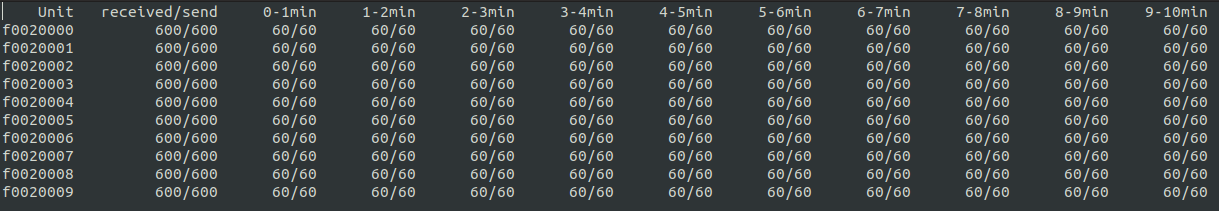
\includegraphics{obrazky-figures/output_test.png}
    }
  \caption{Ukázka výstupu vyhodnocovacího skriptu.}\label{pic:load_verif_script}
\end{figure}

Pro průběh každého testu bylo nutné vytvořit jednotlivé databáze, což je u~desítek zařízení velmi zdlouhavé. K~přidávání jednotek do databáze pojmenovaných podle pravidla zmíněného dříve byl vytvořen skript \textit{createTestDatabases.sh} umístěný ve stejné složce jako skript vyhodnocovací. Vstupními argumenty jsou počet jednotek \textit{-u <jednotek>} a číslo testu \textit{-t <číslo testu>}. Skript se pokusí před vytvořením databází smazat staré databáze se stejným názvem. 

Výsledky testů bez zabezpečení je možné vidět v~tabulce \ref{tab:graph_test_1}. Sloupec \textit{jednotek} udává počet virtuálních jednotek, \textit{zpoždění} stanovuje dobu mezi zprávami od jedné jednotky, \textit{délka t.} určuje dobu trvání testu, \textit{přijato} určuje v~procentech kolik odeslaných zpráv bylo přijato a \textit{zpráv/s} udává kolik zpráv dohromady UDP server obdržel každou vteřinu. Výstupy všech testů vygenerovaných vyhodnocovacím skriptem jsou na přiloženém médiu ve složce \textit{Testing/output/}. 

Prvních devět testů bylo určeno pro hrubý odhad maximálního limitu zpracovaných zpráv. Z~testů vyplývá, že UDP server zvládá bez problému zpracovat a zapsat do databáze sto zpráv za vteřinu. Při tisíci zprávách za vteřinu docházelo již k~1-4\% ztrátám. Při deseti tisících zprávách za vteřinu byla ztrátovost přes 90 \%. Tyto hodnoty naznačují, že maximální množství zpracovaných zpráv na testovaného zařízení je zhruba $950-980$ za vteřinu ze všech jednotek. 

Testy číslo 10, 11 a 12 sloužily k~přesnějšímu určení bezpečného limitu zpracovaných zpráv. Bezpečné množství, při které nedošlo k~žádné ztrátě, je zhruba 600 zpráv za vteřinu. Počet zpráv lze zvýšit zlepšením parametrů zařízení, na kterém je UDP server spouštěn. Je potřeba také brát v~potaz, že na stejném zařízení byla spuštěna i časová databáze. Maximální počet agregovaných hodnot, které je jednotka schopná vygenerovat ve verzi 1.0, je 400 hodnot za vteřinu ze všech senzorů. Jedna UDP zpráva protokolu používaného v~této práci pojme až 56 hodnot. Jednotka je tedy schopná vygenerovat maximálně 8 UDP zpráv za vteřinu. Testovaný UDP server bez zabezpečení zvládne zpracovávat data bez ztráty od 75 jednotek.

Testy 12 a 13 z~tabulky \ref{tab:graph_test_1} byly provedeny se zašifrovanými zprávami. Zprávy byly šifrovány pomocí operace XOR\footnote{https://teambi0s.gitlab.io/bi0s-wiki/crypto/xor/}. Šifrování funguje na principu bitového klíče, který je stejně dlouhý jako UPD zpráva. Klíč zná pouze serverová a klientská aplikace a na jednotku je dodán při její instalaci. Každý bit odesílané zprávy je změněn operací XOR s~odpovídajícím bitem klíče. Zpráva je následně odeslána a na serveru stejným způsobem dekódována. Jak je možné vidět v~tabulce, šifrování mělo vliv na množství zpracovaných zpráv. Už u~600 zpráv docházelo k~drobným výpadkům kolem 0,07 \%, snížení počtu zpráv na 500 za vteřinu tento výpadek vyřešilo.

Pokud by bylo potřebné zpracovávat data od více jednotek, je nutné využít více instancí serveru a program pro vyvažování zátěže testovaný v~\ref{sec:load_balancing}.

\begin{table}[h]
    \begin{center}
        \begin{tabular}{|c|c|c|c|c|c|}
        \hline
             č. testu & jednotek & zpoždění[ms] & délka t.[min]& přijato[\%] & zpráv/s\\ \hline
             $1$ & $1$ & $1000$ & $10$ & $100$ & $1$\\\hline
             $2$ & $10$ & $1000$ & $10$ & $100$ & $10$  \\\hline
             $3$ & $100$ & $1000$ & $10$ & $100$ & $100$  \\\hline
             $4$ & $1$ & $100$ & $10$ & $100$ & $10$  \\\hline
             $5$ & $10$ & $100$ & $10$ & $100$ & $100$ \\\hline
             $6$ & $100$ & $100$ & $10$ & $97,75$ & $1000$  \\\hline
             $7$ & $1$ & $10$ & $10$ & $99,99$ & $100$  \\ \hline
             $8$ & $10$ & $10$ & $10$ & $96,78$ & $1000$  \\ \hline
             $9$ & $100$ & $10$ & $10$ & $8,91$ & $10000$ \\ \hline
             $10$ & $90$ & $100$ & $10$ & $91,98$ & $900$ \\ \hline
             $11$ & $80$ & $100$ & $10$ & $95,85$ & $800$ \\ \hline
             $12$ & $60$ & $100$ & $10$ & $100$ & $600$ \\ \hline \hline
             $13$ & $60$ & $100$ & $10$ & $99,93$ & $600$ \\ \hline
             $14$ & $50$ & $100$ & $10$ & $100$ & $500$ \\ \hline
        \end{tabular}
        \caption{Výsledky zátěžových testů UDP serveru.} \label{tab:graph_test_1}
    \end{center}
\end{table}

\subsection{TCP server}
Pro testování TCP serveru bylo opět využito testovacího programu \textit{MessageGenerator}. Cílem testu bylo zjištění, od kolika jednotek je server schopný přijímat data. Výsledky testů jsou v~tabulce \ref{tab:graph_test_2}. Oproti předchozímu testu přibyl sloupec \textit{interval}, určující jak dlouhý časový úsek měření zpráva obsahuje. Během každého testu byly určitou dobu odesílány zprávy s~fixním zpožděním. K~zahlcení došlo, pokud server po uplynutí určené doby nezpracoval požadovaný počet zpráv. 

Počet maximálního množství jednotek je určen několika faktory. Závisí na délce zprávy, kterou jednotka odesílá, a také jak často tyto zprávy odesílá. TCP protokol a implementace jednotky umožňují jako nejnáročnější možnou kombinaci nastavení zprávy obsahující jednu vteřinu měření odesílané každou vteřinu, tzn. téměř nepřetržitý datový tok od každé jednotky. Toto nastavení by ovšem vedlo k~rychlému zahlcení serverové aplikace a mohlo by způsobit výpadky v~měření. Proto je jako nejhorší možný scénář zvoleno nastavení měření o~délce deseti vteřin a odesílání všech dat. Testy 1, 2, 3 a 4 se zabývají právě touto situací. Z~výsledku lze odvodit, že TCP server je schopný zpracovávat data od 50 jednotek, které posílají veškerá naměřená data po deseti vteřinových úsecích (zhruba pět zpráv za vteřinu). 

Systém ovšem není koncipován na odesílání veškerých naměřených nezpracovaných dat, ale na odesílání intervalů nezpracovaných dat po určitém čase. Testy 5 a 6 vychází ze situace, kdy každá jednotka odesílá desetivteřinové úseky měření jednou za minutu. Podle dosavadních výsledků by server měl v~této situaci zvládat zpracovávat data až od 300 jednotek a test číslo 5 to potvrzuje.

\begin{table}[h]
    \begin{center}
        \begin{tabular}{|c|c|c|c|c|c|c|}
        \hline
             č. testu & jednotek & zpoždění[s] & délka t.[min] & interval[s] &  přijato[\%] & zpráv/s\\ \hline
             $1$ & $10$ & $10$ & $5$ & $10$ & $100$ & $1$  \\\hline
             $2$ & $100$ & $10$ & $5$ & $10$ & $59,1$ & $10$  \\\hline
             $3$ & $50$ & $10$ & $5$ & $10$ & $100$ & $5$  \\\hline
             $4$ & $70$ & $10$ & $5$ & $10$ & $83,62$ & $7$  \\\hline
             $5$ & $300$ & $60$ & $10$ & $10$ & $100$ & $5$  \\\hline
             $6$ & $300$ & $60$ & $10$ & $10$ & $100$ & $5$  \\\hline
        \end{tabular}
        \caption{Výsledky zátěžových testů TCP serveru.} \label{tab:graph_test_2}
    \end{center}
\end{table}
Další test byl proveden se zabezpečenou komunikací. Spojení bylo zabezpečeno pomocí knihovny open-ssl a k~implementaci byl využit příklad z~\cite{openssl}. Klíč vygenerovaný k~tomuto testu je umístěn na přiloženém médiu v~kořenovém adresáři. Z~testu vyplývá, že zabezpečení spojení nemělo vliv na maximální počet zpracovaných zpráv.

Při testování TCP serveru bylo zjištěno, že je schopný bez zahlcení zpracovávat 5 zpráv za vteřinu obsahující desetivteřinová měření. Počet jednotek, od kterých je schopný data zpracovávat, záleží na jejich nastavení. Při odesílání dat každou minutu je schopný zpracovávat data až od 300 jednotek, což je mnohem více, než je schopný zpracovávat UDP server.

\section{Škálovatelnost} \label{sec:load_balancing}
Jak již bylo prokázáno v~předchozích testech, celý systém může být spuštěn na jednom zařízení s~limitem zhruba 75 jednotek bez zabezpečené komunikace a 65 jednotek se zabezpečenou komunikací. Při nutnosti obsluhy více jednotek je nutné systém škálovat. Škálovatelnost serverové části se dělí na dvě oblasti -- zpracování dat a úložiště. 

Škálování úložiště se odvíjí od zvoleného řešení. V~případě testované časové databáze InfluxDB lze využít placenou verzi, schopnou distribuovat data mezi více uzlů\footnote{https://www.influxdata.com/blog/influxdb-clustering/}.

Množství dat zpracovaných UDP a TCP serverem lze zvýšit spuštěním více instancí těchto programů na více uzlech a jejich rovnoměrným vytížením. Rozložit vytížení (anglicky \textit{Load balancing}) lze pomocí hardwarového zařízení nebo softwaru. Pro tento test byl zvolen program \textit{pen}\footnote{https://github.com/UlricE/pen}. Program byl spuštěn s~parametry \textit{pen -r -U 9944 127.0.0.1:9943 192.168.1.28:9943}. UDP zprávy přijímané na portu 9944 byly tedy distribuovány mezi dvě zařízení na port 9943. Výsledky testu je možné vidět v~tabulce \ref{tab:graph_test_3}. Testy systému s~více instancemi UDP serveru na více zařízeních prokázaly, že došlo ke zvýšení limitu počtu zpracovávaných zpráv. V~testu číslo 1,2 a 3 byla využita tři zařízení. První zařízení generovalo zprávy, druhé zařízení provádělo zpracování poloviny zpráv a přeposílalo druhou polovinu třetímu zařízení, které provádělo zpracování druhé poloviny a byla na něm spuštěna databáze. V~těchto testech došlo k~téměř zdvojnásobení počtu zpracovaných zpráv.
Ideální stav je, když každá část systému má své dedikované zařízení. To znamená, že je v~systému zařízení sloužící pouze k~rozložení zatížení, několik zařízení pouze pro příjem zpráv a další pouze s~databázovými uzly.

\begin{table}[h]
    \begin{center}
        \begin{tabular}{|c|c|c|c|c|c|}
        \hline
             č. testu & jednotek & zpoždění[ms] & délka t.[min]& přijato[\%] & zpráv/s\\ \hline
             $1$ & $100$ & $50$ & $10$ & $69.63$ & $2000$\\\hline
             $2$ & $50$ & $50$ & $10$ & $100$ & $1000$  \\\hline
             $3$ & $70$ & $50$ & $10$ & $98.65$ & $1400$  \\\hline
        \end{tabular}
        \caption{Výsledky zátěžových testů UDP s~rozložením vytížení.} \label{tab:graph_test_3}
    \end{center}
\end{table}

\begin{figure}[h]
  \centering
  \scalebox{0.20}{
        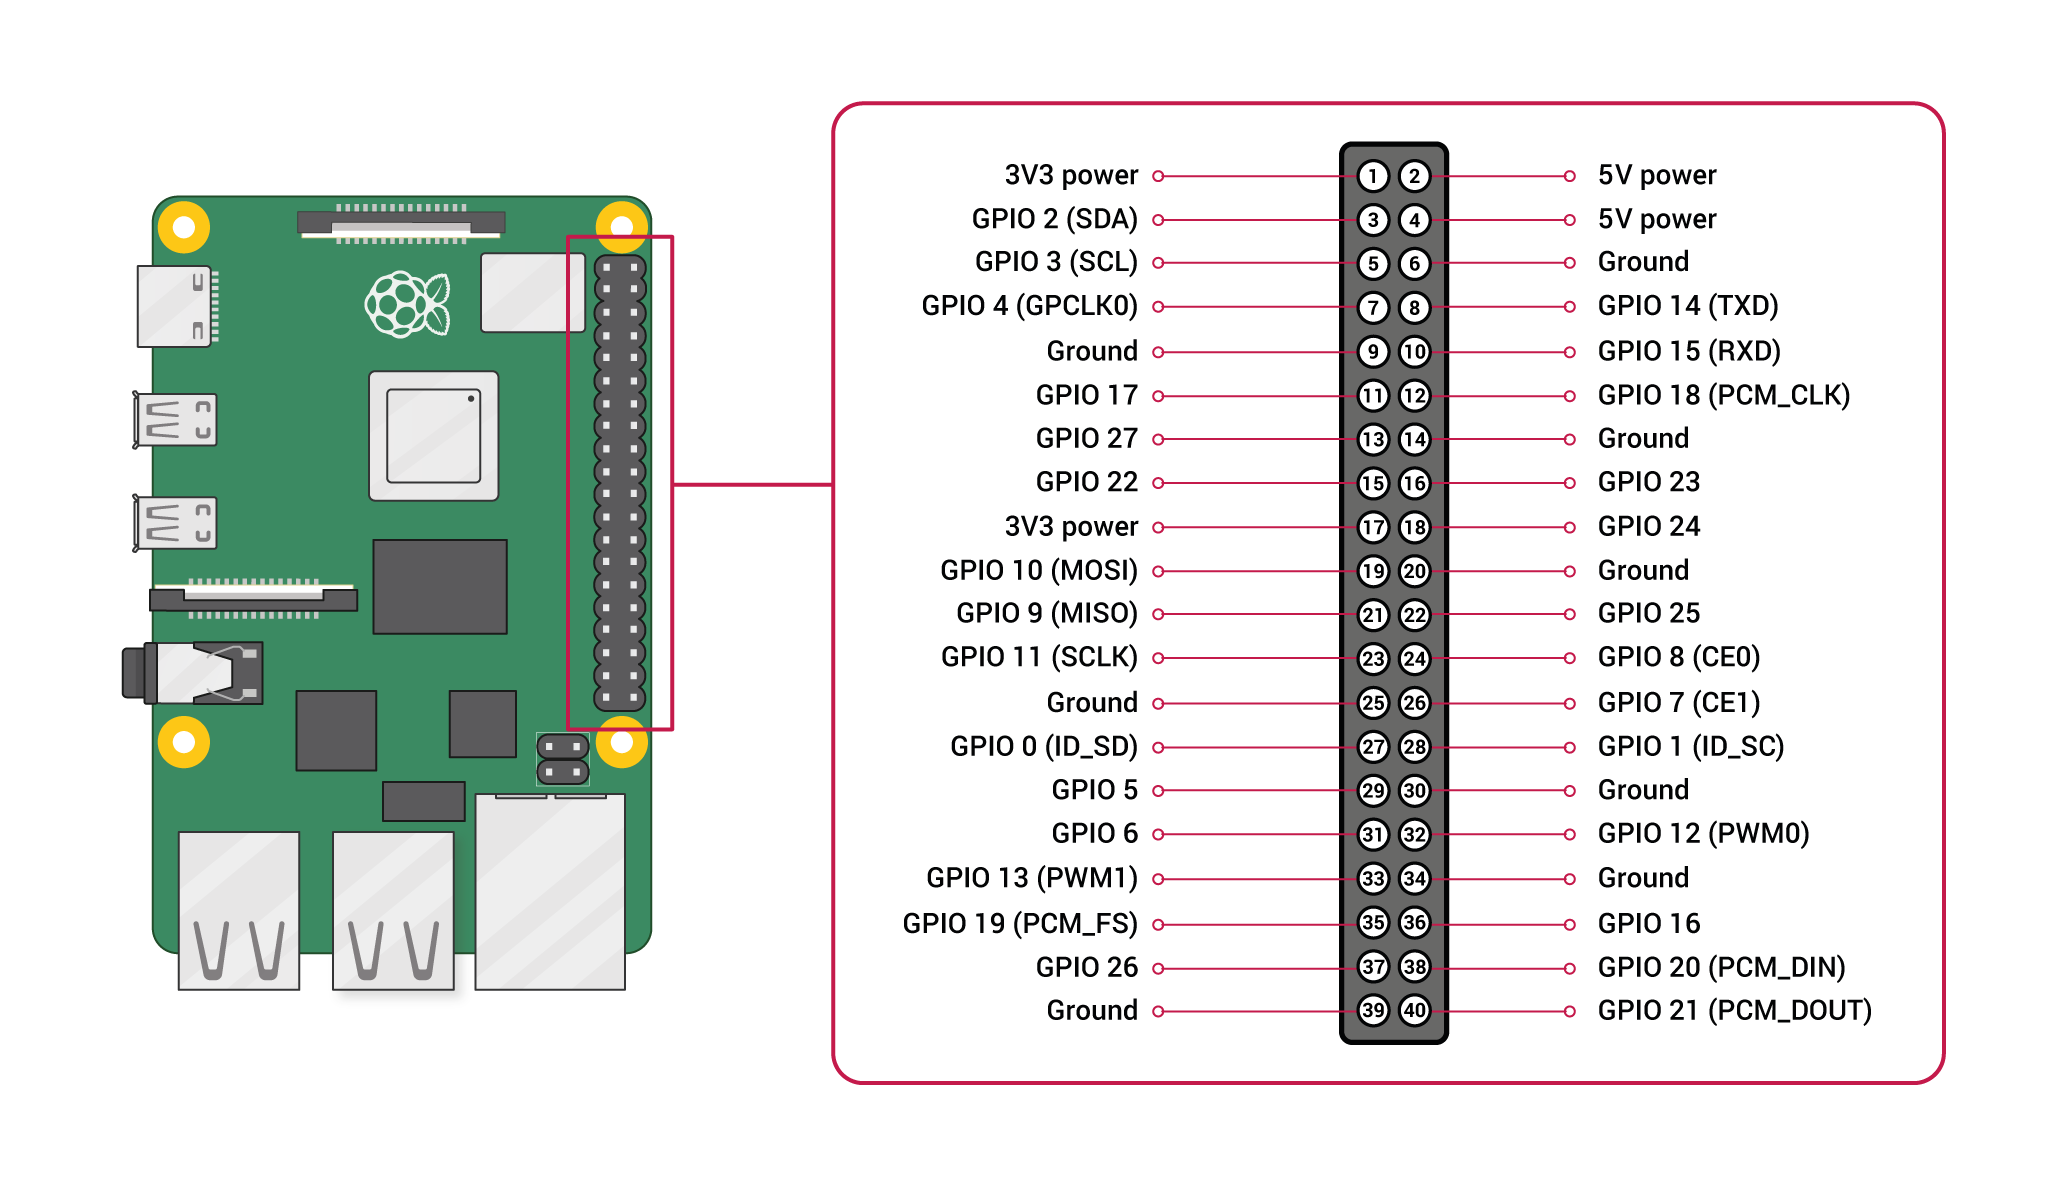
\includegraphics{obrazky-figures/gpio.png}
    }
  \caption{Rozložení pinů na Raspberry Pi \cite{rpi_doku}.}\label{pic:gpio_pinout}
\end{figure}

\section{Měření jednotky}
Cílem tohoto testu bylo ověřit, zda RPi vyčítá data o~správné vzorkovací rychlosti z~rozšiřující desky nebo souboru a nedochází ke ztrátě dat. Pokud jednotka čte data ze souboru, je vyveden hodinový signál o~nastavené frekvenci na jeden z~GPIO pinů a tento pin je fyzicky propojen s~pinem nastaveným jako \textit{data ready}. Výstupní frekvence výstupního pinu byla změřena pomocí osciloskopu. Na obrázku \ref{pic:gpio_pinout} je možné vidět rozložení pinů na RPi. Sonda byla připojena k~vývodu hodinového signálu na pinu číslo 7 (GPCLK0). Frekvence výstupního signálu byla nastavena na 128 kHz a souhlasila s~hodnotou odečtenou na osciloskopu. Rychlost čtení z~rozhraní SPI byla také ověřována pomocí osciloskopu. K~RPi s~připojenou rozšiřující deskou byly připojeny dvě sondy. Prví sonda byla připojena k~pinu číslo 15 (GPIO 22), na který je přiváděn signál \textit{data ready}. Druhá sonda byla připojena na pin číslo 21 (GPIO 9), který funguje jako MISO (Master In Slave Out -- příchozí data z~SPI od rozšiřující desky). Komunikace byla zaznamenána nejdříve při vzorkovací frekvenci 64 kHz a posléze i při frekvenci 128 kHz. Část komunikace mezi deskou a RPi z~prvního testu je možné vidět na obrázku \ref{pic:osciloscop}.

\begin{figure}[h]
  \centering
  \scalebox{0.22}{
        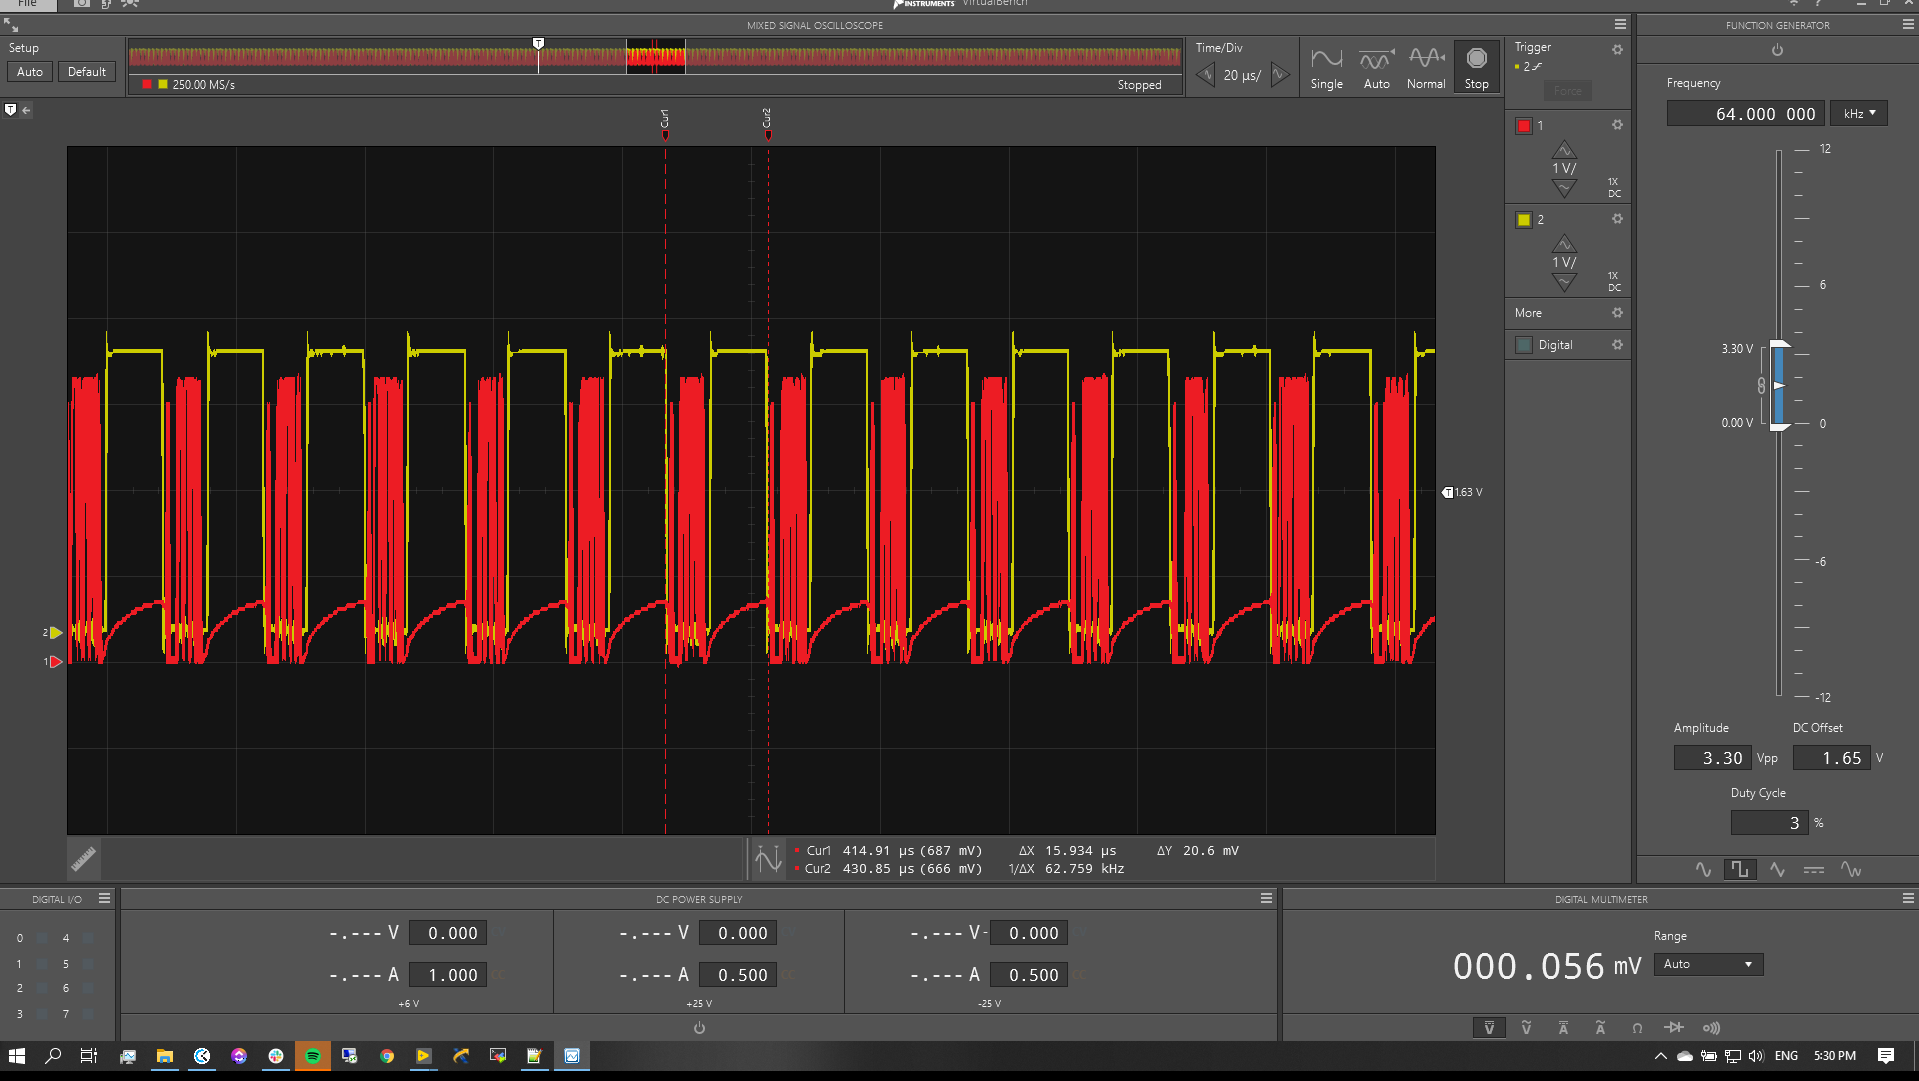
\includegraphics{obrazky-figures/osciloskop64kHz.png}
    }
  \caption{Komunikace přes SPI při 64 kHz mezi RPi a rozšiřující deskou.}\label{pic:osciloscop}
\end{figure}

Na obrázku je možné vidět žlutě značený signál \textit{data ready}. Signál má skutečně frekvenci 64 kHz, nastavení AD převodníku tudíž proběhlo správně. Červeně značený signál značí čtení dat z~převodníku. Data jsou čtena při sestupné hraně signálu \textit{data ready}. V~měření nebylo jediné vynechání čtení. Z~obrázku je patrné, že RPi strávilo čtením dat méně než polovinu doby před příchodem další sestupné hrany. Stejným způsobem bylo změřeno i čtení dat o~vzorkovací frekvenci 128 kHz. Stejně jako při předchozím testu nedocházelo k~vynechání dat, zařízení využívalo zhruba 90 \% času mezi jednotlivými sestupnými hranami pro čtení. Vyšší vzorkovací frekvenci by testovaná implementace nestíhala číst.

\section{Detekce překročení limitu s~historickými daty}
Cílem testu bylo ověřit sledování příchozích dat do databáze a upozornění na překročení limitu u~senzoru. K~testu byla využita historická agregovaná data partnerské firmy obsahující poruchu stroje. Data byla obdržena ve formátu csv. Pro účely testu byl vytvořen program \textit{CSVImport}, umístěný na přiloženém médiu ve složce \textit{Testing/}. Vstupními argumenty jsou \textit{-f <soubor>} s~názvem souboru, který má být importován, \textit{-a <ipv4>} adresa serveru a \textit{-p <port>} s~portem cílového serveru. Program postupně čte hodnoty ze souboru a vytváří UDP zprávy, které odesílá UDP serveru. Pro tento test nemohlo být využito čtení ze souboru na jednotce, protože byly poskytnuty již agregované hodnoty a implementace čtení ze souboru na jednotce vyžaduje nezpracovaná data o~nastavené vzorkovací frekvenci. Csv soubor \textit{data.csv}, použitý k~tomuto testu, je umístěn na přiloženém médiu v~kořenovém adresáři. Každý řádek souboru obsahuje unixovou časovou značku v~milisekundách a naměřenou hodnotu.

K~detekci překonání nastaveného limitu hodnoty bylo využito nástroje Kapacitor, dostupného s~databází InfluxDB. Při instalaci nástroje bylo postupováno podle dokumentace\footnote{https://docs.influxdata.com/kapacitor/v1.5/introduction/installation/}. Po spuštění nástroje je možné ho ovládat přes webové rozhraní Chronograf. Limit poruchy byl u~partnerské firmy nastaven na hodnotu 0.45, pro účely testu byla nastavena stejná hodnota. Jako způsob upozornění o~překročení limitu bylo zvoleno odeslání emailu. Data byla odesílána po jedné vteřině a okamžitě po překročení nastaveného limitu byl odeslán email s~přednastavenou zprávou na zvolenou emailovou adresu. Stránku pro správu upozornění i s~překročenou hodnotou je možné vidět na obrázku \ref{pic:alert}. 

Test prokázal schopnost implementovaného systému upozornit uživatele při překročení nastaveného limitu jednotky. 

\begin{figure}[h]
  \centering
  \scalebox{0.22}{
        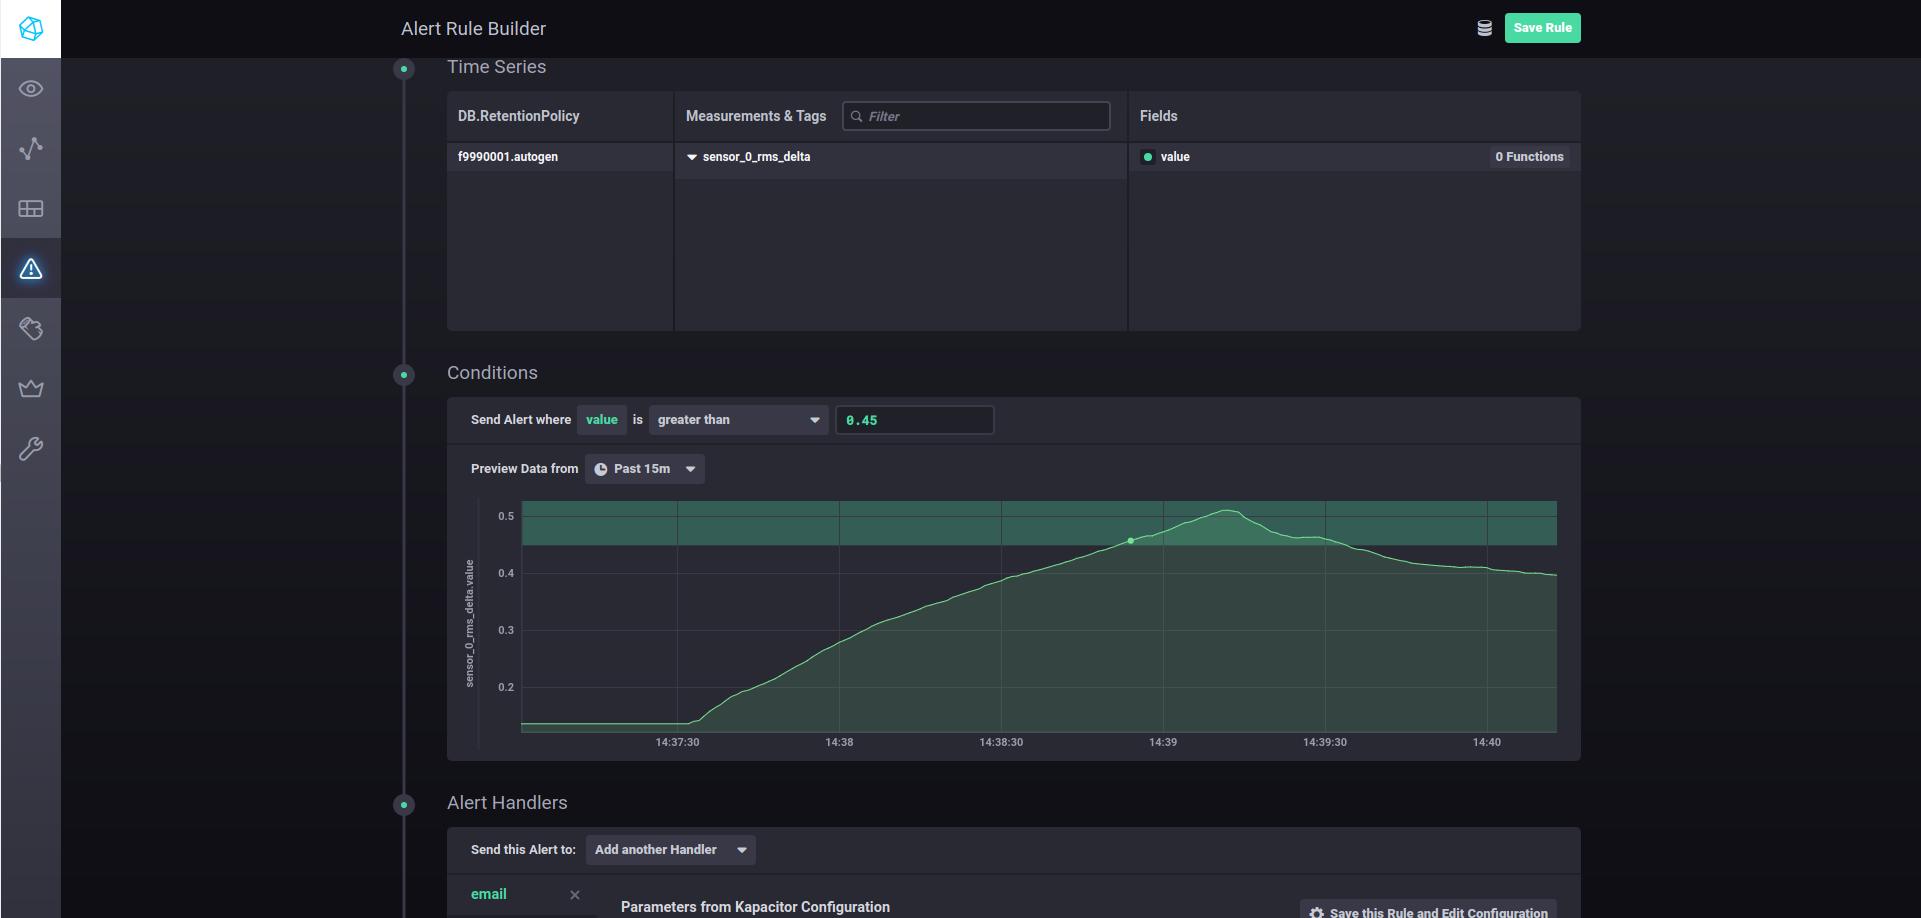
\includegraphics{obrazky-figures/alert.png}
    }
  \caption{Správa pravidla pro Kapacitor v~aplikaci Chronograf.}\label{pic:alert}
\end{figure}



\chapter{Závěr}
Cílem této práce bylo navrhnout a implementovat systém pro sběr a zpracování dat ze senzorů dostupných v~průmyslových provozech. Výsledný systém obsahuje serverovou část, jednotku a komunikační protokoly pro zasílání dat. Serverový systém je navržen a implementován tak, aby mohl operovat pouze na jednom zařízení a zvládal přitom zpracovávat data nejméně padesáti jednotek. Zároveň, pokud je potřeba počet jednotek navýšit, je možné systém rozložit na více zařízení a jednotlivé komponenty škálovat. Serverové aplikace byly vytvořeny v~jazyce C++ a jsou určeny pro operační systém Ubuntu server. Pro ukládání informací o~systému je využita relační databáze a jako úložiště měřených dat je použita časová databáze. Jednotka byla poskytnuta partnerskou firmou a skládá se z~počítače Raspberry Pi a rozšiřující desky s~konektory pro čtyři senzory vibrací. Rozšiřující deska vzorkuje data ze senzorů o~frekvenci 128000 Hz. Software jednotky, implementovaný v~této práci, je tedy schopný zpracovávat až půl milionu hodnot za vteřinu. Data jsou odesílána na serverovou část dvěma způsoby. První způsob využívá navržený komunikační protokol \ref{pic:udp_protocol} postavený na UDP. Zprávy obsahují filtrované, agregované hodnoty s~frekvencí až sto hodnot za vteřinu, sloužící pro odhalení poruchy. Druhý způsob využívá protokol \ref{pic:tcp_protocol} postavený na TCP. Zprávy potom obsahují bloky nezpracovaných dat a umožňují provádění pokročilých analýz na serveru. V obou případech mohou být zprávy podle nastavení jednotky zašifrované. K~zabezpečení UDP zpráv je využito metody XOR šifrování, k~zabezpečení TCP spojení je využito SSL. Software jednotky je implementován v~jazyce C++ a obsahuje i instalační skripty pro rychlou a bezzásahovou instalaci.


Základními požadavky na systém je jeho škálovatelnost, rychlost a modularita. Škálovatelnost serverové části je dosažena několika metodami popsanými v~\ref{sec:load_balancing}. Systém je implementován tak, aby veškeré komponenty bylo možné samostatně škálovat. Serverová část také není závislá na implementaci jednotky, data mohou přicházet i od jiného typu jednotek než té implementované v~této práci. Musí ovšem využívat navržené komunikační protokoly. Systém je také navržen na více typů senzorů. Na historických datech partnerské firmy byla ověřena schopnost systému upozornit uživatele při poruše stroje detekované překročením nastaveného limitu u~příchozích dat.

Přínos této práce je ve využití volně dostupných systémů, jako je ekosystém TICK, pro zpracování velkých dat s~levnými jednodeskovými zařízeními pro sběr dat, jako je například Raspberry Pi. Propojením volně dostupných knihoven a programů je možné vytvořit škálovatelný systém pro monitorování průmyslových strojů, na kterém je možné stavět další pokročilejší funkcionalitu. Takové řešení je v porovnání s dostupnými komerčními produkty, které jsou většinou šity na míru, řádově levnější a univerzálnější. To potvrzuje i snaha partnerské firmy o pokračování vývoje systému navrženého a implementovaného v této práci a zájmu zákazníků o aplikaci podobných systémů v praxi (ZKL, Škoda Auto a podobně).



  \fi
  
  % Kompilace po částech (viz výše, nutno odkomentovat)
  % Compilation piecewise (see above, it is necessary to uncomment it)
  %\subfile{projekt-01-uvod-introduction}
  % ...
  %\subfile{chapters/projekt-05-conclusion}


  % Pouzita literatura / Bibliography
  % ----------------------------------------------
\ifslovak
  \makeatletter
  \def\@openbib@code{\addcontentsline{toc}{chapter}{Literatúra}}
  \makeatother
  \bibliographystyle{bib-styles/Pysny/skplain}
\else
  \ifczech
    \makeatletter
    \def\@openbib@code{\addcontentsline{toc}{chapter}{Literatura}}
    \makeatother
    \bibliographystyle{bib-styles/Pysny/czplain}
  \else 
    \makeatletter
    \def\@openbib@code{\addcontentsline{toc}{chapter}{Bibliography}}
    \makeatother
    \bibliographystyle{bib-styles/Pysny/enplain}
  %  \bibliographystyle{alpha}
  \fi
\fi
  \begin{flushleft}
  \bibliography{projekt-20-literatura-bibliography}
  \end{flushleft}

  % vynechani stranky v oboustrannem rezimu
  % Skip the page in the two-sided mode
  \iftwoside
    \cleardoublepage
  \fi

  % Prilohy / Appendices
  % ---------------------------------------------
  \appendix
\ifczech
  \renewcommand{\appendixpagename}{Přílohy}
  \renewcommand{\appendixtocname}{Přílohy}
  \renewcommand{\appendixname}{Příloha}
\fi
\ifslovak
  \renewcommand{\appendixpagename}{Prílohy}
  \renewcommand{\appendixtocname}{Prílohy}
  \renewcommand{\appendixname}{Príloha}
\fi
%  \appendixpage

% vynechani stranky v oboustrannem rezimu
% Skip the page in the two-sided mode
%\iftwoside
%  \cleardoublepage
%\fi
  
\ifslovak
%  \section*{Zoznam príloh}
%  \addcontentsline{toc}{section}{Zoznam príloh}
\else
  \ifczech
%    \section*{Seznam příloh}
%    \addcontentsline{toc}{section}{Seznam příloh}
  \else
%    \section*{List of Appendices}
%    \addcontentsline{toc}{section}{List of Appendices}
  \fi
\fi
  \startcontents[chapters]
  \setlength{\parskip}{0pt} 
  % seznam příloh / list of appendices
  % \printcontents[chapters]{l}{0}{\setcounter{tocdepth}{2}}
  
  \ifODSAZ
    \setlength{\parskip}{0.5\bigskipamount}
  \else
    \setlength{\parskip}{0pt}
  \fi
  
  % vynechani stranky v oboustrannem rezimu
  \iftwoside
    \cleardoublepage
  \fi
  
  % Přílohy / Appendices
  \ifenglish
    \input{projekt-30-prilohy-appendices-en}
  \else
    \chapter{Příkazy a soubory}\label{att:server_install}
Tato sekce obsahuje potřebné příkazy a ukázky souborů.


\section{SSH}\label{att:ssh}
\begin{lstlisting}[language=bash,breaklines]
    $ sudo apt install openssh-server #install ssh
    $ sudo sed -i 's/#Port 22/Port 60022/g' /etc/ssh/sshd_config #change ssh port
    $ sudo sed -i 's/#PermitRootLogin prohibit-password/PermitRootLogin no/g' /etc/ssh/sshd_config #disable root login
    $ sudo ufw allow 60022/tcp #allow new ssh port
    $ sudo systemctl restart ssh #restart ssh service
\end{lstlisting}

\section{Potřebné knihovny pro server}\label{att:server_libs}
\begin{lstlisting}[language=bash,breaklines]
    $ sudo apt install libzip-dev
    $ sudo apt install cmake
    $ sudo apt install git
    $ sudo apt install libmysqlcppconn-dev
    $ sudo apt install pkg-config libcurlpp-dev libcurl4-openssl-dev
    $ sudo apt install libboost-all-dev
    $ sudo apt install libssl-dev
\end{lstlisting}

\section{Přeložení projektů na serveru}\label{att:compile}
\begin{lstlisting}[language=bash,breaklines]
    $ mkdir build
    $ cd build
    $ cmake ..
    $ make
\end{lstlisting}


%\section{InfluxDB}\label{att:influx}
%\begin{lstlisting}[language=bash,breaklines]
%    $ wget -qO- https://repos.influxdata.com/influxdb.key | sudo apt-key add - source /etc/lsb-release
%    $ echo "deb https://repos.influxdata.com/${DISTRIB_ID,,} ${DISTRIB_CODENAME} stable" | sudo tee %/etc/apt/sources.list.d/influxdb.list
%\end{lstlisting}
  \fi
  
  % Kompilace po částech (viz výše, nutno odkomentovat)
  % Compilation piecewise (see above, it is necessary to uncomment it)
  %\subfile{projekt-30-prilohy-appendices}
  
\end{document}
